%!TEX root = ../thesis.tex
%*******************************************************************************
%****************************** Fourth Chapter **********************************
%*******************************************************************************
\chapter{ElecSim model}
\label{chapter:elecsim}

% **************************** Define Graphics Path **************************
\ifpdf
    \graphicspath{{Chapter3/Figs/Raster/}{Chapter3/Figs/PDF/}{Chapter3/Figs/}}
\else
    \graphicspath{{Chapter3/Figs/Vector/}{Chapter3/Figs/}}
\fi

\section*{Prologue}

In this Chapter we motivate and introduce the agent-based model, ElecSim. 

The majority of the work presented in this paper has been presented in \cite{Kell} and \cite{Kell2020}.

%%%%%%%%%%%%%%%%%%%%%%%%%%%%%%%%
%%%%%%%%%%%%%%%% Paper 1
%%%%%%%%%%%%%%%%%%%%%%%%%%%%%%%%

The contribution of this Chapter is a new open-source framework with example scenarios of varying carbon taxes. We provide curated data, and improve realism via Monte-Carlo sampling. Section \ref{Literature Review} is a literature review. Section \ref{Model} details the model and assumptions made, and Section \ref{Validation and Performance} provides performance metrics and validation. Section \ref{Scenario Testing} details our results. We conclude the work in Section \ref{Conclusion}.


%%%%%%%%%%%%%%%%%%%%%%%%%%%%%%%%
%%%%%%%%%%%%%%%% Paper 2
%%%%%%%%%%%%%%%%%%%%%%%%%%%%%%%%




	% Background
	
	Electricity market modelling is often used by governments, industry and agencies to explore the development of scenarios over differing timeframes. For example, what would the reduction in cost of renewable energy mean for investments in gas power plants or what would be an optimum strategy for carbon tax or subsidies? %Or, how might an increase in demand from electric vehicles impact on investment and electricity prices? 
	
	Optimization based solutions are the dominant approach for analysing energy policy. However, these types of models have certain limitations such as the need to be interpreted in a normative manner, and the assumption that the electricity market remains in equilibrium throughout. Through this work, we show that agent-based models are a viable technique to simulate decentralised electricity markets. The aim of this paper is to validate an agent-based modelling framework to increase confidence in its ability to be used in policy and decision making. 
	
	% Methodology
	
	
	Our framework is able to model heterogenous agents with imperfect information. The model uses a rules-based approach to approximate the underlying dynamics of a real life, decentralised electricity market. We use the UK as a case-study, however our framework is generalisable to other countries. We increase the temporal granularity of the model by selecting representative days of electricity demand and weather using a $k$-means clustering approach. 
	
	
	% Results  
	
	
	We show that our modified framework, ElecSim, is able to adequately model the transition from coal to gas observed in the UK between 2013 and 2018. We are also able to simulate a future scenario to 2035 which is similar to the UK Government, Department for Business and Industrial Strategy (BEIS) predictions, showing a more realistic increase in nuclear power over this time period. This is due to the fact that with current, large nuclear technology, electricity is generated almost instantaneously and has a low relative short-run marginal cost \cite{Department2016}. This low short-run marginal cost means that new nuclear will be dispatched on the electricity market once it has been turned on, and thus will not increase gradually.
	
	
	
	



In Section \ref{lit-review} we introduce a review of techniques used for validating electricity market models as well as fundamental challenges of electricity model validation. Section \ref{ssec:prob_formulation} explores our approach to validate our model. In Section \ref{sec:details} we discuss the modifications made to our model to improve the results of validation. In Section \ref{sec:results} we present our results, and we conclude in Section \ref{sec:conclusion}.


\section{Introduction and Motivation}


\subsection{Transition to a low-carbon energy supply}

Global carbon emissions from fossil fuels have significantly increased since 1900 \cite{boden2017global}.    Fossil-fuel based electricity generation sources such as coal and natural gas currently provide 65\% of global electricity. Low-carbon sources such as solar, wind, hydro and nuclear provide 35\% \cite{BP2018}. To halt this increase in \ce{CO2} emissions, a transition of the energy system towards a renewable energy system is required. 

% To achieve a low carbon energy infrastructure, and limit the effects of global warming, a transition in the electricity mix is required. Moving from a centralised and homogenous fossil fuel-based system to a distributed system based on renewable energy and batteries. % Batteries are required due to the fact that most renewable sources are effected by conditions outside the control of the owners (e.g. time of day, wind speed and cloud cover). This leads to a need for electricity to be stored at times when renewable production exceeds renewable energy supply, and for the batteries to be discharged at times of high electrical demand and low renewable energy supply. 




Such a transition needs to be performed in a safe and non-disruptive manner -- it may be possible to close down all fossil fuel plants in the next year, though if this leads to electricity shortages and power cuts then this is likely to cause significant problems both for companies and homes. Therefore a stepped approach which allows seamless transfer is desirable. This may seem a simple process to achieve -- slowly phase out existing fossil fuel generators and replace these by renewable sources -- however, there are many risks and uncertainties in this process. Existing power plants have an expected lifetime and their owners wish to maximise this and the profits which can be made from them, renewable sources are still developing -- meaning that their efficiency and reliability will change in years to come.

Due to the long construction times, operating periods and high costs of power plants, investment decisions can have long term impacts on future electricity supply \cite{Chappin2017}. Governments and society, therefore, have a role in ensuring that the negative externalities of emissions are priced into electricity generation. This is most likely to be achieved via a carbon tax and regulation to influence electricity market players such as generation companies (GenCos).


Decisions made in an electricity markets may have unintended consequences due to their complexity. A method to test hypothesise before they are implemented would therefore be useful.

To aid in such a transition, energy modelling can be used by governments, industry and agencies to explore possible scenarios under different variants of government policy, future electricity generation costs and energy demand. These energy modelling tools aim to mimic the behaviour of energy systems through different sets of equations and data sets to determine the energy interactions between different actors and the economy \cite{Machado2019}.





\subsection{ElecSim: Modelling and simulation}




Live experimentation of physical processes is often not practical. The costs of real life experimentation can be prohibitively high, and can require significant time in order to fully ascertain the long-term trends. There is also a risk that changes can have detrimental impacts and lead to risk-averse behaviour. These factors are true for electricity markets, where decisions can have long term impacts. Simulation, however, can be used for rapidly prototyping ideas. The simulation is parametrised by real world data and phenomena. Through simulation, the user is able to assess the likelihoods of outcomes under certain scenarios and parameters \cite{Law:603360}.





Simulation is often used to increase understanding as well as to reduce risk and reduce uncertainty. Simulation allows practitioners to realise a physical system in a virtual model. In this context, a model is defined as an approximation of a system through the use of mathematical formulas and algorithms. Through simulation, it is possible to test a system where real life experimentation would not be practical due to reasons such as prohibitively high costs, time constraints or risk of detrimental impacts. This has the dual benefit of minimising the risk of real decisions in the physical system, as well as allowing practitioners to test less risk-averse strategies.

\acrfull{abm}s are a class of computational simulation models composed of autonomous, interacting agents and model the dynamics of a system. Due to the numerous and diverse actors involved in electricity markets, \acrshort{abm}s have been utilised in this field to address phenomena such as market power \cite{Ringler2016a}. 

The work presented in this Chapter develops ElecSim, an open-source \acrshort{abm} that simulates GenCos in a wholesale electricity market. ElecSim models each GenCo as an independent agent and electricity demand. An electricity market facilitates trades between the two. 

GenCos make bids for each of their power plants. Their bids are based on the generator's short run marginal cost (SRMC) \cite{Perloff2012}, which excludes capital and fixed costs. The electricity market accepts bids in cost order, also known as merit-order dispatch. GenCos invest in power plants based on expected profitability.	

ElecSim is designed to provide quantitative advice to policy makers, allowing them to test policy outcomes under different scenarios. They are able to modify a scenario file to realise a scenario of their choice. It can also be used by energy market developers who can test new electricity sources or policy types, enabling the modelling of changing market conditions.

 This model can be used by the following players:
 
 \begin{itemize}
 \item {\bf Policy experts} to test policy outcomes under different scenarios and provide quantitative advice to policy makers. They can provide a simple script defining the policies they wish to use along with the parameters for these polices.
 \item {\bf Energy market developers} who can use the extensible framework to add such things as new energy sources, policy types, consumer profiles and storage types. Thus allowing ElecSim to adapt to a changing ecosystem.
 \end{itemize}
 



% \begin{figure}
% \centering
% 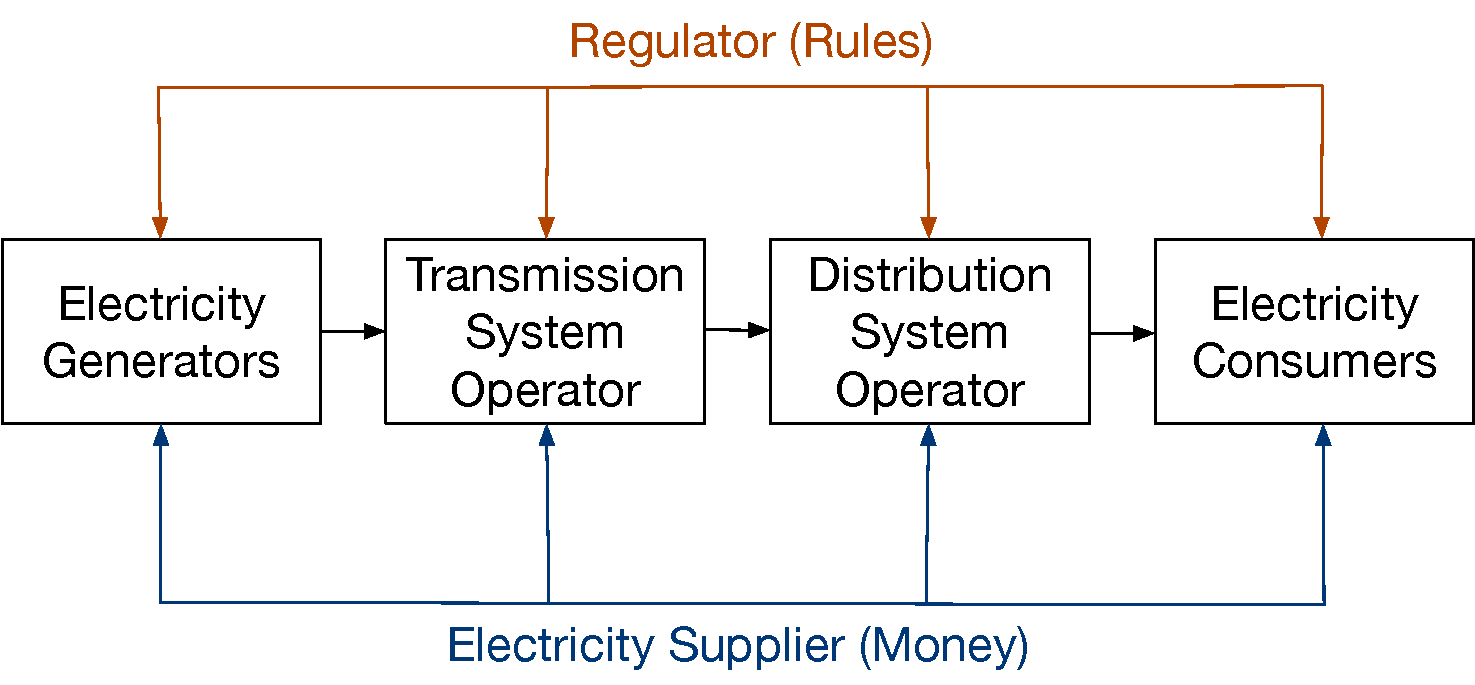
\includegraphics[width=0.9\linewidth]{figures/main_electricty_players}
% \caption{{\color{red}Schematic overview of the electricity system \cite{Erbach2016}.}}
% \label{fig:mainelectrictyplayers}
% \end{figure}

%%%%%%%%%%%%%%%%%%%%%%%%%%%%%%%%%%%%%%%%%%%%%%%%
%%%%%%%%%%%%%%%%%%%%%%%%      Paper 2    %%%%%%%%%%%%%%%%
%%%%%%%%%%%%%%%%%%%%%%%%%%%%%%%%%%%%%%%%%%%%%%%%

Optimization based solutions are the dominant approach for analysing energy policy \cite{Chappin2017}. However, the results of these models should be interpreted in a normative manner. For example, how investment and policy choices should be carried out, under certain assumptions and scenarios. The processes which emerge from an equilibrium model remain a black-box, making it difficult to fully understand the underlying dynamics of the model \cite{Chappin2017}. 



In addition to this, optimization models do not allow for  endogenous behaviour to emerge from typical market movements, such as investment cycles \cite{Chappin2017, Gross2007}. By modelling these naturally occurring behaviours, policy can be designed that is robust against movements away from the optimum/equilibrium. Thus, helping policy to become more effective in the real world. 

Agent-based models differ from optimization models by the fact that they are able to explore `\textit{what-if}' questions regarding how a sector could develop under different prospective policies, as opposed to determining optimal trajectories. \acrshort{abm}s are particularly pertinent in decentralised electricity markets, where a centralised actor does not dictate investments made within the electricity sector. \acrshort{abm}s have the ability to closely mimic the real world by, for example, modelling irrational agents, in this case Generation Companies (GenCos) with incomplete information in uncertain situations \cite{Ghorbani2014}. 


To further enhance the perfomance of ElecSim, we use representative days to model a year time period. Similarly to Nahmmacher \textit{et al.} we demonstrate how clustering of multiple relevant time series such as electricity demand, solar irradiance and wind speed can reduce computational time by selecting representative days ~\cite{Nahmmacher2016}. In this context, representative days are a subset of days that have been chosen due to their ability to approximate the weather and electricity demand in an entire year. Distinct to Nahmacher \textit{et al.} we use a $k$-means clustering approach \cite{forgy65} as opposed to a hierarchical clustering algorithm described by Ward \cite{doi:10.1080/01621459.1963.10500845}. We chose the $k$-means clustering approach due to previous success of this technique in clustering time series \cite{Kell2018a}. 



\subsection{Validation of long-term models}

There is a desire to validate the ability of energy-models to make long-term predictions. Validation increases confidence in the outputs of a model and leads to an increase in trust amongst the public and policy makers. Energy models, however, are frequently criticised for being insufficiently validated, with the performance of models rarely checked against historical outcomes \cite{Beckman2011}.

In answer to this, we postulate that \acrshort{abm}s can provide accurate information to decision makers in the context of electricity markets. We increase the temporal granularity of the work by Kell \textit{et al.} \cite{Kell} and use genetic algorithms to tune the model to observed data enabling us to perform validation. This enables us to understand the parameters required to observe certain phenomena, as well as use these fitted parameters to make inferences about the future. 


%- A short description of the solution


We use a genetic algorithm approach to find an optimal set of price curves predicted by generation companies (GenCos) that adequately model observed investment behaviour in the real-life electricity market in the United Kingdom. Similar techniques can be employed for other countries of various sizes \cite{Kell}. 

We measure the accuracy of projections for our improved \acrshort{abm} with those of the UK Government's Department for Business, Energy and Industrial Strategy (BEIS) for the UK electricity market between 2013 and 2018. In addition to this, we compare our projections from 2018 to 2035 to those made by BEIS in 2018 \cite{DBEIS2019}.




\subsection{Results}

Through this validation process, we are able to adequately model the transitional dynamics of the electricity mix in the United Kingdom between 2013 and 2018. During this time there was an ${\sim}88\%$ drop in coal use, ${\sim}44\%$ increase in Combined Cycle Gas Turbines (CCGT), ${\sim}111\% $ increase in wind energy and increase in solar from near zero to ${\sim}1250$MW. We are therefore able to test our model in a transition of sufficient magnitude.

%- What are the key take-home messages

We show in this Chapter, that agent-based models are able to mimic the behaviour of the UK electricity market under the same specific scenario conditions. Concretely, we show that under an observed carbon tax strategy, fuel price and electricity demand scenario, the model, ElecSim, closely matches the observed electricity mix between 2013 and 2018. We achieve this by determining an exogenous predicted price duration curve using a genetic algorithm to minimise error between observed and simulated electricity mix in 2018. The predicted price curve is an arrangement of all price levels in descending order of magnitude. The predicted price duration curve achieved is similar to that of the simulated price duration curve in 2018, increasing confidence in the underlying dynamics of our model. 

In addition, we compare our projections to those of the BEIS reference scenario from 2018 to 2035~\cite{DBEIS2019}. To achieve this, we use the same genetic algorithm optimisation technique as during our validation stage, optimising for predicted price duration curves. Our model demonstrates that we are able to closely match the projections of BEIS by finding a set of realistic price duration curves which are subject to investment cycles. Our model, however, exhibits a more realistic step change in nuclear output than that of BEIS. This is because, whilst BEIS projects a gradual increase in nuclear output, our model projects that nuclear output will grow instantaneously at a single point in time as a new nuclear power plant comes online. 

This allows us to verify the scenarios of other models, in this case BEIS' reference scenario, by ascertaining whether the optimal parameters required to achieve such scenarios are realistic. In addition to this, we are able to use these parameters to analyse `\textit{what-if}' questions with further accuracy.


\subsection{Contributions of this Chapter}
%- What are the key contributions

As part of this work we contribute a validated open-source agent-based model called ElecSim. Whilst we have used the United Kingdom as a use-case for this thesis, ElecSim is able to model decentralised markets of various sizes. 

To improve our results, we increased the temporal granularity of the model using a $k$-means clustering approach to select a subset of representative days for wind speed, solar irradiance and electricity demand. This subset of representative days enabled us to approximate an entire year and only required a fraction of the total time-steps that would be necessary to model each day of a year independently. This enabled us to decrease execution time. We show that we are able to provide an accurate framework, through this addition, to allow policy makers, decision makers and the public to explore the effects of policy on investment in electricity generators. 

We demonstrate that with a genetic algorithm approach we are able to optimise parameters to improve the accuracy of our model. Namely, we optimise the predicted electricity price, the uncertainty of this electricity price and nuclear subsidy. We validate our model using the observed electricity mix between 2013-2018.

A major contribution of this work is to demonstrate that it is possible for agent-based models to accurately model transitions in the UK electricity market. This was achieved by comparing our simulated electricity mix to the observed electricity mix between 2013 and 2018. In this time a transition from coal to natural gas was observed. We demonstrate that a high temporal granularity is required to accurately model fluctuations in wind and solar irradiance for intermittent renewable energy sources.


\clearpage
\section{Literature Review}


Whilst Chapter \ref{chapter:litreview} provided a review of the literature of models, this section covers the difficulties inherent in validating energy models and the approaches taken in the literature to validate these models..

\subsection{Limits of Validating Energy Models}

Beckman \textit{et al.} state that questions frequently arise as to how much faith one can put in energy model results. This is due to the fact that the performance of these models as a whole are rarely checked against historical outcomes~\cite{Beckman2011}.


Under the definition by Hodges \textit{et al.} \cite{Hodges} long-range energy forecasts are not validatable \cite{Craig2002}. Under this definition, validatable models must be observable, exhibit constancy of structure in time, exhibit constancy across variations in conditions not specified in the model and it must be possible to collect ample data \cite{Hodges}.


Whilst it is possible to collect data for energy models, the data covering important characteristics of energy markets are not always measured. Furthermore, the behaviour of the human population and innovation are neither constant nor entirely predictable. This leads to the fact that static models cannot keep pace with global long-term evolution. Assumptions made by the modeller may be challenged in the form of unpredictable events, such as the oil shock of 1973 \cite{Craig2002}.

This, however, does not mean that energy-modelling is not useful for providing advice in the present. A model may fail at predicting the long-term future because it has forecast an undesirable event, which led to a pre-emptive change in human behaviour. Thus avoiding the original scenario that was predicted. This could, therefore, be viewed as a success of the model.

Schurr \textit{et al.} argued against predicting too far ahead in energy modelling due to the uncertainties involved \cite{Schurr_1961}. However, they specify that long-term energy forecasting is useful to provide basic information on energy consumption and availability which is helpful in public debate and in guiding policy makers.


Ascher concurs with this view and states that the most significant factor in model accuracy is the time horizon of the forecast; the more distant the forecast target the less accurate the model. This can be due to unforeseen changes in society as a whole ~\cite{gillespie_1979}.

It is for these reasons that we focus on a shorter-term (5-year) horizon window when validating our model. This enables us to have an increased confidence that the dynamics of the model work without external shocks and can provide descriptive advice to stakeholders. However, it must be noted that the UK electricity market exhibited a fundamental transition from natural gas to coal electricity generation during this period, meaning that a simple data-driven modelling approach would not work.

In addition to this short-term cross-validation, we compare our long-term projections to those of BEIS from 2018 to 2035. It is possible that our projections and those of BEIS could be wrong, however, this allows us to thoroughly test a particular scenario with different modelling approaches, and allow for the possibility to identify potential flaws in the models.


\subsection{Validation Examples}

In this section we explore a variety of approaches used in the literature for energy model validation.

The model OSeMOSYS \cite{Howells2011} is validated against the similar model MARKAL\slash TIMES through the use of a case study named UTOPIA. UTOPIA is a simple test energy system bundled with ANSWER, a graphical user interface packaged with the MARKAL model generator \cite{Hunter2013, Noble2004}. Hunter \textit{et al.} use the same case study to validate their model Temoa \cite{Hunter2013}. In these cases, MARKAL\slash TIMES is seen as the "gold standard". In this paper, however, we argue that the ultimate gold standard should be real-world observations, as opposed to a hypothetical scenario.

The model PowerACE demonstrates that realistic prices are achieved by their modelling approach, however, they do not indicate success in modelling GenCo investment over a prolonged time period \cite{Ringler2012}.

Barazza \textit{et al}. validate their model, BRAIN-Energy, by comparing their results with a few years of historical data, however, they do not compare the simulated and observed electricity mix \cite{Barazza2020}.

Work by Koomey \textit{et al.} expresses the importance of conducting retrospective studies to help improve models \cite{Koomey2003}. In this case, a model can be rerun using historical data in order to determine how much of the error in the original forecast resulted from structural problems in the model itself, or how much of the error was due to incorrect specification of the fundamental drivers of the forecast \cite{Koomey2003}.

A retrospective study published in 2002 by Craig \textit{et al.} focused on the ability of forecasters to accurately predict electricity demand from the 1970s \cite{Craig2002}. They found that actual energy usage in 2000 was at the very lowest end of the forecasts, with only a single exception. They found that these forecasts underestimated unmodelled shocks such as the oil crises which led to an increase in energy efficiency.

Hoffman \textit{et al.} also developed a retrospective validation of a predecessor of the current MARKAL\slash TIMES model, named Reference Energy System \cite{Hoffman_1973}, and the Brookhaven Energy System Optimization Model \cite{ERDA_48}. These were studies applied in the 70s and 80s to develop projections to the year 2000. This study found that the models had the ability to be descriptive, but were not entirely accurate in terms of predictive ability. They found that emergent behaviours in response to policy had a strong impact on forecasting accuracy. The study concluded that forecasts must be expressed in highly conditioned terms \cite{Hoffman2011}. 




















\clearpage
\section{Architecture}
\label{elecsim:sec:architecture}

In this section we detail the architecture of how ElecSim has been designed.

ElecSim is made up of six parts: the agents, which are split up into demand and GenCos; power plants; a Power Exchange, which controls an electricity spot market; the time-steps ;and the data for parametrisation. A schematic of ElecSim is displayed in Figure \ref{fig:systemoverview}.

\begin{figure}
	\centering
	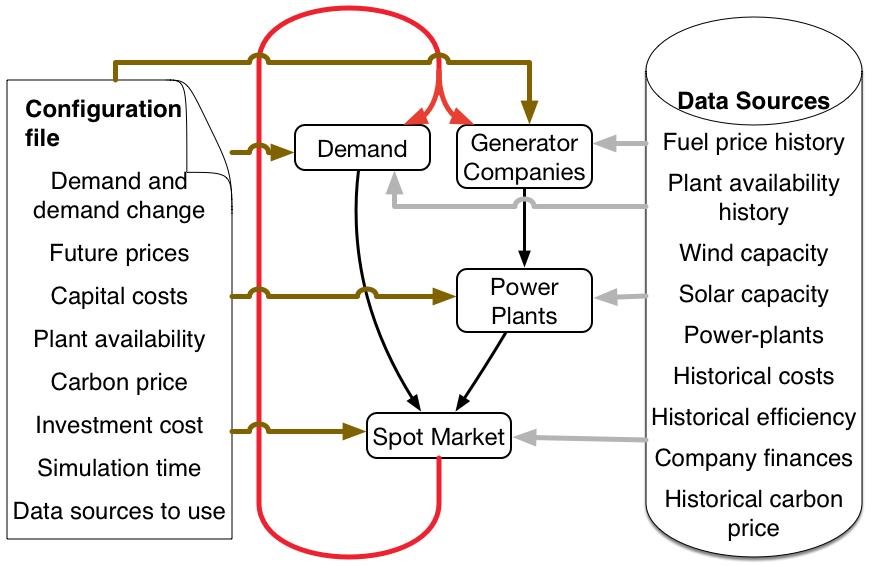
\includegraphics[width=0.85\linewidth]{Chapter4/figures/System_overview_large.png}
	\caption{High level overview.}
	\label{fig:systemoverview}
\end{figure}

\paragraph{Data parametrisation.} ElecSim contains a configuration file and a collection of data sources for parametrisation. These data sources contain information such as historical fuel prices, historical plant availability, wind and solar capacity.

The configuration file allows for rapid changes to test different hypothesis and scenarios, and points to the different data sources. The configuration file enables one to change the demand growth and shape, future fuel and carbon prices, capital costs, plant availability, investment costs and simulation time.

\paragraph{Demand Agent.} The demand agent is a simplified representation of aggregated demand in a country. The demand is represented as a load duration curve (LDC). An example load duration curve for a year is demonstrated in Figure \ref{fig:loaddurationcurve}. An LDC is an arrangement of all load levels in descending order of magnitude. where the lowest segment demand demonstrates baseload, and the highest segment represents peak demand. Each year, the demand agent changes each of the LDC segments proportionally.

 \begin{figure}
 	\centering
 	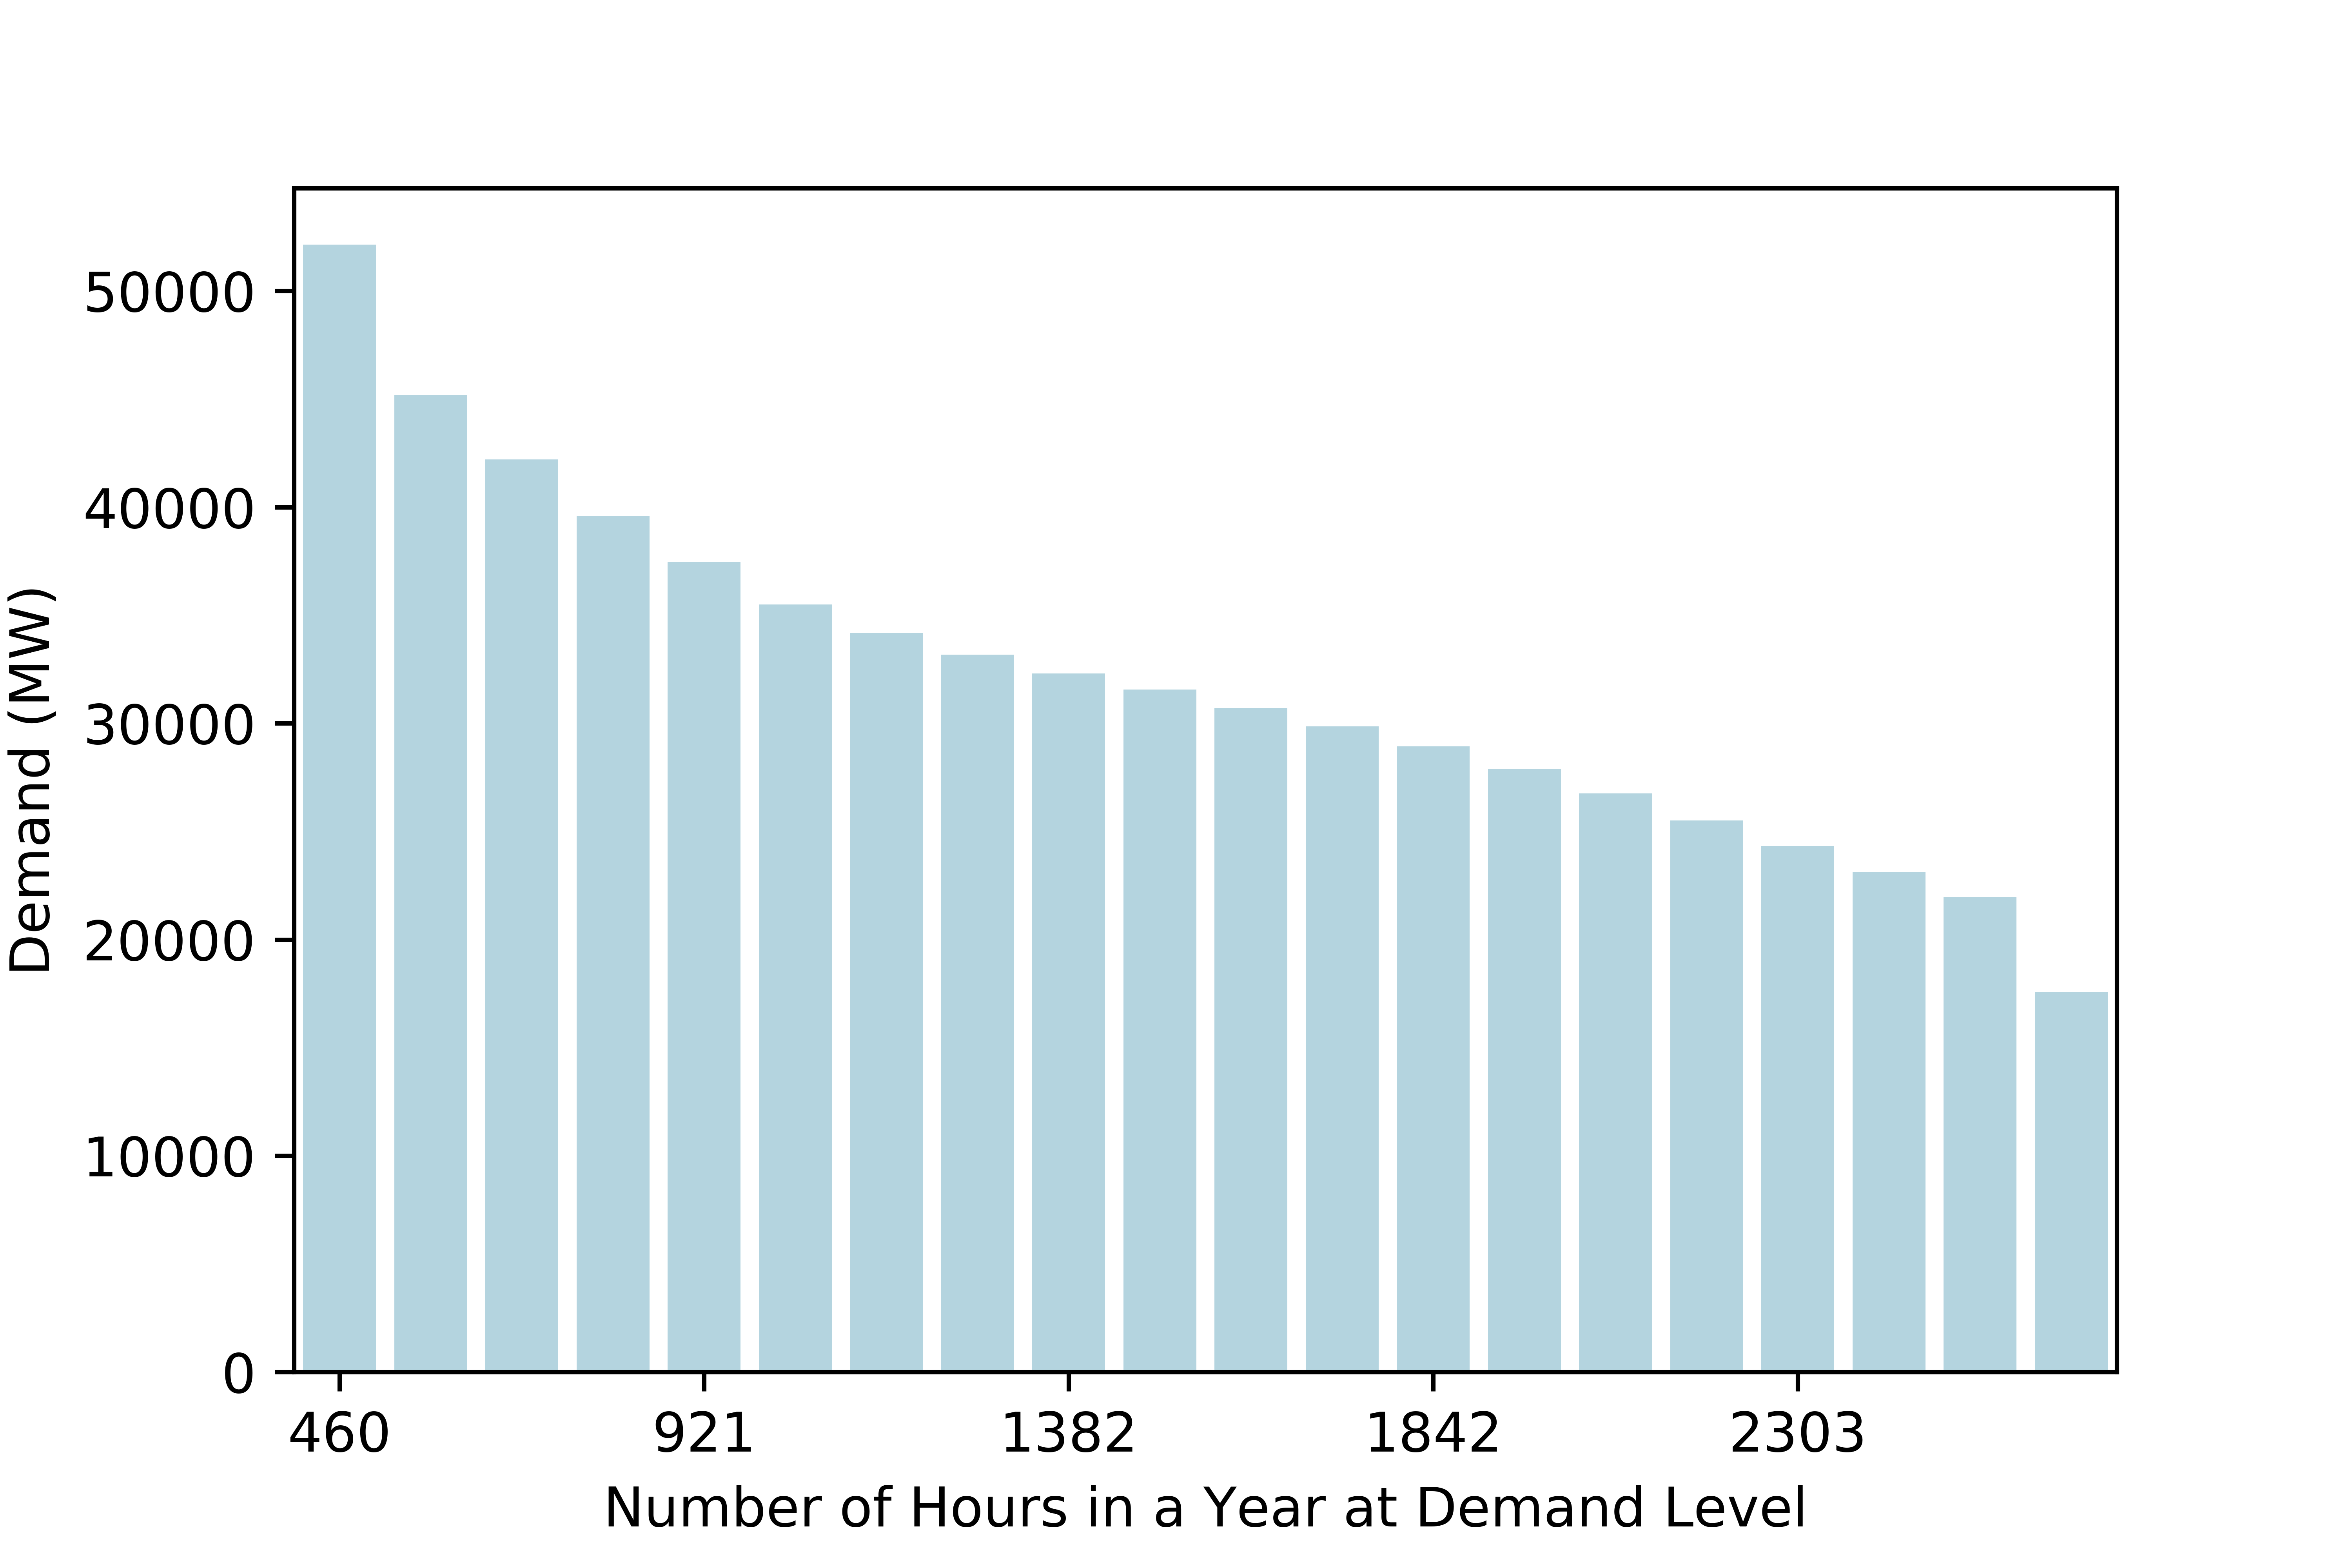
\includegraphics[width=0.95\linewidth]{Chapter4/figures/load_duration_curve}
 	\caption{Example load duration curve in a single year.}
  	\label{fig:loaddurationcurve}
 \end{figure}

%As per Chappin \textit{et al.} \cite{Chappin2017}, we modelled the LDC of electricity demand with twenty segments. Twenty segments enabled us to capture the variation in demand throughout the year to a high degree of accuracy, whilst reducing computational complexity. 


\paragraph{Generation Company Agents.} The GenCos have two main functions. Investing in power plants and making bids to sell their generation capacity. We will first focus on the buying and selling of electricity, and then cover the investment algorithm.

The power exchange runs every year, accepting the lowest bids until supply meets demand. Once this condition is met, the spot price or system marginal price (SMP) is paid to all generators regardless of their initial bid. Generators are motivated to bid their SRMC, to ensure that their generator is being utilised, and reduce the risk of overbidding.

\paragraph{Investment.} Investment in power plants is made based upon a net present value (NPV) calculation. NPV is a summation of the present value of a series of present and future cash flow. NPV provides a method for evaluating and comparing investments with cash flows spread over many years, making it suited for evaluating power plants which have a long lifetime.  \vphantom{\color{red}NPV is based upon the fact that current cash flow is worth more than future cash flow. This is due to the fact that money today can be invested and have a rate of return. This means that, for example \$50,000 today is worth more than \$50,000 in 10 years time. The value in which future cash flow is worth less than present cash flow is discounted by the discount rate.}

Equation \ref{architecture:eq:npv_eq} is the calculation of NPV, where $t$ is the year of the cash flow, $i$ is the discount rate, $N$ is total number of periods, or lifetime of power plant, and $R_t$ is the net cash flow at time $t$.
\begin{equation} \label{architecture:eq:npv_eq}
NPV(t, N) = \sum_{t=0}^{N}\frac{R_t}{(1+t)^t}
\end{equation}
A discount rate set by a GenCo's weighted average cost of capital (WACC) is often used \cite{KincheloeStephenC1990TWAC}. WACC is the rate that a company is expected to pay on average for its stock and debt. Therefore to achieve a positive NPV, an income larger than the WACC is required. However, a higher WACC is often selected to adjust for varying risk profiles, opportunity costs and rates of return. To account for these differences we sample from a Gaussian distribution, giving us sufficient variance whilst deviating from the expected price.

To calculate the NPV, future market conditions must be considered. For this, each GenCo forecasts $N$ years into the future, which we assume is representative of the lifetime of the plant. As in the real world, GenCos have imperfect information, and therefore must forecast expected demand, fuel prices, carbon price and electricity sale price. This is achieved by fitting functions to historical data. Each GenCo is different in that they will use differing historical time periods of data for forecasting.

Fuel and carbon price are forecast using linear regression. Demand, however, is forecast using an exponential function, which considers compounded growth. Linear regression is used if an exponential function is found to be sub-optimal.

The forecasted electricity price $N$ years ahead is difficult to ascertain accurately. We therefore use two methods for forecasting these. The first is to simulate a market $N$ years ahead. The second is to optimise for the predicted PDC using a genetic algorithm. We describe this optimisation in Section \ref{architecture:sec:validation}.

For the simulated market, the forecasted data is used to simulate a market $N$ years into the future using the electricity market algorithm. We simulate a market based on the expected bids -- based on SRMC -- that every operating power plant will make. This includes the removal of plants that will be past their operating period, and the introduction of plants that are in construction or pre-development stages. 

There may be scenarios where demand is forecast to grow significantly, and limited investments have yet been made to meet that demand. The expected price, would be that of lost load. Lost load is defined as the price customers would be willing to pay to avoid disruption in their electricity supply. To avoid GenCos from estimating large profits, and under the assumption that further power plant investments will be made, the lost load price is replaced with a predicted electricity price using linear regression based on prices at lower points of the demand curve. If zero segments of demand are met, then the  lost load price is used to encourage investment. 

Once this data has been forecasted, the NPV can be calculated. GenCos must typically provide a certain percentage of upfront capital, with the rest coming from investors in the form of stock and shares or debt (WACC). The percentage of upfront capital can be customised by the user in the configuration file. The GenCos then invest in the power plants with the highest NPV. 


\paragraph{Time-steps} For the time-steps, two approaches were taken. For the first approach, as per Chappin \textit{et al.} \cite{Chappin2017}, we modelled the LDC of electricity demand with twenty segments. Twenty segments enabled us to capture the variation in demand throughout the year to a high degree of accuracy, whilst reducing computational complexity. However, as we show later in Section \ref{elecsim:sec:scenarios}, this led to an overestimation of the supply of \acrshort{ires}. 

For the second approach, we used representative days to model a year. Representative days in this context are a subset of days which have characteristics, that when scaled proportionally can accurately model an entire year. To select these representative days we used a $k$-means approach. We describe this in full detail in Section \ref{elecsim:sec:representative}



\paragraph{Power Plant Parameters.}\label{elecsim:ssssec:powerplantparameters} Costs form an important element of markets and investment, and publicly available data for power plant costs for individual countries can be scarce. Thus, extrapolation and interpolation is required to estimate costs for power plants of differing sizes, types and years of construction.

Users are able to initialise costs relevant to their particular country by providing detailed cost parameters. They can also provide an average cost per MWh produced over the lifetime of a plant, known as levelised cost of electricity (LCOE).

The parameters used to initialise the power plants are detailed in this section. Periods have units of years and costs in \textsterling/MW unless otherwise stated: Efficiency ($\eta$) is defined as the percentage of energy from fuel that is converted into electrical energy (\%). Operating period ($OP$) is the total period in which a power plant is in operation. Pre-development period ($P_D$) and pre-development costs ($P_C$) include the time and costs for pre-licensing, technical and design, as well as costs incurred due to regulatory, licensing and public enquiry. The construction period ($C_D$) and construction costs ($C_C$) are incurred during the development of the plant, excluding network connections. The infrastructure costs ($I_C$) are the costs incurred by the developer in connecting the plant to the electricity or gas grid (\textsterling). Fixed operation \& maintenance costs ($F_C$) are costs incurred in operating the plant that do not vary based on output. Variable operation \& maintenance ($V_C$) costs are incurred in operating the plant that depend on generator output \cite{Ltd2016}.



%\begin{table}[h]
%	\centering
%	\csvautobooktabular{tables/notation_formated.csv}
%	\caption{Parameter notation. (Whilst the unit of currency displayed is \textsterling, this can be modified to other currencies eg. \$, \texteuro)}
%	\label{table:parameter_notation}
%\end{table}
%\addtolength{\textfloatsep}{-0.2in}

Precise data is not available for every plant size. Linear interpolation is used to estimate individual prices between known points. When the plant to be estimated falls outside of the range of known data points, the closest power plant is used. We experimented with extrapolation but this would often lead to unrealistic costs. %{\color{red}For example, the parameters of a 1,500MW combined cycle gas plant (CCGT) are estimated to be the same as a 1,200MW CCGT plant if the 1,200MW plant was the largest available data point. }

If specific parameters are not known, the LCOE can be used for parameter estimation, through the use of linear optimisation. Constraints can be set by the user, enabling, for example, varying operation and maintenance costs per country as a fraction of LCOE.

To fully parametrise power plants, availability and capacity factors are required. Availability is the percentage of time that a power plant can produce electricity. This can be reduced by forced or planned outages. We integrate historical data to model improvements in reliability over time.

The capacity factor is the actual electrical energy produced over a given time period divided by the maximum possible electrical energy it could have produced. The capacity factor can be impacted by regulatory constraints, market forces and resource availability. For example, higher capacity factors are common for photovoltaics in the summer, and lower in winter. 

To model the intermittency of wind and solar power we allow them to contribute only a certain percentage of their total capacity (nameplate capacity) for each load segment. This percentage is based upon empirical wind and solar capacity factors. In this calculation we consider the correlation between demand and renewable resources. 

When initialised, $V_C$ is selected from a uniform distribution, with the ability for the user to set maximum percentage increase or decrease. A uniform distribution was chosen to capture the large deviations that can occur in $V_C$, especially over a long time period. \vphantom{By doing this, the variance in costs between individual power plants for processes such as preventative and corrective maintenance, labour costs and skill, health and safety and chance are different per plant instant.}

Fuel price is controlled by the user, however, there is inherent volatility in fuel price. To take into account this variability, an ARIMA \cite{ARIMA} model was fit to historical gas and coal price data. The standard deviation of the residuals was used to model the variance in price that a GenCo will buy fuel in a given year. This considers differences in chance and hedging strategies.


%\vphantom{With historical power plants which have been refurbished, we sample their initialisation randomly between 15 years prior to the initialisation year and the initialisation year. This is done because there is rarely a comprehensive data set on when plants are refurbished. 15 years was chosen due to the fact that plants often have an operating period of 25 years, and therefore 15 years allowed for sufficient variance in results, whilst keeping plants in operation.}

Figure \ref{fig:lowlevelsystem} demonstrates the simulation and how it co-ordinates runs. The world contains data and brings together GenCos, the Power Exchange and demand. The investment decisions are based on future demand and costs, which in turn influence bids made.

\begin{landscape}
	\begin{figure*}
		\centering
		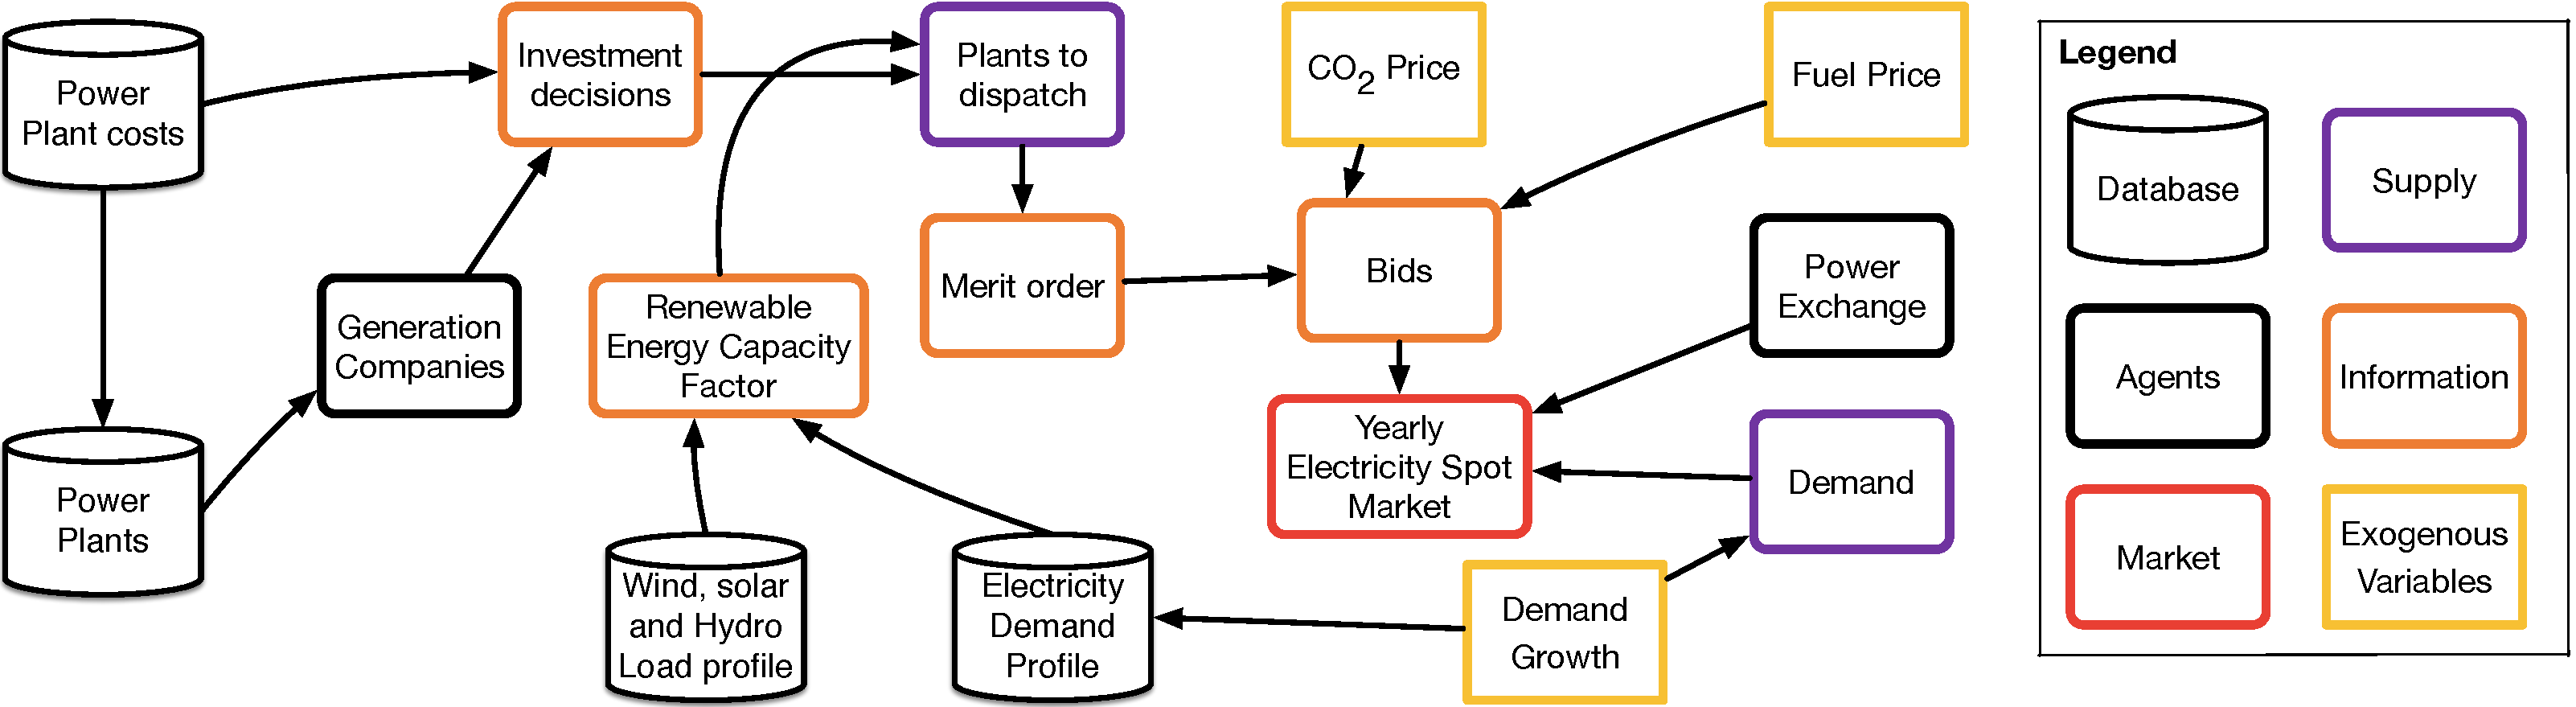
\includegraphics[width=\linewidth]{Chapter4/figures/low_level_system}
		\caption{ElecSim simulation overview}
		\label{fig:lowlevelsystem}
	\end{figure*}
\end{landscape}

Exogenous variables include fuel and \ce{CO2} prices as well as demand growth. Once the data is initialised, the world calls on the Power Exchange to operate the yearly electricity spot market. The world also settles the accounts of the GenCos, by paying bids, and removing operating and capital costs as well as loans and dividends.

%The world contains the functionality to dismantle old plants once they have reached the end of their lifetime. Power plants are taken out of service if they have not sold any electricity in the past 7 years, which is configurable in the configuration file. We decided upon this due to the fact that power generators have high, sunk capital costs, which often have high demolition costs. We assume, therefore, that generator companies are willing to wait circa $\frac{1}{4}$ of their lives to see if a pay-out occurs due to the breakdown of competing power plants, increasing demand, or governmental support in the form of a carbon tax increase or reduction.






%GenCos  invest in power plants based on the highest positive net present value (NPV). Bids are made for each power plant based on the power plants short run marginal cost. A Power Exchange operator matches these bids with demand in merit order. 



%\begin{figure}[h]
%	\begin{center}
%		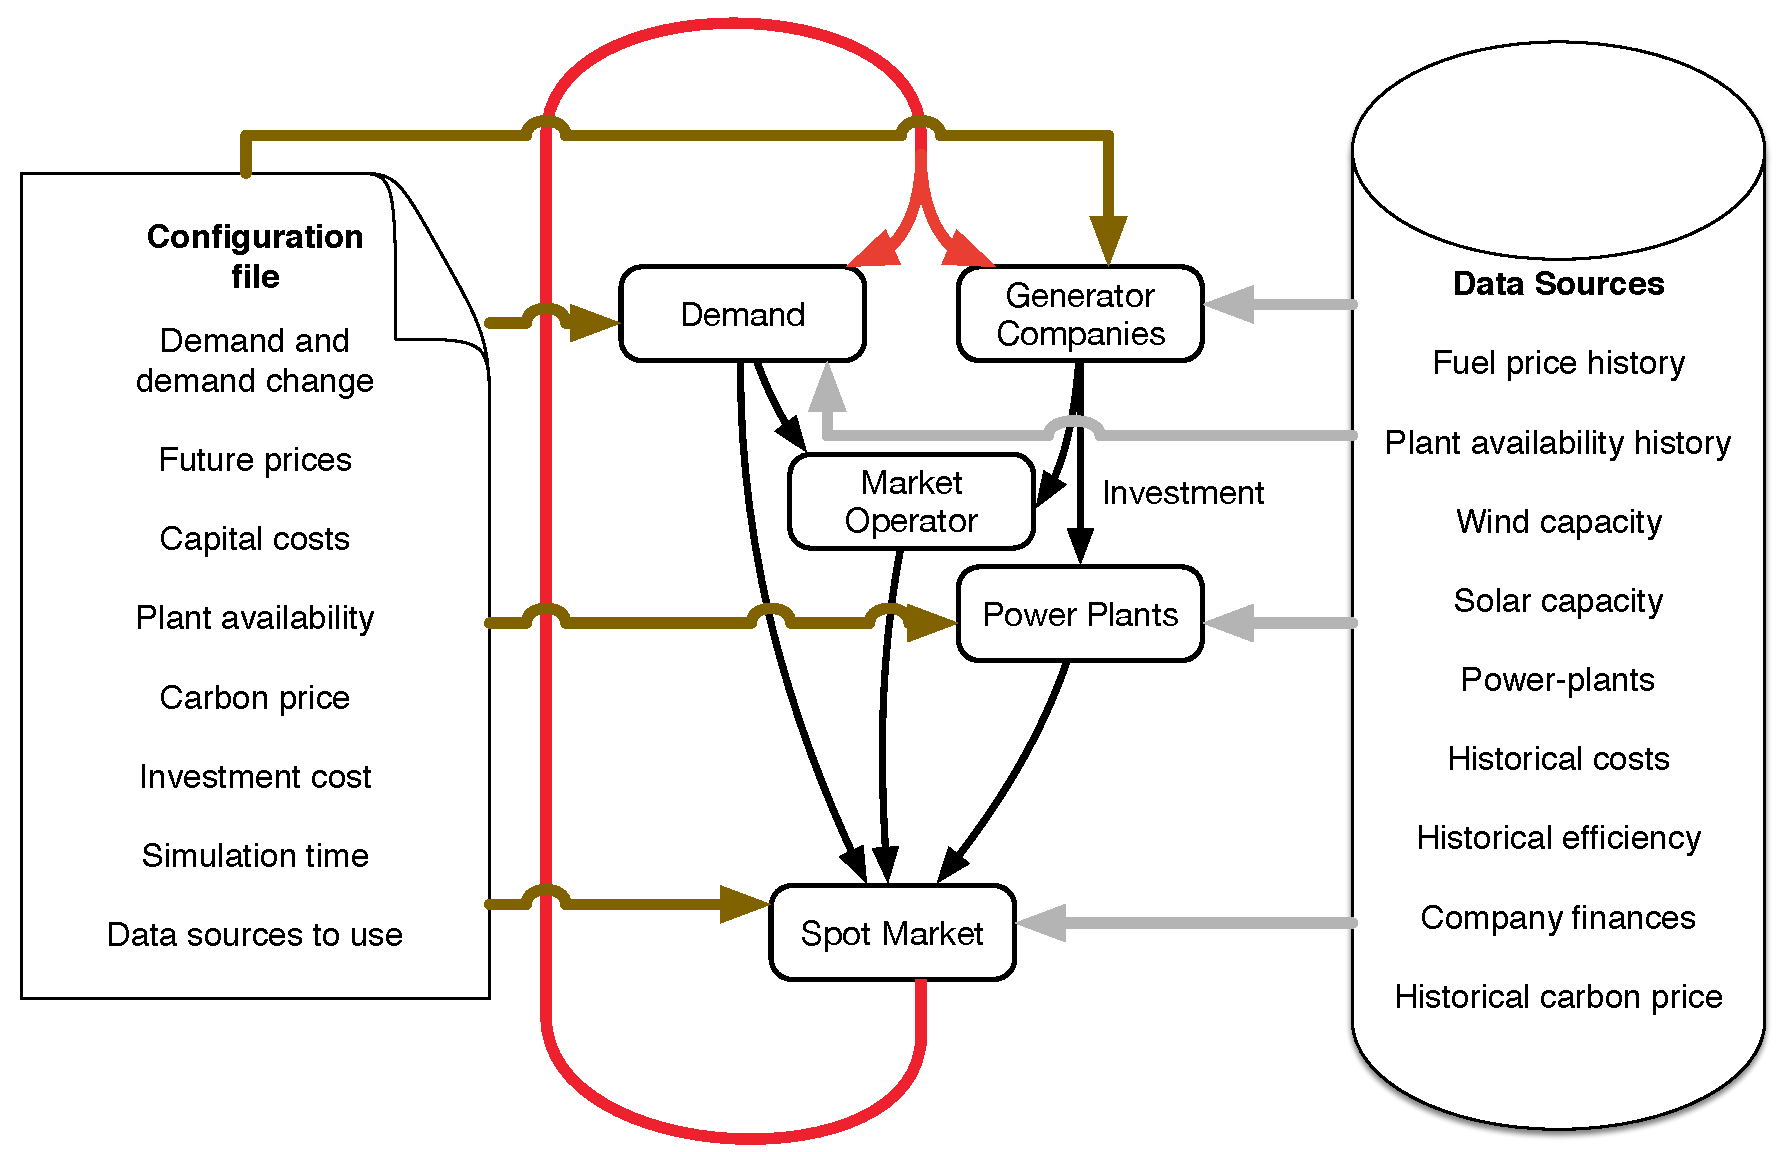
\includegraphics[width=0.5\textwidth]{figures/System_overview.pdf}
%		\caption{ElecSim simulation overview.}
%		\label{fig:system_overview}
%	\end{center}
%\end{figure}



% {\color{blue}
% \subsection{UK Case Study}

% Here we study a realisation of ElecSim, which we calibrated to the United Kingdom.

% \subsubsection{Exogenous Inputs}

% To model variance in gas and coal prices we used data from \cite{coalprices,gasprices}. Calibration of the load duration curve was taken from \cite{gbnationalgridstatus_2019}.

% Historical EU ETS carbon price was taken from \cite{jones_moore_macdonald_macdonald_buckley_macdonald_2019}. The EU ETS is the EU emissions trading scheme, which limits total carbon emissions within the EU area.

% \subsubsection{Power Plant Parameters}

% ElecSim's power generation costs are initialised using the UK government Department for Business, Energy and Industrial Strategy (BEIS) power plant generation report \cite{Department2016}. This contains information on power plants found in Table \ref{table:parameter_notation}.

% For historical power plants, we used historical costs of Levelised Cost of Energy (LCOE) \cite{Dale2013}, from the International Energy Agency and International Renewable Energy Agency energy cost reports, localised to the UK \cite{IEA2015,IRENA2018}. In this realisation, each parameter was scaled linearly going from the modern LCOE calculated from the BEIS report, to attain the relevant historical LCOE. Historical plant efficiency was taken into account for gas and coal power plants using data from the USA \cite{EIA2013}.

% Outages are modelled by using availability data of gas, coal, photovoltaic, offshore and onshore power generators \cite{Ltd2016, Hunt2015, carroll-j}. Historical availabilities are modelled for older gas, coal and hydro power plants \cite{AlbertaSystemElectricOperator2016}.

% Capacity factors were taken as an average of the UK for solar and wind \cite{Pfenninger2016, Staffell2016}.






% \subsubsection{Spot Market}

% The lost load is set to be \textsterling6000 to encourage investment as per the recommendations of the UK government \cite{DECC2013}.

% \subsubsection{Investment}

% As agents are modelled to have imperfect information, we model that they make predictions on future electricity and \ce{CO2} prices, as well as demand change. Each generation company has a different look-back period sampled uniformly from the previous 3 to 7 years.


% The cost of equity and debt is modelled as a weighted average cost of capital (WACC), with values of 5.9\% for non-nuclear power plants, and 10\% for nuclear power plants \cite{KPMG2017, Paper2012}. 

% }



%
%\begin{itemize}
%	\item Model can be modified through a single python scenario file which includes exogenous variables such as number of generation companies, power plants, power plant costs, tax and fuel prices, and demand.
%	\item Architectural framework:
%	\begin{itemize}
%		\item Agents are generation companies.
%		\item Generation companies initialized from government data. And randomized discount rate around a mean of 10\% for nuclear power plants and 5.9\% for other types of generators.
%		\item Costs of power plants taken from empirical data. 
%		\item Historical LCOE costs taken from data, with individual costs such as fixed operation and maintenance, construction and pre-development costs scaled linearly to match LCOE value. (This can be changed by user by specifying linear optimisation constraints).
%		\item Historical Gas turbine and Coal plant efficiency taken from epa data.
%		\item Variable operation and maintenance costs are stochastic to take into account differences in design types, preventative and corrective maintenance, labour costs and skill, asset and site management, health and safety and chance.
%		\item Electricity demand taken from historical data and split up into 19 load segments.
%		\item CO2 prices, fuel Prices, demand growth are exogenous
%		\item Fuel is bought by power producers each year at different prices, related to the standard deviation from historical data. This simulates different hedging strategies, luck and timing of fuel purchasing.
%		\item Outages are modelled by assuming a 93\% outage rate for fuel plants \cite{Ltd2016} and 97\% outage for renewables. \cite{carroll-j}
%		\item Generation companies bid their short run marginal costs.
%		\item Investments made on highest Net Present Value results. CO2 price, fuel price and demand are predicted 7 years ahead using linear regression. 
%		\item Estimated sale of electricity price calculated by simulating a market 7 years into the future with expected power plants that are running and have been taken out of service.
%		\item Investors will only invest if they have 25\% of the total upfront costs. (the rest taken on by debt and equity as assumed by WACC value.)
%		\item Intermittent power generators can only submit a certain percentage of their total capacity for each load segment. This percentage is matched with empirical data.
%		\item Bids accepted by a centralised Power Exchange based on merit order. Generation companies bid their short run marginal cost.
%	\end{itemize}
%	\item Assumptions: 
%	\begin{itemize}
%		\item Yearly time step
%		\item Renewables contribute to load curve of each demand segment matched with empirical data of typical wind and solar availability at each demand segment
%		\item Different discount rates per user (randomized)
%		\item Country initialized with full amount of power plants and generation companies in country and total demand data considered
%		\item No curtailment of renewables
%		\item Imperfect foresight - Prediction required for demand, co2 price, fuel cost, other investments.
%		\item Power plant construction and pre-development periods and costs modelled from UK Government BEIS data
%		\item Investments based on highest NPV using a single year 7 (can be changed in scenario file) time steps into the future to predict all years of power plant.
%		\item Agents predict next year's fuel, carbon and demand using linear regression and randomized look back period (between 3 and 6.)
%		\item Plants are dismantled after their lifetime, and only enter operation after pre-development/construction.
%		\item Legacy power plants are reinitialized to random starting year to account for refurbishment.
%		\end{itemize}
%\end{itemize}


%%%%%%%%%%%%%%%%%%%%%%%%%%%%%%%%%%%%%%%%%%%%%%%%
%%%%%%%%%%%%%%%%%%%%%%%%     Poster    %%%%%%%%%%%%%%%%
%%%%%%%%%%%%%%%%%%%%%%%%%%%%%%%%%%%%%%%%%%%%%%%%



We initialise the United Kingdom with our model with exemplar data from the UK. We model every single power plant in operation in the year 2018, which are owned by their respective generation companies. Individual historical power plant costs are estimated from levelized cost of electricity (LCOE) \cite{Dale2013, IEA2015,IRENA2018}, whereas future and present power plant costs are taken from the department of business and industrial strategy \cite{Department2016}. The variable operation and maintenance cost was defined stochastically to model the varying costs per project. A uniform distribution was chosen to provide sufficient variance between projects.

The demand agent is modelled as a single aggregated demand, split up into 20 segments of a yearly load duration curve (LDC), enabling us to increase speed of computation whilst maintaining accuracy. An LDC is defined as load sorted in order of magnitude. 

We model the influence of outages using availability data for gas, coal, photovoltaic, and wind power generators \cite{Ltd2016, Hunt2015, carroll-j}. Historical availabilities are modelled for old gas, coal and hydro power plants \cite{AlbertaSystemElectricOperator2016}. Capacity factors per geographical location were taken as an average of the UK for solar and wind \cite{Pfenninger2016, Staffell2016}. Where a capacity factor is defined as the ratio of electrical output over a given time period over the maximum possible electrical energy output. 

The generation companies make electricity bids each year for each of their power plants. The market operator then matches demand with supply in order of price, also known as merit-order dispatch. We model a uniform pricing market, where each of the companies are paid the highest accepted bid per load segment.

GenCos have the ability to invest every year in new power plants based on the expected net present value (NPV) of each type of power plant. NPV is a summation of the present value of a series of present and future cash flow. The NPV calculation is dependent on a stochastic representation of GenCos predictions of fuel, carbon and electricity price and demand.

Each GenCo has a separate weighted average cost of capital (WACC), which is the average rate that a company is expected to for its stock and debt. This is used as the discount rate in the NPV calculation \cite{KincheloeStephenC1990TWAC}. The WACC is modelled as a stochastic variable, with a Gaussian distribution, with a $\pm3\%$ standard deviation, with values of 5.9\% for non-nuclear power plants, and 10\% for nuclear power plants \cite{KPMG2017, Paper2012}. 

Stochasticity of fuel price within a year was also modelled, to take into account difference in hedging strategies and chance. An ARIMA model \cite{ARIMA} was fit to historic coal and natural gas prices.



%%%%%%%%%%%%%%%%%%%%%%%%%%%%%%%%%%%%%%%%%%%%%%%%
%%%%%%%%%%%%%%%%%%%%%%%%      Paper 2    %%%%%%%%%%%%%%%%
%%%%%%%%%%%%%%%%%%%%%%%%%%%%%%%%%%%%%%%%%%%%%%%%

\subsection{Representative days}
\label{elecsim:sec:representative}


In this subsection we describe how we decide the granularity of time-steps. Specifically, we use representative days. Representative days, in this context, are a subset of days which when scaled up to 365 days can adequately represent a year. 

In this paper, we initialised the model to a scenario of the United Kingdom as an example, however, the fundamental dynamics of the model remain the same for other decentralised electricity markets.


%\subsection{Representative Days}
%\label{ssec:representative_days}

%In previously published work, ElecSim modelled a single year as 20 time-steps for solar irradiance, onshore and offshore wind and electricity demand~\cite{Kell}. Similarly to findings of other authors, this relatively low number of time-steps led to an overestimation of the uptake of intermittent renewable energy resources (IRES) and an underestimation of flexible technologies~\cite{Ludig2011,Haydt2011}. This is due to the fact that the full intermittent nature of renewable energy could not be accurately modelled in such a small number of time-steps.



Similarly to findings of other authors, using a relatively low number of time-steps leads to an overestimation of the uptake of intermittent renewable energy resources (IRES) and an underestimation of flexible technologies~\cite{Ludig2011,Haydt2011}. This is due to the fact that the full intermittent nature of renewable energy could not be accurately modelled in such a small number of time-steps. 


To address this problem, whilst maintaining a tractable execution time, we approximated a single year as a subset of proportionally weighted, representative days. This enabled us to reduce computation time. Each representative day consisted of 24 equally separated time-steps, which model hours in a day. Hourly data was chosen, as this was the highest resolution of the dataset available for offshore and  onshore wind and solar irradiance \cite{Pfenninger2016}. A lower resolution would allow us to model more days, however, we would lose accuracy in terms of the variability of the renewable energy sources. 


Similarly to Nahmmacher \textit{et al.} we used a clustering technique to split similar days of weather and electricity demand into separate groups. We then selected the historic day that was closest to the centre of the cluster, known as the medoid, as well as the average of the centre, known as the centroid ~\cite{Nahmmacher2016}. Similarly to Nahmmacher, we used Ward's clustering algorithm and selected the centroid \cite{doi:10.1080/01621459.1963.10500845}. However, we also used the $k$-means clustering algorithm~\cite{forgy65}. This was due to the ability for the $k$-means algorithm to cluster time-series into relevant groups \cite{Kell2018}. These days were scaled proportionally to the number of days within their respective cluster to approximate a total of 365 days.

Equation \ref{elecsim:eq:medoids_series} shows the series for a medoid or centroid, selected by the clustering algorithms:

\begin{equation}
\label{elecsim:eq:medoids_series}
P^{x,i}_{h}=\{P_1, P_2, \ldots, P_{24}\}
\end{equation}

\noindent where $P^{x,i}_{h}$ is the medoid for series $x$, where $x\in X$ refers to offshore wind capacity factor, onshore wind capacity factor, solar capacity factor and electricity demand, $h$ is the hour of the day and $i$ is the respective cluster. $\{P_1, P_2, \ldots , P_{24}\}$ refers to the capacity values at each hour of the representative day.

We then calculated the weight of each cluster. This gave us a method of assigning the relative importance of each representative day when scaling the representative days up to a year. The weight is calculated by the proportion of days in each cluster. This gives us a method of determining how many days within a year are similar to the selected medoid or centroid. The calculation for the weight of each cluster is shown by Equation \ref{elecsim:eq:cluster_weight}:

\begin{equation}
\label{elecsim:eq:cluster_weight}
w_i = \frac{n_i}{||N||} 
\end{equation} 

\noindent where $w_i$ is the weight of cluster $i$, $n_i$ is the number of days in cluster $i$, and $||N||$ is the total number of days that have been used for clustering. 


The next step was to scale up the representative days to represent the duration curve of a full year. We achieved this by using the weight of each cluster, $w_i$, to increase the number of hours that each capacity factor contributed in a full year. Equation \ref{elecsim:eq:scaled-medoid} details the scaling process to turn the medoid or centroid, shown in Equation \ref{elecsim:eq:medoids_series}, into a scaled day. Where $\widetilde{P}^{x,i}_{h}$ is the scaled day:

\begin{equation}
\label{elecsim:eq:scaled-medoid}
\widetilde{P}^{x,i}_{h} =  \{P_{1w_i}, P_{2w_i}, \ldots, P_{24w_i}\}
\end{equation} 

\noindent Equation \ref{elecsim:eq:scaled-medoid} effectively extends the length of the day proportional to the amount of days in the respective cluster.


%The total time series for series $x$ is shown by Equation \ref{eq:total_time_series}

Finally, each of the scaled representative days were concatenated to create the series used for the calculations which required the capacity factors and the respective number of hours that each capacity factor contributed to the year. Equation \ref{elecsim:eq:total_time_series} displays the total time series for series $x$, where each scaled medoid is concatenated to produce an approximated time series, $\widetilde{P}^x$:


\begin{equation}
\label{elecsim:eq:total_time_series}
\widetilde{P}^x=\left(\widetilde{P}^{x,1}_{h},\widetilde{P}^{x,2}_{h},\ldots, \widetilde{P}^{x,||N||}_{h}\right)
\end{equation}

\noindent the total number of hours in the approximated time series, $\widetilde{P}^x$, is equal to the number of hours in a day multiplied by the number of days in a year, which gives the total number of hours in a year ($24\times 365=8760$), as shown by Equation \ref{elecsim:eq:total_scale}:


\begin{equation}
\label{elecsim:total_scale}
\sum\limits_{w\in W}\sum\limits_{t=1}^{T=24}\left(w_i t\right)=24\times 365=8760
\end{equation}

\noindent where $w\in W$ is the set of clusters.

\subsection{Error Metrics}

To measure the validity of our approximation using representative days and also compare the optimum number of days, or clusters, we used a technique similar to Poncelet \textit{et al.} \cite{Dhaeseleer2015, Poncelet2017}. We trialled the number of clusters against three different metrics: correlation ($CE_{av}$), normalised root mean squared error ($nRMSE$) and relative energy error ($REE_{av}$). 

$REE_{av}$ is the average value over all the considered time series $\widetilde{P}^x{\in} \widetilde{P}$ compared to the observed average value of the set $P^x\in P$. Where $P^x\in P$ are the observed time series and $\widetilde{P}^x{\in} \widetilde{P}$ are the scaled, approximated time series using representative days. $REE_{av}$ is shown formally by Equation \ref{eq:ree_av}:


\begin{equation}
\label{eq:ree_av}
REE_{av}=\frac
{\sum\limits_{P^x{\in} P}\left(\left|
	\frac
	{\sum\limits_{t\in T}DC_{P^x_t}-\sum\limits_{t\in T}\widetilde{DC}_{\widetilde{P}^x_t}}
	{\sum\limits_{t\in T}DC_{P^x_t}}
	\right|\right)
}
{\left|\left|P\right|\right|}
\end{equation}

\noindent where $DC_{P^x_t}$ is the duration curve for $P^x$ and $DC_{\widetilde{P}^x_t}$ is the duration curve for $\widetilde{P}^x$. In this context, the duration curve can be constructed by sorting the capacity factor and electrical load data from high to low. The $x-$axis for the DC exhibits the proportion of time that each capacity factor represents. The approximation of the duration curve is represented in this text as $\widetilde{DC}_{\widetilde{p}^x}$.

$t\in T$ refers to a specific time step of the original time series. $\widetilde{DC}$ refers to the approximated duration curve for $\widetilde{P}^x$. Note that in this text $\left|\cdot\right|$ refers to the absolute value, and $\left|\left|\cdot\right|\right|$ refers to the cardinality of a set and $\left|\left|P\right|\right|$ refers to the total number of of considered time series.

Specifically, the sum of the observed values, $P^x$, and approximated values, $\widetilde P^x$, for all of the time series are summed. The proportional difference is found, which is summed for each of the different series, $x$, and divided by the number of series, to give $REE_{av}$.





%$nRMSE$ is measured as the normalised root mean squared error between the actual duration curve and representative duration curve, $DC$.  

%Another metric that we wanted to measure was that of the distribution of electricity demand and capacity factors to be similar to that of the actual time series. The distribution can be represented by a duration curve ($DC$) of the original time series. We therefore used the normalised root mean squared error between the actual duration curve and representative duration curve. 

Another requirement is for the distribution of load and capacity factors for the approximated series to correspond to the observed time series. It is crucial that we can account for both high and low levels of demand and capacity factor for IRES generation. This enables us to model for times where flexible generation capacity is required.

The distribution of values can be represented by the duration curve ($DC$) of the time series. Therefore, the average normalised root-mean-square error ($NRMSE_{av}$) between each $DC$ is used as an additional metric. The $NRMSE_{av}$ is shown formally by Equation \ref{eq:nrmse_av}:

\begin{equation}
\label{eq:nrmse_av}
NRMSE_{av}=\frac
{\sum\limits_{P^x{\in} P}\left(\frac
	{\sqrt{
			\frac{1}{\left|\left|T\right|\right|}
			\cdot
			\sum\limits_{t\in T}(DC_{P^x_t}-\widetilde{DC}_{\widetilde{P}^x_t})^2}
	}
	{max(DC_{P^x})-min(DC_{P^x})}
	\right)}
{\left|\left|P\right|\right|}.
\end{equation}

Specifically, the difference between the approximated and observed duration curves for each time-step $t$ is calculated. The average value is then taken of these differences. This average value is then normalised for the respective time series $P^x$. The average of these average normalised values for each time series are then taken to provide a single metric, $NRMSE_{av}$.



The final metric used is the correlation between the different time series. This is used due to the fact that wind and solar output influences the load within a single region, solar and wind output are correlated, as well as offshore and onshore wind levels within the UK. This is referred to as the average correlation error ($CE_{av}$) and shown formally by Equation \ref{eq:ce_av}:


\begin{equation}
\label{eq:ce_av}
CE_{av}=\frac{2}{\left|\left|P\right|\right|\cdot(\left|\left|P\right|\right|-1)}\cdot
\left(
\sum\limits_{p_i\in P}\sum\limits_{p_j\in P,j>i}
\left|
corr_{p_i,p_j}-\widetilde{corr}_{p_i,p_j}
\right|
\right)
\end{equation}

\noindent where $corr_{p1,p2}$ is the Pearson correlation coefficient between two time series $p_1,p_2\in P$, shown by Equation \ref{eq:corr}. Here, $V_{p1,t}$ represents the value of time series $p_1$ at time step t:

\begin{equation}
\label{eq:corr}
corr_{p1,p2}=\frac
{\sum\limits_{t\in T}\left(\left(V_{p1,t}-\overline{V}_{p1}\right)\cdot\left(V_{p2,t}-\overline{V}_{p2}\right)\right)}
{\sqrt{
		\sum\limits_{t\in T} \left(V_{p_1,t}-\overline{V}_{p1}\right)^2\cdot\sum\limits_{t\in T}\left(V_{p2,t}-\overline{V}_{p2}\right)^2
}}.
\end{equation}


%We found that for each of these metrics, the accuracy of the approximation did not significantly increase after 8 days. We therefore selected 8 days as a compromise between accuracy and tractability for the model.











%Firstly, the average capacity factor over the selected time series should preserve the annual electricity demand load factors. To evaluate the ability for the representative days, the average value over all the considered time series $p\in P$ compared to the actual average value is used as a metric. This is referred to as $REE_{av}$. Note that in this text $\left|\cdot\right|$ refers to the absolute value and $\left|\left|\cdot\right|\right|$ refers to the cardinality of a set. Below, the index $t\in T$ refers to a specific time step of the original time series (e.g. hourly interval).
%
%\begin{equation}
%	REE_{av}=\frac
%	{\sum\limits_{p\in P}\left(\left|
%	\frac
%	{\sum\limits_{t\in T}DC_{p,t}-\sum\limits_{t\in T}\widetilde{DC}_{p,t}}
%	{\sum\limits_{t\in T}DC_{p,t}}
%	\right|\right)
%	}
%	{\left|\left|P\right|\right|}
%\end{equation}
%
%Another metric that we wanted to measure was that of the distribution of electricity demand and capacity factors to be similar to that of the actual time series. The distribution can be represented by a duration curve ($DC$) of the original time series. We therefore used the normalised root mean squared error between the actual duration curve and representative duration curve. In this context, the duration curve can be constructed by sorting the capacity factor and electrical load data from high to low. The $x-$axis for the DC exhibits the proportion of time that each capacity factor represents. The approximation of the duration curve is represented in this text as $\widetilde{DC}_p$.
%
%%\begin{equation}
%%	NRMSE_{av}=\frac
%%	{\sum\limits_{p\in P}\left(
%%	\frac{\sqrt{\frac{1}{\left|\left|T\right|\right|}}\cdot \sum\limits_{t\in T}
%%	\left(
%%	DC_{p,t}-\widetilde{DC}_{p,t}
%%	\right)^2}{max(DC_p)-min(DC_p)}}
%%	\right
%%	}
%%	{\left|\left|P\right|\right|}
%%\end{equation}
%
%%\begin{equation}
%%	NRMSE_{av}=\frac
%%	{\sum\limits_{p\in P}\left(\frac
%%	{
%%	\sqrt{
%%	\frac{1}{\left|\left|T\right|\right|}
%%	\cdot
%%	\sum\limits_{t\in T}
%%	\left(
%%	DC_{p,t}-\widetilde{DC}_{p,t}
%%	\right)^2
%%	}
%%	}
%%	{max(DC_p)-min(DC_p)\right)}
%%	}{
%%	\left|\left|P\right|\right|
%%	}
%%\end{equation}
%
%\begin{equation}
%	NRMSE_{av}=\frac
%	{\sum\limits_{p\in P}\left(\frac
%	{\sqrt{
%	\frac{1}{\left|\left|T\right|\right|}
%	\cdot
%	\sum\limits_{t\in T}(DC_{p,t}-\widetilde{DC}_{p,t})^2}
%	}
%	{max(DC_p)-min(DC_p)}
%	\right)}
%	{\left|\left|P\right|\right|}
%\end{equation}
%
%
%The final metric used is the correlation between the different time series. This is used due to the fact that wind and solar output influences the load within a single region. This is referred to as the average correlation error ($CE_{av}$).
%
%\begin{equation}
%	CE_{av}=\frac{2}{\left|\left|P\right|\right|\cdot(\left|\left|P\right|\right|-1)}\cdot
%	\left(
%	\sum\limits_{p_i\in P}\sum\limits_{p_j\in P,j>i}
%	\left|
%	corr_{p_i,p_j}-\widetilde{corr}_{p_i,p_j}
%	\right|
%	\right)
%\end{equation}
%
%Where $corr_{p1,p2}$ is the Pearson correlation coefficient between two time series $p_1,p_2\in P$. Here, $V_{p1,t}$ represents the value of time series $p_1$ at time step t. 
%
%\begin{equation}
%	corr_{p1,p2}=\frac
%	{\sum\limits_{t\in T}\left(\left(V_{p1,t}-\overline{V}_{p1}\right)\cdot\left(V_{p2,t}-\overline{V}_{p2}\right)\right)}
%	{\sqrt{
%	\sum\limits_{t\in T} \left(V_{p_1,t}-\overline{V}_{p1}\right)^2\cdot\sum\limits_{t\in T}\left(V_{p2,t}-\overline{V}_{p2}\right)^2
%	}}
%\end{equation}
%
%Figure \ref{fig:clusters_compared} displays the number of clusters plot against each of the error metrics. For this experiment we chose eight clusters, due to eight being the smallest number with the best performing error metrics. After eight clusters $NRMSE_{av}$ and $CE_{av}$ do not improve significantly, whilst $REE_{av}$ deteriorates with number of clusters. Selecting less than eight clusters leads to a significant deterioration for both $CE_{av}$ and $NRMSE_{av}$.
%
%\begin{figure*}
%\centering
%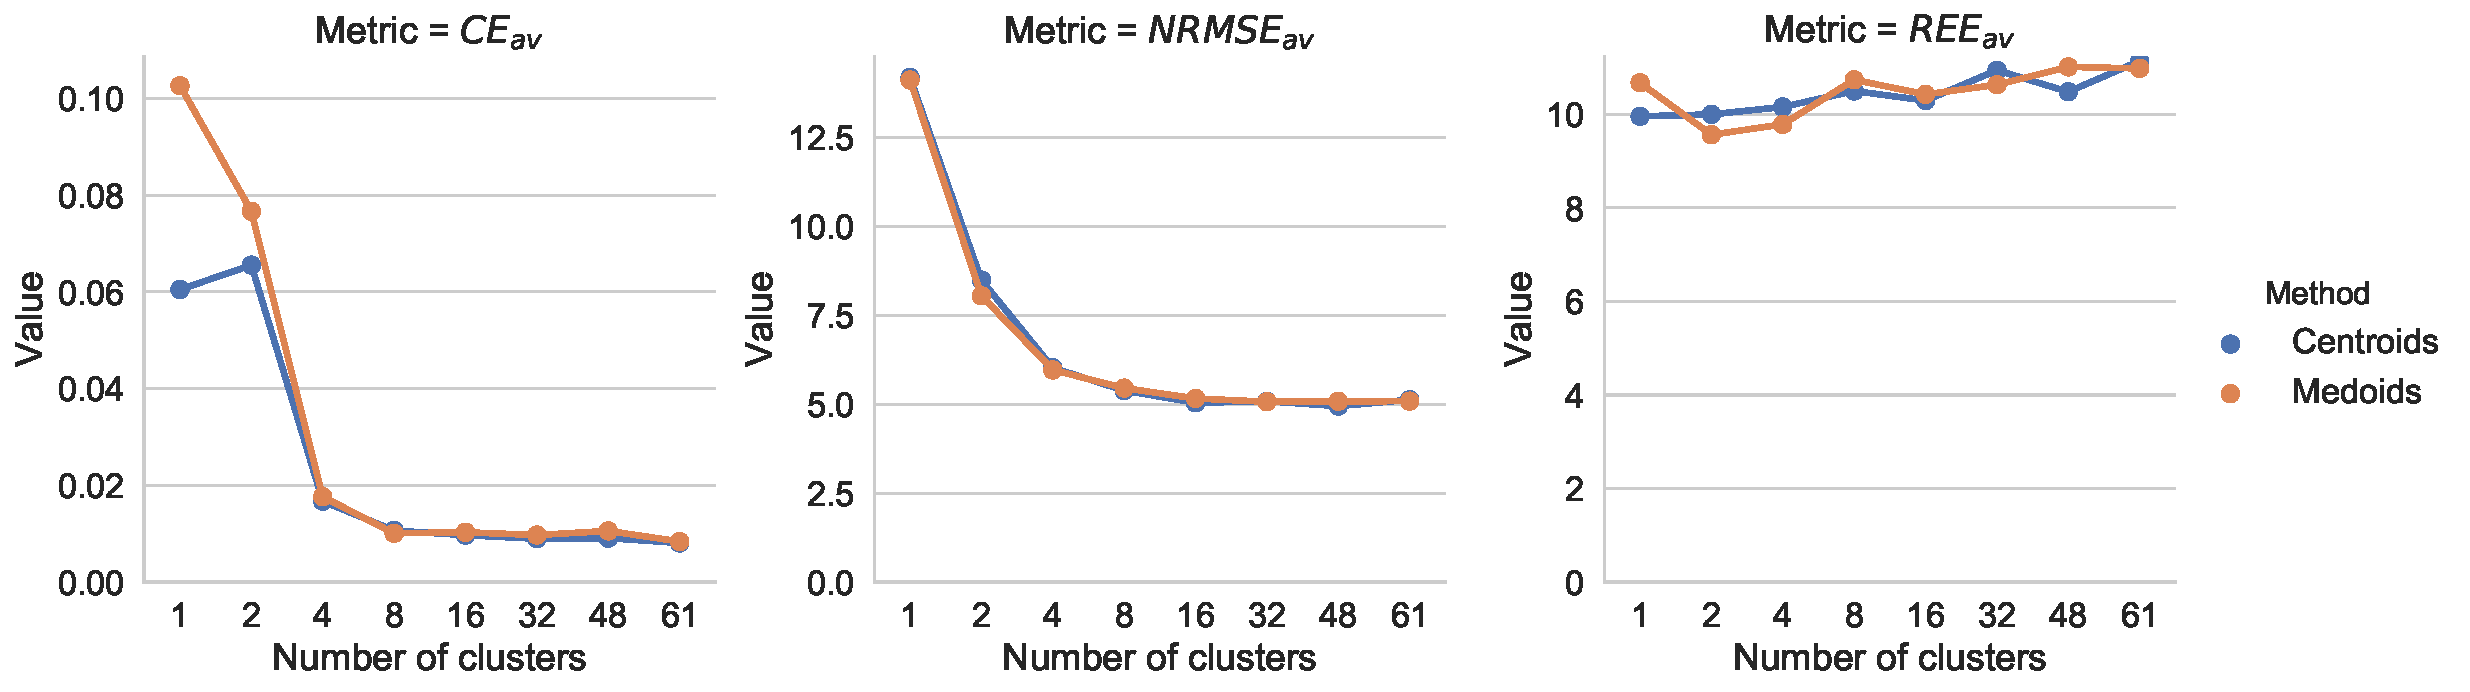
\includegraphics[width=\textwidth]{figures/methods_and_materials/clusters_compared.pdf}
%\caption{Comparison of number of clusters for accuracy.}
%\label{fig:clusters_compared}
%\end{figure*}
%
%The error metrics do not exhibit a significant difference between using either the centroids or medoids technique. However, we chose to use the medoids technique. This was done due to the fact that the extreme high and low values would not be lost due to averaging \cite{Hilbers2019}.
%
%Figure \ref{fig:clusters_compared_load} and Figure \ref{fig:clusters_compared_resources} display the resultant representative days that were used to represent an entire year in the simulation. A positive correlation between onshore and offshore wind speed can be seen in Figure \ref{fig:clusters_compared_resources}, which one would expect for the relatively small geography of the United Kingdom. Between the hours of 96 and 120 a negative correlation of solar irradiance and wind speed is exhibited, which may refer to a particularly sunny and windless day. Whereas between 72 and 96 a particularly windy and sunless day is exhibited.
%
%\begin{figure}
%\centering
%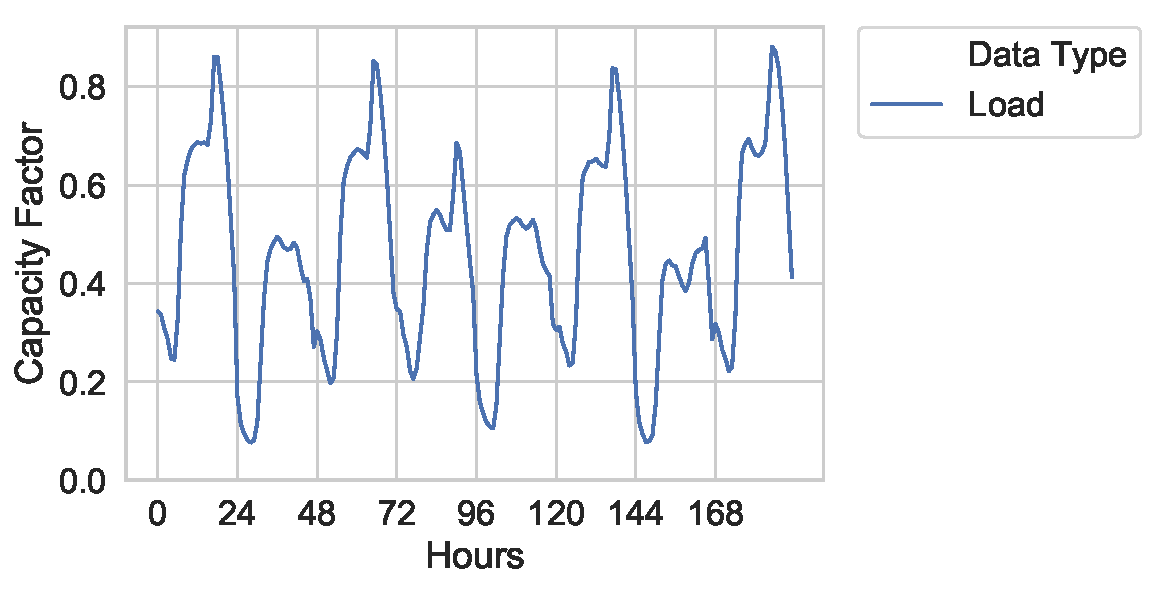
\includegraphics[width=0.49\textwidth]{figures/methods_and_materials/clusters_results_load.pdf}
%\caption{Representative days of electricity demand.}
%\label{fig:clusters_compared_load}
%\end{figure}
%
%Figure \ref{fig:clusters_compared_load} refers to the electrical load of the representative days. It should be noted that these representative days represent a quasi-temporal year and do not represent actual months.
%
%
%\begin{figure}
%\centering
%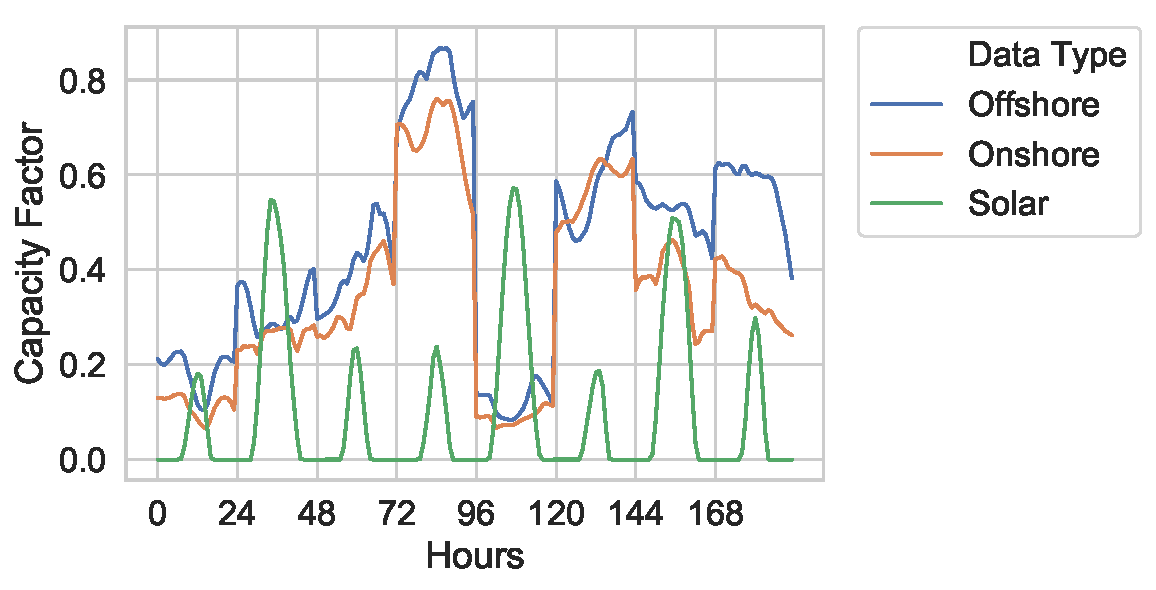
\includegraphics[width=0.49\textwidth]{figures/methods_and_materials/clusters_results_resources.pdf}
%\caption{Representative days of renewable resources.}
%\label{fig:clusters_compared_resources}
%\end{figure}


\subsubsection{Integrating higher temporal granularity}

To integrate the additional temporal granularity of the model, extra time-steps were taken per year. The higher temporal granularity of the model enabled us to accurately model the hourly fluctuations in solar and wind  which leads to more accurate expectations of the investment opportunities of these technologies ~\cite{Ludig2011,Haydt2011}.

GenCos make bids at the beginning of every time-step and the Power Exchange matches demand with supply in merit-order dispatch using a uniform pricing market. An example of electricity mix in a single representative day is shown in Figure \ref{fig:single_dispatched_day}. 

%
%\begin{equation}
%\label{eq:merit-order-dispatch}
%	\min_{b}
%	\sum\limits_{n=0}^{||b||}
%	\left(
%	b
%	\right)
%\end{equation}

Figure \ref{fig:single_dispatched_day} displays the high utilization of low marginal-cost generators such as nuclear, wind and photovoltaics. At hour 19, an increase in offshore wind leads to a direct decrease in CCGT. In contrast to this, a decrease in offshore and onshore between the hours of 8 and 12 lead to an increase in dispatch of coal and CCGT. One would expect this behaviour to prevent blackouts and meet demand at all times. This process has enabled us to more closely match fluctuations in IRES.

\begin{figure}
	\centering
	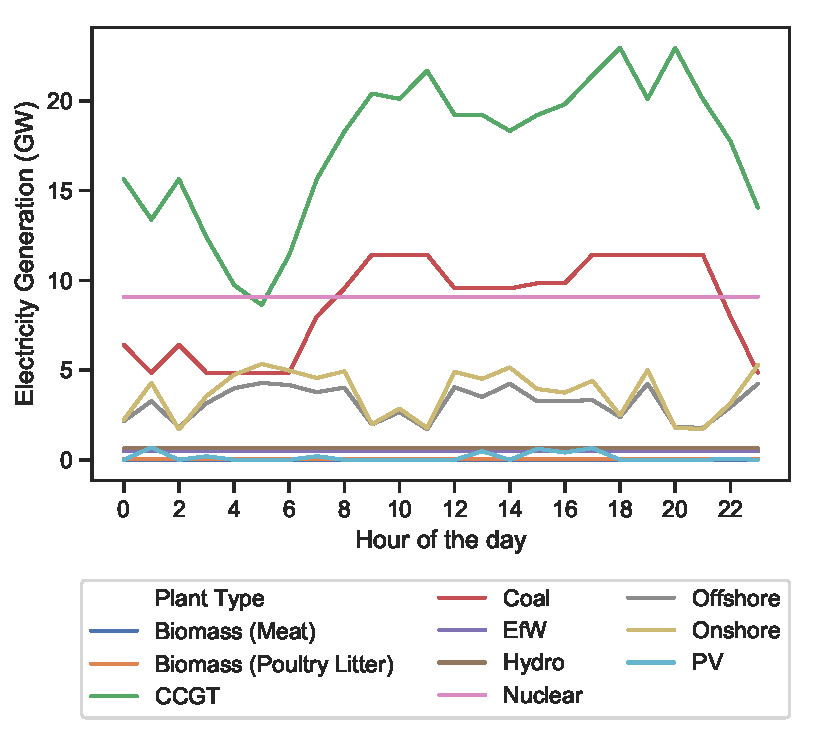
\includegraphics[width=0.7\textwidth]{Chapter4/figures/e-Energy-2020/methods_and_materials/clusters_results_single_day.pdf}
	\caption{Example of a single day of dispatched supply.}
	\label{fig:single_dispatched_day}
\end{figure}


\subsubsection{Evaluation of representative days}
\label{ssec:res_repr_days}

Figure \ref{fig:error_metrics_vs_cluster_number} displays the error metrics versus number of clusters. Both $CE_{av}$ and $NRMSE_{av}$ display similar behaviour for the $k$-means approach (centroids and medoids), namely the error improves significantly from a single cluster to eight clusters for both centroids and medoids. For the number of clusters greater than eight there are diminishing returns. For $REE_{av}$, however, the error metric is best at a single cluster, and gets worse with the number of clusters. The Wards approach, however, performs significantly worse for all metrics at every number of clusters. 



We chose eight clusters, for centroids and medoids, as a compromise between accuracy of the three error metrics and compute time of the simulation. This is because, eight was the largest number of clusters that gave us the lowest score for $CE_{av}$, $NRMSE_{av}$ and $REE_{av}$ without significantly increasing compute time. Whilst there was little significant difference between centroid and medoid, we chose to use the medoids due to the fact that the extreme high and low values would not be lost due to averaging \cite{Hilbers2019}.



%\begin{figure}
%	\centering
%	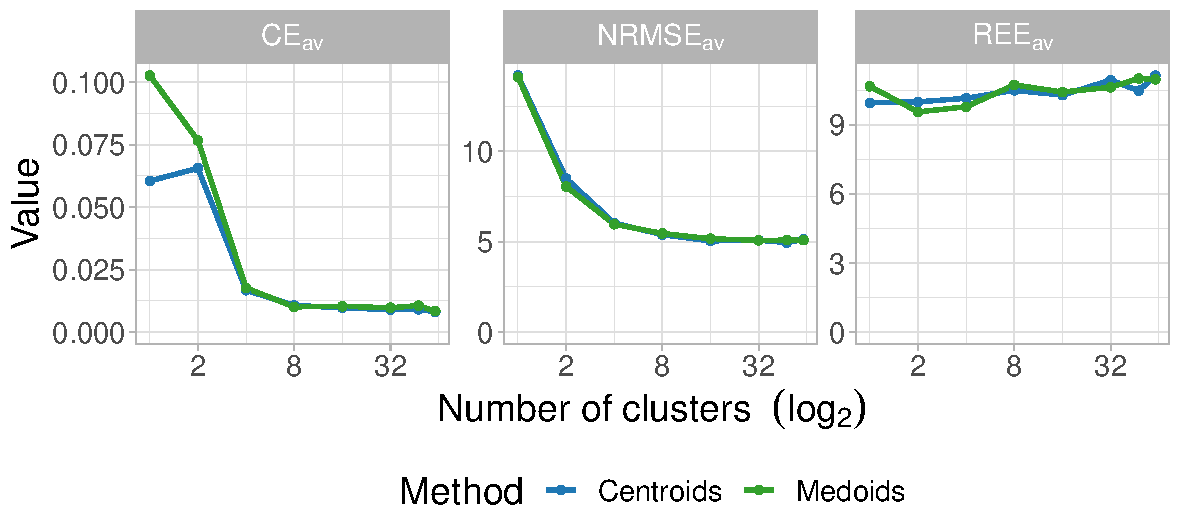
\includegraphics[width=0.8\textwidth]{Chapter4/figures/e-Energy-2020/methods_and_materials/clusters_compared_ggplot.pdf}
%	\caption{Number of clusters compared to error metrics.}
%	\label{fig:error_metrics_vs_cluster_number}
%\end{figure}


\begin{figure}
	\centering
	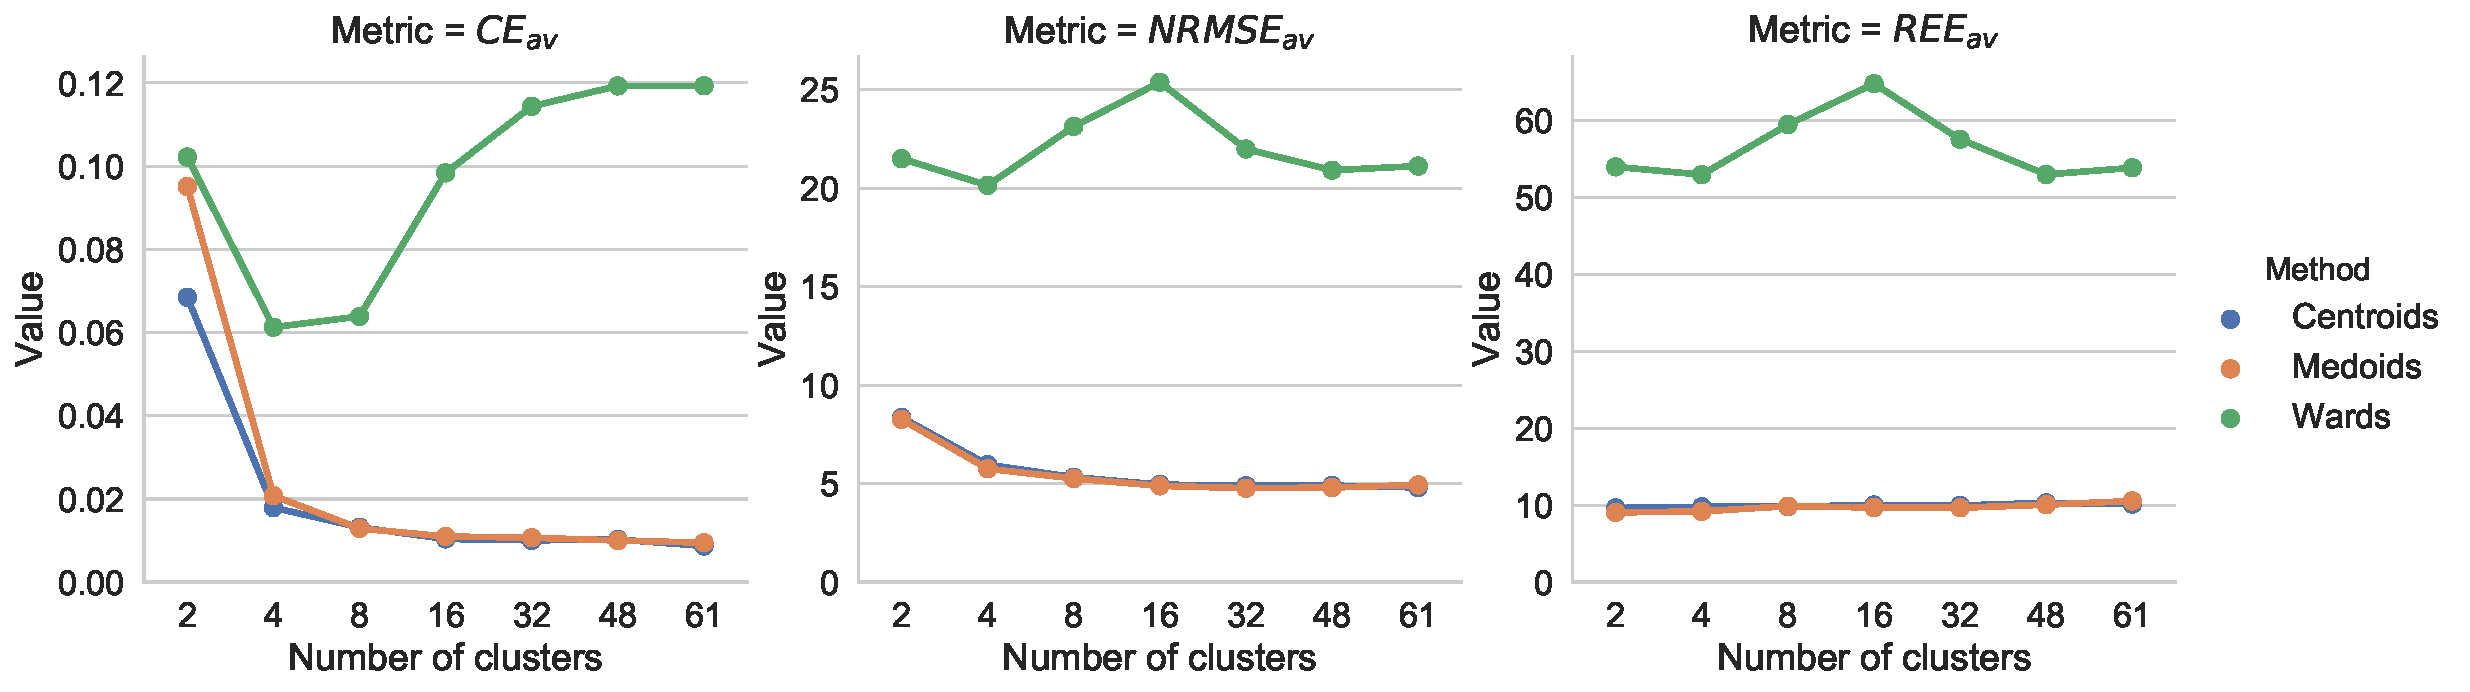
\includegraphics[width=0.9\textwidth]{Chapter4/figures/clusters_compared_wards.pdf}
	\caption{Number of clusters compared to error metrics.}
	\label{fig:error_metrics_vs_cluster_number}
\end{figure}





\section{Validation and performance}
\label{architecture:sec:validation}

In this section we detail the validation approaches taken in our model. For this, we take two approaches. One is to compare the price duration curve of the actual vs. our simulated price duration curve in 2018 using the 20 time-steps per year approach. The other is to use cross-validation between the years 2013 and 2018, using our representative days approach.


\subsection{Price Duration Curve Validation}

Validation of models is important to ascertain that the output is accurate. However, it should be noted that these long-term simulations are not predictions of the future, rather possible outcomes based upon certain assumptions. Jager posits that a certain outcome or development path, captured by empirical data, might have developed in a completely different direction due to chance. However, the processes that emerge from a model should be realistic and in keeping with expected behaviour \cite{Jager2006a}.

We begin by comparing the price duration curve in the year 2018. Figure \ref{fig:price_duration_curve} shows the N2EX Day Ahead Auction Prices of the UK \cite{nordpool_2019}, the Monte-Carlo simulated electricity prices, and the non Monte-Carlo electricity price throughout the year 2018. Fuel prices varying throughout a year, as does $V_C$ and WACC. WACC is sampled from a Gaussian distribution with a standard deviation of $\pm3$\%. $V_C$ is sampled from a uniform distribution between 30\% and 200\% of the mean $V_C$ price, whilst fuel price is sampled from the residuals of an ARIMA model fit on historical data. The N2EX Day Ahead Market is a day ahead market run by Nord Pool AS. Nord Pool AS runs the largest market for electrical energy in Europe, measured in volume traded and in market share \cite{nordpool_2019}.



\begin{figure}
	\begin{center}
		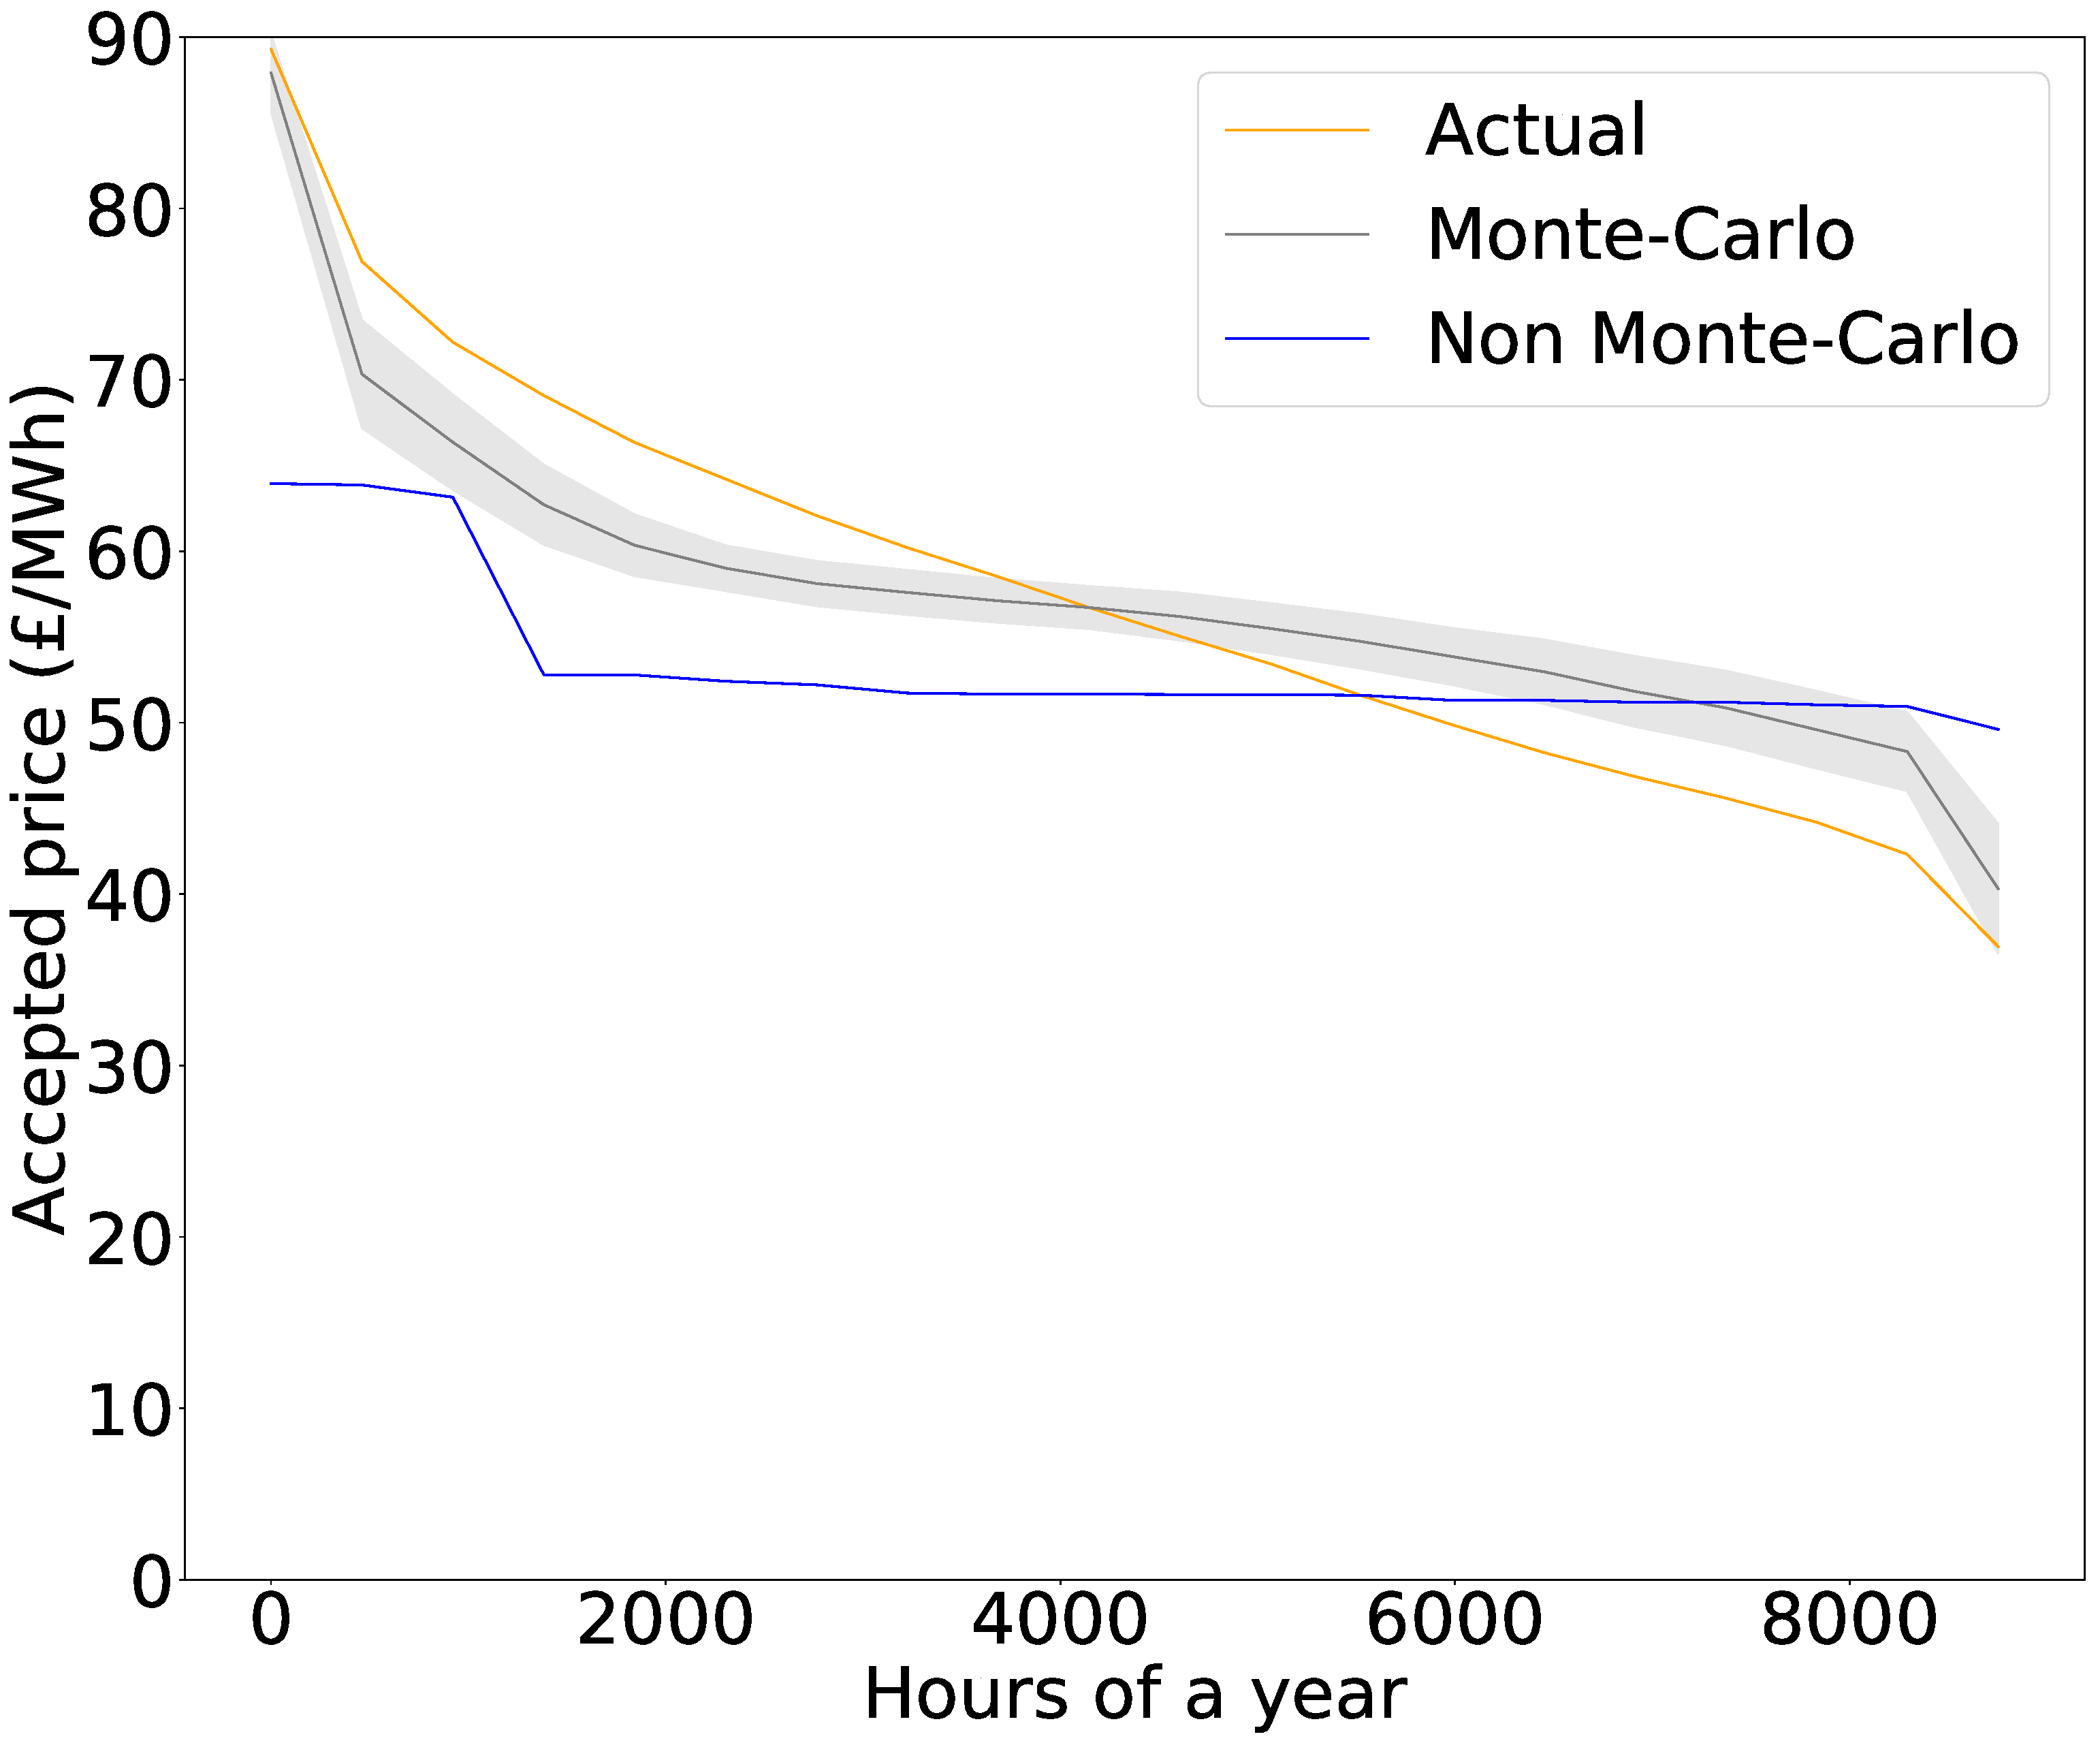
\includegraphics[width=0.6\textwidth]{Chapter4/figures/load_price_duration_curve_comparison-monte-carlo.pdf}
		\caption{Price duration curve which compares real electricity prices to those paid in ElecSim (2018).}
		\label{fig:price_duration_curve}
	\end{center}
\end{figure}

%\begin{table}
%	\centering
%	\csvautobooktabular{tables/validation/initialisation_run_validation.csv}
%	\caption{Validation performance metrics.}
%	\label{table:validation_metrics}
%\end{table}





We ran the initialisation of the model 40 times to capture the price variance. Outliers were removed as on a small number of occasions large jumps in prices at peak demand occurred which deviated from the mean. We did this, as although this does occur in real life, it occurs at a smaller fraction of the time than 5\% of the year (twenty time-steps per year), therefore the results would be unreasonably skewed for the highest demand segment. 

Figure \ref{fig:price_duration_curve} demonstrates very little variance in the non-stochastic case. This is due to the fact that combined cycle gas turbines (CCGTs) set the spot price. These CCGTs have little variance between one another as they were calibrated using the same dataset. By adding stochasticity of fuel prices and operation and maintenance prices, a curve that more closely resembles the actual data occurs. The stochastic curve, however, does not perfectly fit the real data, which may be due to higher variance in fuel prices and historical differences in operation and maintenance costs between power plants. One method of improving this would be fitting the data used to parametrise to the curve.

Table \ref{table:validation_metrics} shows performance metrics of the stochastic and non-stochastic runs versus the actual price duration curve . The stochastic implementation, improves the mean absolute error (MAE) of the non-stochastic case by $52.5\%$.

\begin{table}[]
	\begin{tabular}{p{4cm}p{4cm}p{2.5cm}p{3cm}}
		\hline
		Metric & N2EX Day Ahead & ElecSim & Non Monte-Carlo \\ \hline
		Avg. Price (\textsterling/MWh) & 57.49 & 57.52 & 53.39 \\
		Std. dev (\textsterling/MWh) & - & 9.64 & - \\
		MAE (\textsterling/MWh) & - & 3.97 & 8.35 \\
		RMSE (\textsterling/MWh) & - & 4.41 & 10.2 \\ \hline
	\end{tabular}
	\caption{Validation performance metrics.}
	\label{table:validation_metrics}
\end{table}

%By observing the processes that emerge from the long-term scenarios, we can see that carbon price and investment in renewable generation are positively correlated, as would be expected. The highest NPV calculations were for onshore wind and CCGT plants. This is realistic for the United Kingdom, where subsidies are required for other forms of generation such as coal and nuclear.



%%%%%%%%%%%%%%%%%%%%%%%%%%%%%%%%%%%%%%%%%%%%%%%%
%%%%%%%%%%%%%%%%%%%%%%%%      Paper 2    %%%%%%%%%%%%%%%%
%%%%%%%%%%%%%%%%%%%%%%%%%%%%%%%%%%%%%%%%%%%%%%%%


\subsection{Representative days validation}
\label{elecsim:ssec:representative_validation}

In this section we detail the approach taken in this paper to validate our model using representative days as time-steps. 

To achieve this, we use a genetic algorithm to find the predicted price duration curves which lead to the smallest error between our simulated electricity mix and the scenarios tested. The scenarios examined here are the observed electricity mix of the UK between 2013 and 2018 and the BEIS reference scenario projected in 2018 till 2035. When projecting the BEIS reference scenario we also optimise for nuclear subsidy and uncertainty in the price duration curves.


%For GenCos to adequately make investments, they must formulate an expectation of future electricity prices over the lifetime of a plant. For this paper, we use the net present value (NPV) metric to compare investments. 


%NPV provides a method for evaluating and comparing investments with cash flows spread over many years, making it suited for evaluating power plants which have a long lifetime.  

%Equation \ref{eq:npv_eq} is the calculation of NPV, where $t$ is the year of the cash flow, $i$ is the discount rate, $N$ is the total number of years, or lifetime of power plant, and $R_t$ is the net cash flow of the year $t$.
%\begin{equation} \label{eq:npv_eq}
%NPV(i, N) = \sum_{t=0}^{N}\frac{R_t}{(1+t)^t}
%\end{equation}

As mentioned in Section \ref{elecsim:sec:architecture}, GenCos make investments based upon the net present value. As shown in Equation \ref{architecture:eq:npv_eq}, an expectation of the net cash flow, $R_t$ is required. 

The net cash flow, $R_t$, is calculated by subtracting both the operational and capital costs from revenue over the expected lifetime of the prospective plant. The revenue gained by each prospective plant is the expected price they will gain per expected quantity of MWh sold over the expected lifetime of the plant. This is shown formally in Equation \ref{eq:revenue_total}:


\begin{equation}
\label{eq:revenue_total}
R_t = 
\sum\limits_{t=0}^T 
\sum\limits_{h=0}^H
\sum\limits_{m=0}^M \left(
m_{h,t}(PPDC_{h,t}
-
C_{var_{h,t}})\right)
- C_c
\end{equation}

\noindent where $m_{h,t}$ is the expected quantity of megawatts sold in hour $h$ of year $t$. $PPDC_{h,t}$ is the predicted price duration curve at year $t$ and hour $h$. $C_{var_{h,t}}$ is the variable cost of the power plant, which is dependent on expected megawatts of electricity produced, $C_c$ is the capital cost.

The predicted price duration curve ($PPDC_{h,t}$) is an expectation of future electricity prices over the lifetime of the plant. The $PPDC_{h,t}$ is a function of supply and demand. However, with renewable electricity generator costs falling, future prices are uncertain and largely dependent upon long-term scenarios of electricity generator costs, fuel prices, carbon taxes and investment decisions. \cite{IRENA2014}. Due to the uncertainty of future electricity prices over the horizon of the lifetime of a power plant we have set future electricity prices as an exogenous variable that can be set by the user in ElecSim. 


To gain an understanding of expected electricity prices that lead to particular scenarios we use a genetic algorithm optimisation approach. This enables us to understand the range of future electricity prices that lead to certain scenarios developing. In addition, it allows us to understand whether the parameters required for certain scenarios to develop are realistic. This enables us to check the assumptions of our model and the likelihood of scenarios. Further, using these optimised parameters, we are better able to further explore `\textit{what-if}' scenarios.















To verify the accuracy of the underlying dynamics of ElecSim, the model was initialised to data available in 2013 and allowed to develop until 2018. We used a genetic algorithm to find the optimum price duration curve predicted ($PPDC$) by the GenCos 10 years ahead of the year of the simulation. This $PPDC$ was used to model expected rate of return of prospective generation types, as shown in Equations \ref{eq:npv_eq} and \ref{eq:revenue_total}. 

The genetic algorithm's objective was to reduce the error of simulated and observed electricity mix in the year 2018 by finding a suitable $PPDC$ used by each of the GenCos for investment evaluation.

\subsubsection{Scenario}

For this experiment, we initialised ElecSim with parameters known in 2013 for the UK. ElecSim was initialised with every power plant and respective GenCo that was in operation in 2013 using the BEIS DUKES datatset \cite{dukes_511}. The funds available to each of the GenCos was taken from publicly released official company accounts at the end of 2012 \cite{companies_house}.

To ensure that the development of the electricity market from 2013 to 2018 was representative of the actual scenario between these years, we set the exogenous variables, such as carbon and fuel prices, to those that were observed during this time period. In other words, the scenario modelled equated to the observed scenario. 

The data for the observed EU Emission Trading Scheme (ETS) price between 2013 and 2018 was taken from \cite{eu-ets}. Fuel prices for each of the fuels were taken from \cite{beis_fuel_price}. The electricity load data was modelled using data from \cite{gbnationalgridstatus_2019}, offshore and onshore wind and solar irradiance data was taken from \cite{Pfenninger2016}. There were three known significant coal plant retirements in 2016. These were removed from the simulation at the beginning of 2016.



\subsubsection{Optimisation problem}
\label{ssec:optimisation-problem}

The price duration curve was modelled linearly in the form $y=mx+c$, where $y$ is the cost of electricity, $m$ is the gradient, $x$ is the demand of the price duration curve and $c$ is the intercept.

Equation \ref{eq:problem_formulation} details the optimisation problem formally:

\begin{equation}
\label{eq:problem_formulation}
\min_{m,c} \sum\limits_{o\in O}\left(
\frac{\left|A_o-f_o(m,c)\right|}
{\left|\left|O\right|\right|}
\right)
\end{equation}

\noindent where $o\in O$ refers to the average percentage electricity mix during 2018 for wind (both offshore and onshore generation), nuclear, solar, CCGT, and coal, where $O$ refers to the set of these values. $A_o$ refers to observed electricity mix percentage for the respective generation type in 2018. $f_o(m,c)$ refers to the simulated electricity mix percentage for the respective generation type, also in 2018. The input parameters to the simulation are $m$ and $c$ from the linear $PPDC$, previously discussed, ie. $y=mx+c$. $\left|\left|O\right|\right|$ refers to the cardinality of the set.



\subsection{Long-Term Scenario Analysis}
\label{sssec:scen-analysis}

In addition to verifying the ability for ElecSim to mimic observed investment behaviour over 5 years, we compared ElecSim's long-term behaviour to that of the UK Government's Department for Business, Energy and Industrial Strategy (BEIS) \cite{DBEIS2019}. This scenario shows the projections of generation by technology for all power producers from 2018 to 2035 for the BEIS reference scenario. This is the same scenario as discussed in the next section.

\subsubsection{Scenario}
\label{sssec:scenario-details}

We initialised the model to 2018 based on \cite{Kell}. The scenario for development of fuel prices and carbon prices were matched to that of the BEIS reference scenario \cite{DBEIS2019}.


\subsubsection{Optimisation problem} The optimisation approach taken was a similar process to that discussed in Sub-Section \ref{ssec:optimisation-problem}, namely using a genetic algorithm to find the optimum expected price duration curve. However, instead of using a single expected price duration curve for each of the agents for the entire simulation, we used a different expected price duration curve for each year, leading to 17 different curves. This enabled us to model the non-static dynamics of the electricity market over this extended time period. 

In addition to optimising for multiple expected price duration curves, we optimised for a nuclear subsidy, $S_n$. Further, we optimised for the uncertainty in the expected price parameters $m$ and $c$, named $\sigma_m$ and $\sigma_c$ respectively, where $\sigma$ is the standard deviation in a normal distribution. $m$ and $c$ are the parameters for the predicted price duration curve, as previously defined, of the form $y=mx+c$.  

This enabled us to model the different expectations of future price curves between the independent GenCos. The addition of a nuclear subsidy as a parameter is due to the likely requirement for Government to provide subsidies for new nuclear \cite{Suna2016}.

A modification was made to the reward algorithm for the long-term scenario case. Rather than using the discrepancy between observed and simulated electricity mix in the final year (2018) as the reward, a summation of the error metric for each simulated year was used. This is detailed formally in Equation \ref{eq:long-term-reward}:


\begin{equation}
\label{eq:long-term-reward}
\min_{m\in M,m\in C} 
\sum\limits_{y\in Y}
\sum\limits_{o\in O}\left(
\frac{\left|A_{y_o}-f_{y_o}(m_y,c_y)\right|}
{\left|\left|O\right|\right|}
\right)
\end{equation}

\noindent where $M$ and $C$ are the sets of the 17 parameters of $m_y$ and $c_y$ respectively for each year, $y$. $y\in Y$ refers to each year between 2018 and 2035. $m_y$ and $c_y$ refer to the parameters for the predicted price duration curve, of the form $y=mx+c$ for the year $y$. $A_{y_o}$ refers to the actual electricity mix percentage for the year $y$ and generation type $o$. Finally, $f_{y_o}(m_y,c_y)$ refers to the simulated electricity mix percentage with the input parameters to the simulation of $m$ and $c$ for the year $y$.












\subsection{Genetic Algorithms}
\label{elecsim:ssec:geneticalgorithm}

Genetic Algorithms (GAs) are a type of evolutionary algorithm which can be used for optimisation. We chose the genetic algorithm for this application due to its ability to find good solutions with a limited number of simulation runs, ability for parallel computation and its ability to find global optima. These characteristics are useful for our application, as a single simulation can take up to 36 hours. 

In this section we detail the genetic algorithm used in this paper. Initially, a population $P_{0}$ is generated for generation 0. This population of individuals is used for the parameters to the simulation. The output of the simulations for each of the individuals are then evaluated. A subset of these individuals $C_{t+1} \subset P_{t}$ are chosen for mating. This subset is selected proportional to their fitness. With `fitter' individuals having a higher change of reproducing to create the offspring group $C'_{t+1}$. $C'_{t+1}$ have characteristics dependent on the genetic operators: crossover and mutation. The genetic operators are an implementation decision \cite{FogelDavidB2009}. 

Once the new population has been created, the new population $P_{t+1}$ is created by merging individuals from $C'_{t+1}$ and $P_{t}$. See Algorithm \ref{genetic-algorithm} for detailed pseudocode.

We used the DEAP evolutionary computation framework to create our genetic algorithm \cite{Gagn2012}. This framework gave us sufficient flexibility when designing our genetic algorithm. Specifically, it enabled us to persist the data of each generation after every iteration to allow us to verify and analyse our results in real-time.

%
\begin{algorithm}[t]
	\begin{algorithmic}[1]
		\State $t=0$
		\State initialize $P_{t}$
		\State evaluate structures in $P_{t}$
		\While {termination condition not satisfied}
		\State $t=t+1$
		\State select reproduction $C_{t}$ from $P_{t-1}$
		\State recombine and mutate structures in $C_{t}$
		
		forming $C'_{t}$
		\State evaluate structures in $C'_{t}$
		\State select each individual for $P_{t}$ from $C'_{t}$ 
		
		or $P_{t-1}$
		\EndWhile
		\caption{Genetic algorithm \cite{FogelDavidB2009}}
		\label{genetic-algorithm}
	\end{algorithmic}
\end{algorithm}

\subsubsection{Parameters for Validation with Observed Data}
\label{ssec:ga_params_valid}

The parameters chosen for the problem explained in Section \ref{sssec:scen-analysis} was a population size of $120$, a crossover probability of $50\%$, a mutation probability of $20\%$ and the parameters, $m$ and $c$, as per Equation \ref{eq:problem_formulation}, were given the bounds of $[0.0, 0.004]$ and $[-30, 100]$ respectively. 

The bounds for $m$ and $c$ were calculated to ensure a positive price duration curve, with a maximum price of \textsterling300 for $50,000$MW. The population size was chosen to ensure a wide range of solutions could be explored, whilst limiting compute time to ${\sim}$1 day per generation to allow for sufficient verification of the results. The crossover and mutation probabilities were chosen due to suggestions from the DEAP evolutionary computation framework \cite{Gagn2012}.


\subsubsection{Parameters for Long-Term Scenario Analysis}

The parameters chosen for the genetic algorithm for the problem discussed in Section \ref{sssec:scen-analysis} are displayed here. The population size was $127$, a crossover probability of $50\%$, a mutation probability of $20\%$. The parameters $m_y$, $c_y$ were given the bounds $[0.0, 0.003]$ and $[-30, 50]$ respectively, whilst $\sigma_m$ and $\sigma_c$ were both given the bounds of $[0, 0.001]$.

The population size was slightly increased, and the bounds reduced when compared to the parameters for Section \ref{ssec:ga_params_valid}. This was to increase the likelihood of convergence to a global optima, which was more challenging to achieve due to the significantly higher number of parameters.


\subsection{Results}
\label{sec:results}

Here we present the results of the problem formulation of Section \ref{sssec:scen-analysis}. Specifically, we compare the ability of our model to that of BEIS in the context of a historical validation between 2013 and 2018 of the UK electricity market. We also compare our ability to generate scenarios up to 2035 with that of BEIS. 

\subsubsection{Validation with Observed Data}

Figure \ref{elecsim:fig:beis_elecsim_historic_comparison} displays the output of ElecSim under the validation scenario, BEIS' projections and the observed electricity mix between 2013 and 2018, as explained in Section \ref{elecsim:ssec:representative_validation}.

\begin{figure}
	\centering
	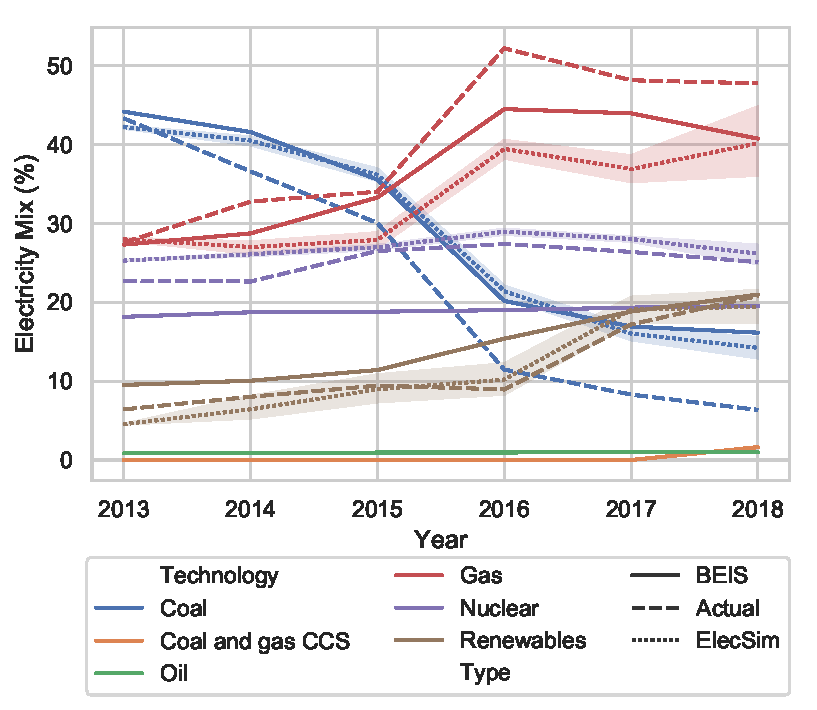
\includegraphics[width=0.7\columnwidth]{Chapter4/figures/e-Energy-2020/results/throughout_years_beis_elecsim_comparison_coal_dropout_leg_below.pdf}
	\caption{Comparison of actual electricity mix vs. ElecSim vs. BEIS projections and taking three coal power plants out of service.}
	\label{elecsim:fig:beis_elecsim_historic_comparison}
\end{figure}

The observed electricity mix changed significantly between 2013 and 2018. A continuous decrease of electricity production from coal throughout this period was observed. 2015 and 2016 saw a marked decrease of coal, which can be explained by the retirement of 3 major coal power plants. The decrease in coal between 2013 and 2016 was largely replaced by an increase in gas. After 2016, renewables play an increasingly large role in the electricity mix and displace gas.

Both ElecSim and BEIS were able to model the fundamental dynamics of this shift from coal to gas as well as the increase in renewables. Both models, however, underestimated the magnitude of the shift from coal to gas. This could be due to unmodelled behaviours such as consumer sentiment towards highly polluting coal plants, a prediction from industry that gas would become more economically attractive in the future or a reaction to The Energy Act 2013 which aimed to close a number of coal power stations over the following two decades \cite{uk_energy_act}.

%Both ElecSim and BEIS performed similarly in projecting the uptake in renewables. Whilst both models were able to accurately project the final renewable electricity mix in 2018, the observed uptake in renewables began to increase in 2015, as opposed to 2016. This could be explained by the increased wind speeds and rainfall observed during 2015 \cite{pa_2013_renewables}.

ElecSim was able to closely model the increase in renewables throughout the period in question, specifically predicting a dramatic increase in 2017. This is in contrast to BEIS who predicted that an increase in renewable energy would begin in 2016. However, both models were able to accurately predict the proportion of renewables in 2018. 

ElecSim was able to better model the observed fluctuation in nuclear power in 2016. BEIS, on the other hand, projected a more consistent nuclear energy output. This small increase in nuclear power is likely due to the decrease in coal during that year. BEIS consistently underestimated the share of nuclear power. 


%ElecSim and BEIS performed similarly with respect to the uptake in renewable energy  


%\subsection{Validation results and comparison}


%Figure \ref{fig:actual_vs_simulated_validation} shows the simulated electricity mix compared to the actual electricity mix between the years of 2013 to 2018 for the best price duration parameter set.


%\begin{figure}
%\centering
%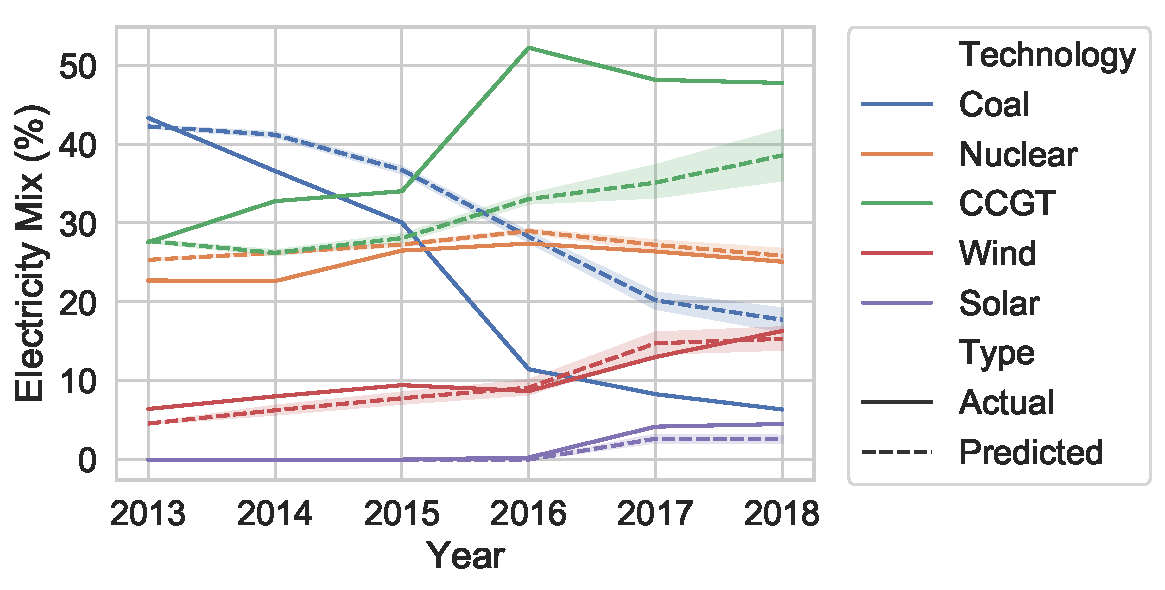
\includegraphics[width=0.49\textwidth]{figures/results/throughout_years.pdf}
%\caption{Electricity mix actual vs. simulated for validation scenario with eight representative days.}
%\label{fig:actual_vs_simulated_validation}
%\end{figure}

%


%Figure \ref{fig:actual_vs_simulated_validation} shows a rapid uptakes in solar and wind from the year of 2016, which closely matches the actual uptake. As well as this, the actual mix displays a rapid transition from coal to CCGT. Whilst ElecSim matches this trend, it is not matched precisely. 
%
%Figure \ref{fig:uk_validated_results_2018} compares the electricity mix in the year 2018 for actual and simulated by ElecSim for the optimal predicted price duration curve. 




%We compare our projections from 2013 to 2018 with the UK Governments (BEIS) projections made in 2013 in Figure \ref{fig:beis_elecsim_historic_comparison} \cite{UKDECC2013}. BEIS were also unable to precisley match the transition from coal to CCGT. However, they were able to model the large transition of coal to CCGT in the year 2016.
%
%However, the BEIS projection overestimates the uptake in renewables in the year 2016, which ElecSim does not.


%\begin{figure}
%\centering
%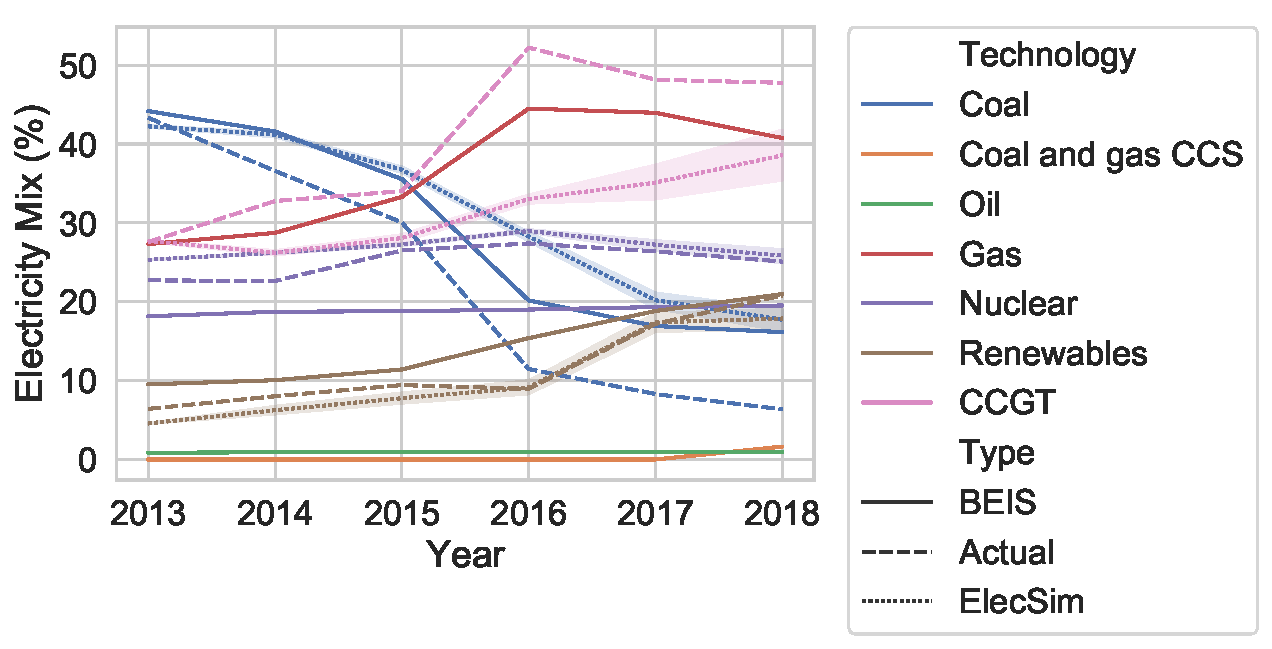
\includegraphics[width=0.49\textwidth]{figures/results/throughout_years_beis_elecsim_comparison.pdf}
%\caption{Comparison of actual electricity mix vs. ElecSim vs. BEIS projections.}
%\label{fig:beis_elecsim_historic_comparison}
%\end{figure}



%\begin{figure}
%\centering
%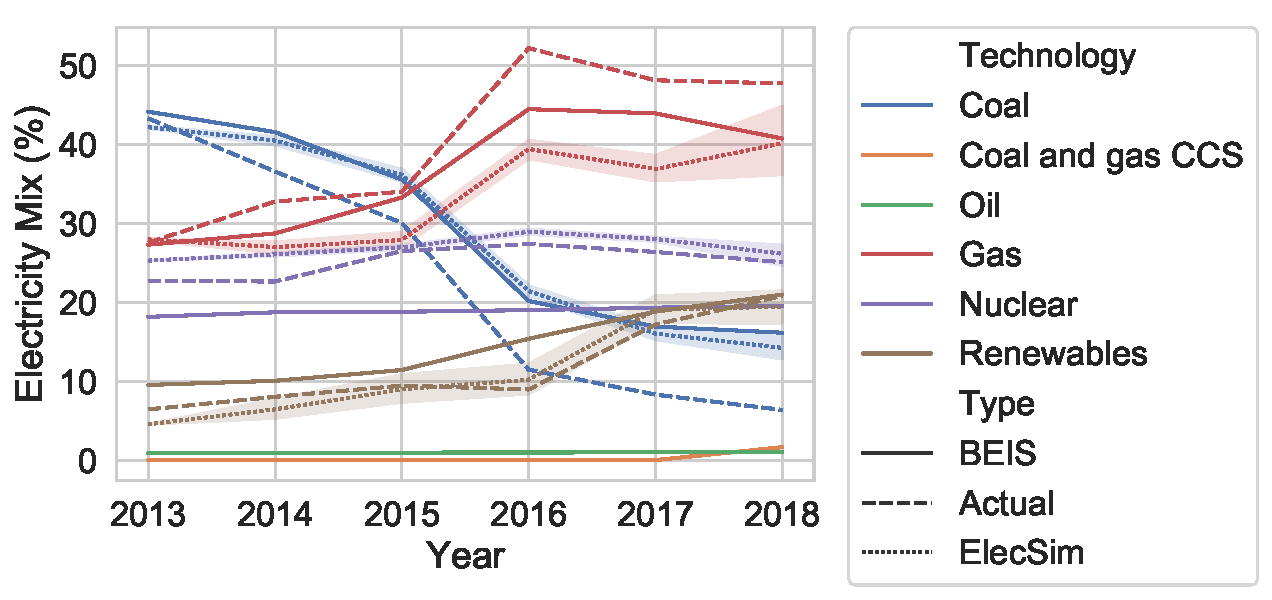
\includegraphics[width=0.49\textwidth]{figures/results/throughout_years_beis_elecsim_comparison_coal_dropout.pdf}
%\caption{Comparison of actual electricity mix vs. ElecSim vs. BEIS projections and taking three coal power plants out of service.}
%\label{fig:beis_elecsim_historic_comparison}
%\end{figure}






We display the error metrics to evaluate our models 5 year projections in Table \ref{table:metrics}. Where MAE is mean absolute squared error, MASE is mean absolute scaled error and RMSE is root mean squared error.

We are able to improve the projections for all generation types when compared to the naive forecasting approach using ElecSim, as shown by the MASE. Where the naive approach is simply predicting the next time-step by using the last known time-step. In this case the last known time-step is the electricity mix percentage for each generation type in 2013. 

\begin{table}[htb]
	\centering
	\csvautobooktabular{Chapter4/table_data/results/error_metrics.csv}
	\caption{Error metrics for time series forecast from 2013 to 2018.}
	\label{table:metrics}
\end{table}

Figure \ref{fig:best_price_curve} displays the optimal predicted price duration curve ($PPDC$) found by the genetic algorithm. This price curve was used by the GenCos to achieve the results shown in Figure \ref{fig:beis_elecsim_historic_comparison}. 


\begin{figure}
	\centering
	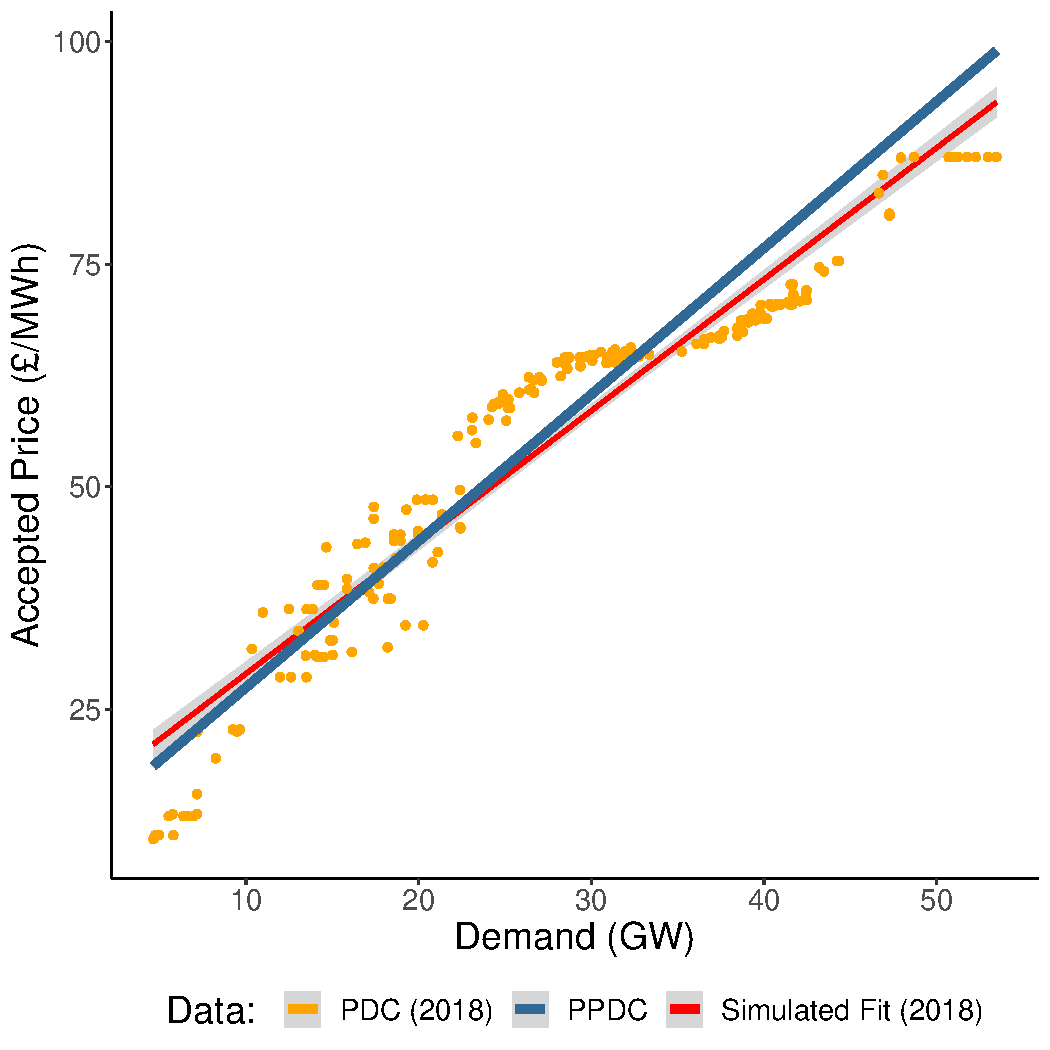
\includegraphics[width=0.65\textwidth]{Chapter4/figures/e-Energy-2020/results/best_run_price_dur_curve.pdf}
	\caption{Predicted price duration curve for investment for most accurate run against simulated run in 2018.}
	\label{fig:best_price_curve}
\end{figure}

The yellow points show the simulated price duration curve for the first year of the simulation (2018). The red line (Simulated Fit (2018)) is a linear regression that approximates the simulated price duration curve (PDC (2018)). The blue line shows the price duration curve predicted ($PPDC$) by the GenCos to be representative of the expected prices over the lifetime of the plant.

%The blue line is the price duration curve simulated in 2018, and the red line is the optimal predicted electricity mix. 

The optimal predicted price duration curve ($PPDC$) closely matches the simulated fit in 2018, shown by Figure \ref{fig:best_price_curve}. However, the $PPDC$ has a slightly higher peak price and lower baseload price. This could be due to the fact that there is a predicted increase in the number of renewables with a low SRMC. However, due to the intermittency of renewables such as solar and wind, higher peak prices are required to generate in times of low wind and solar irradiance at the earth's surface.






To generate Figure \ref{fig:uk_validated_results_2018}, we ran 40 scenarios with the $PPDC$ to observe the final, simulated electricity mix. The error bars are computed based on a Normal distribution 95\% confidence interval.

ElecSim was able to model the increase in renewables and stability of nuclear energy in this time. ElecSim was also able to model the transition from coal to gas, however, underestimated the magnitude of the transition. This was similar to the projections BEIS made in 2013 as previously discussed.

\begin{figure}
	\centering
	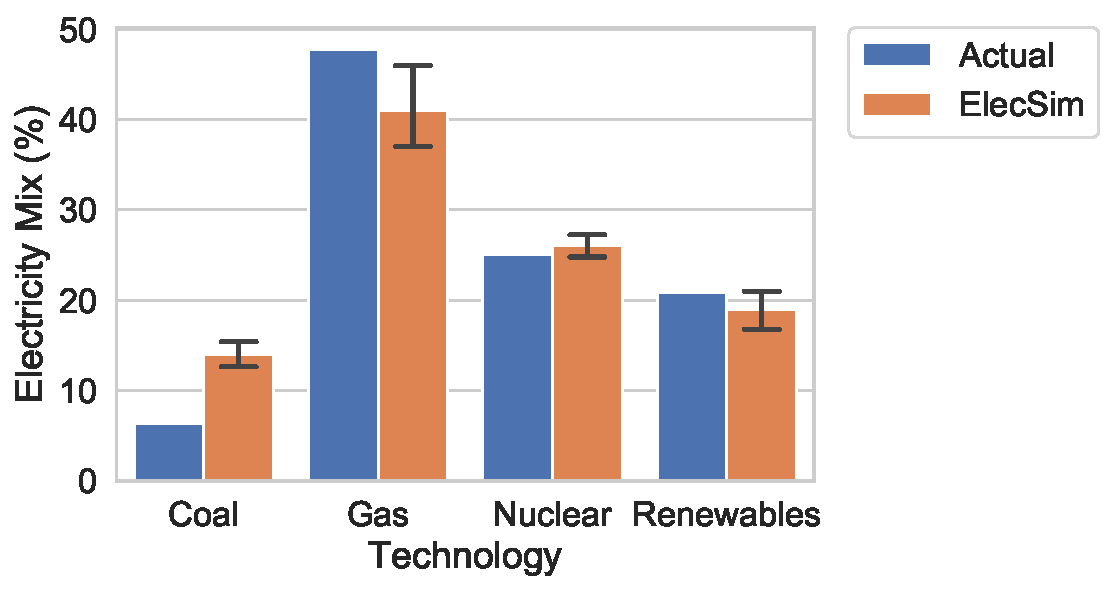
\includegraphics[width=0.65\textwidth]{Chapter4/figures/e-Energy-2020/results/best_run_coal_dropout_95_ci.pdf}
	\caption{Electricity generation mix simulated by ElecSim from 2013 to 2018 compared to observed electricity mix in 2018.}
	\label{fig:uk_validated_results_2018}
\end{figure}

%Figure \ref{fig:single_time_step_results} displays the results using the same scenario details such as fuel and carbon price, electricity generation costs and GenCos. As mentioned in Section \ref{ssec:representative_days}, we see an overestimation in the uptakes of IRES. In this case all electricity sources are replaced by wind which with current storage technologies is not possible.



%\begin{figure}
%\centering
%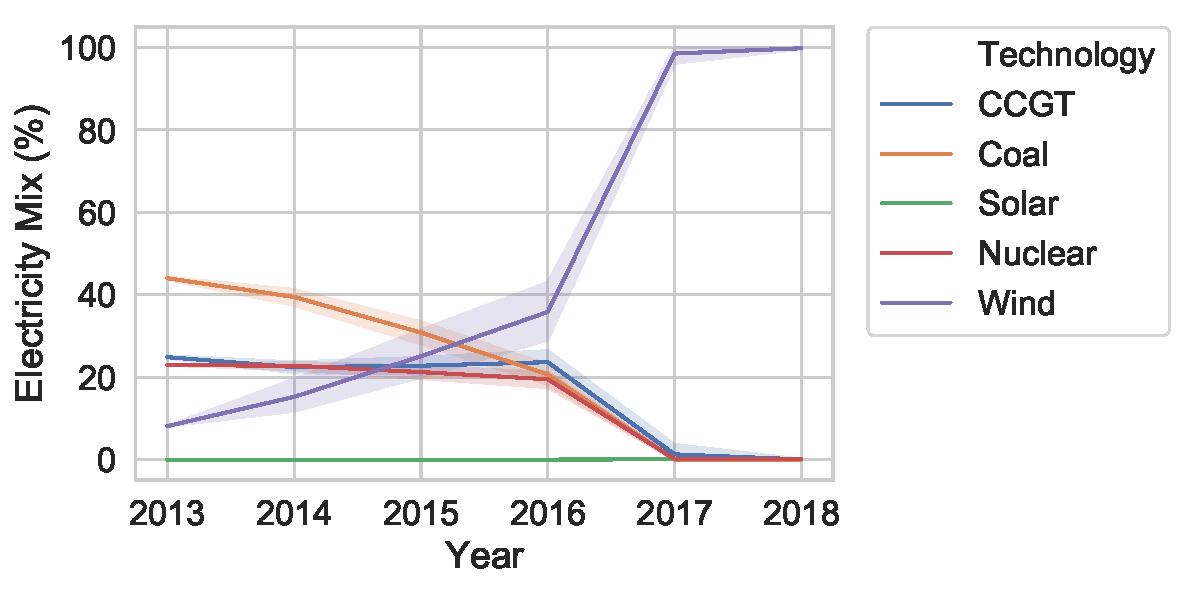
\includegraphics[width=0.49\textwidth]{figures/results/yearly_time_step_scenario.pdf}
%\caption{Electricity mix actual vs. simulated for validation scenario with a single representative day.}
%\label{fig:single_time_step_results}
%\end{figure}



\subsubsection{Long-Term Scenario Analysis}

In this section we discuss the results of the analysis of the BEIS reference scenario explained in Section \ref{sssec:scen-analysis}. Specifically, we created a scenario that mimicked that of BEIS in ElecSim and optimised a number of parameters using a genetic algorithm to match this scenario. Through this we are able to gain confidence in the underlying dynamics of ElecSim to simulate long-term behaviours. Further, this enables us to verify the likelihood of the scenario by analysing whether the parameters required to make such a scenario are realistic.

Figure \ref{fig:forward_scenario_beis_elecsim} displays the electricity mix projected by both ElecSim and BEIS. To generate this image we ran 60 scenarios under the optimal collection of predicted price duration curves, nuclear subsidy and uncertainty in predicted price duration curves. 

The optimal parameters were chosen by choosing the parameter set with the lowest mean error per electricity generation type and per year throughout the simulation, as shown by Equation \ref{eq:long-term-reward}.


Figure \ref{fig:forward_scenario_best_pdcs} displays the optimal predicted price duration curves ($PPDC$s) per year of the simulation, shown in blue. These are compared to the price duration curve simulated in 2018, as per Figure \ref{fig:best_price_curve}. The optimal nuclear subsidy, $S_n$, was found to be ${\sim}$\textsterling $120$, the optimal $\sigma_m$ and $\sigma_c$ were found to be $0$ and ${\sim}0.0006$ respectively.

The BEIS scenario demonstrates a progressive increase in nuclear energy from 2025 to 2035, a consistent decrease in electricity produced by natural gas, an increase in renewables and decrease to almost 0\% by 2026 of coal.

ElecSim is largely able to mimic the scenario by BEIS. A large increase in renewables is projected, followed by a decrease in natural gas. 

A significant difference, however, is the step-change in nuclear power in 2033. This led to an almost equal reduction in natural gas during the same year. In contrast, BEIS project a continuously increasing share of nuclear. 

We argue that the ElecSim projection of nuclear power is more realistic than that of BEIS due to the instantaneous nature of large nuclear power plants coming on-line.

Figure \ref{fig:forward_scenario_best_pdcs} exhibits the price curves required to generate the scenario show in Figure \ref{fig:forward_scenario_beis_elecsim}. The majority of the price curves are similar to the simulated price duration curve of 2018 (Simulated Fit (2018)). However, there are some price curves which are significantly higher and significantly lower than the predicted price curve of 2018. These cycles in predicted price duration curves may be explained by investment cycles typically exhibited in electricity markets \cite{Gross2007}. 

In this context, investment cycles reflect a boom and bust cycle over long timescales. When electricity supply becomes tight relative to demand, prices rise to create an incentive to invest in new capacity. Price behaviour in competitive markets can lead to periods of several years of low prices (close to short-run marginal cost) \cite{white2005concentrated}. 

As plants retire or demand increases, the market becomes tighter until average prices increase to a level above the threshold for investment in new power generators. At this point investors may race to bring new plants on-line to make the most out of the higher prices. Once adequate investments have been made, the market returns to a period of low prices and low investment until the next price spike \cite{Gross2007}. 


The nuclear subsidy, $S_n$, of ${\sim}$\textsterling $120$ in 2018 prices is high compared to similar subsidies, but this may reflect the difficulty of nuclear competing with renewable technology with a short-run marginal cost that tends to \textsterling $0$.

The low values of $\sigma_m$ and $\sigma_c$ demonstrates that the expectation of prices does not necessarily have to differ significantly between GenCos. This may be due to the fact that GenCos have access to the same market information.


\begin{figure}
	\centering
	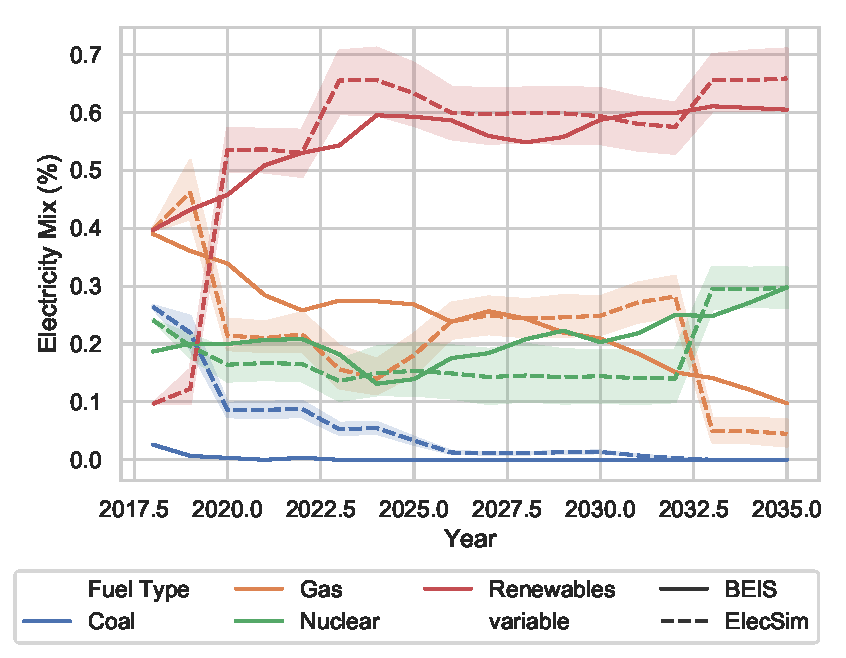
\includegraphics[width=0.60\textwidth]{Chapter4/figures/e-Energy-2020/results/scenario_analysis/best_forward_scenario_below_legend.pdf}
	\caption{Comparison of ElecSim and BEIS' reference scenario from 2018 to 2035.}
	\label{fig:forward_scenario_beis_elecsim}
\end{figure}



\begin{figure}
	\centering
	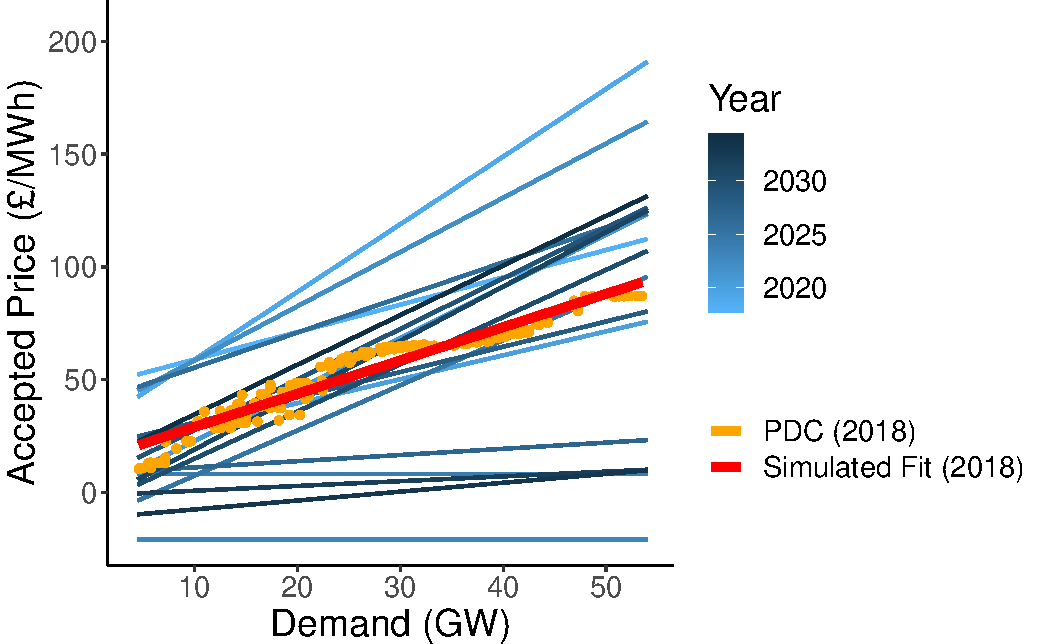
\includegraphics[width=0.6\textwidth, keepaspectratio]{Chapter4/figures/e-Energy-2020/results/scenario_analysis/optimal_pdc_prices.pdf}
	\caption{Comparison between optimal price duration curves and simulated price duration curve in 2018.}
	\label{fig:forward_scenario_best_pdcs}
\end{figure}


%\begin{figure}
%\centering
%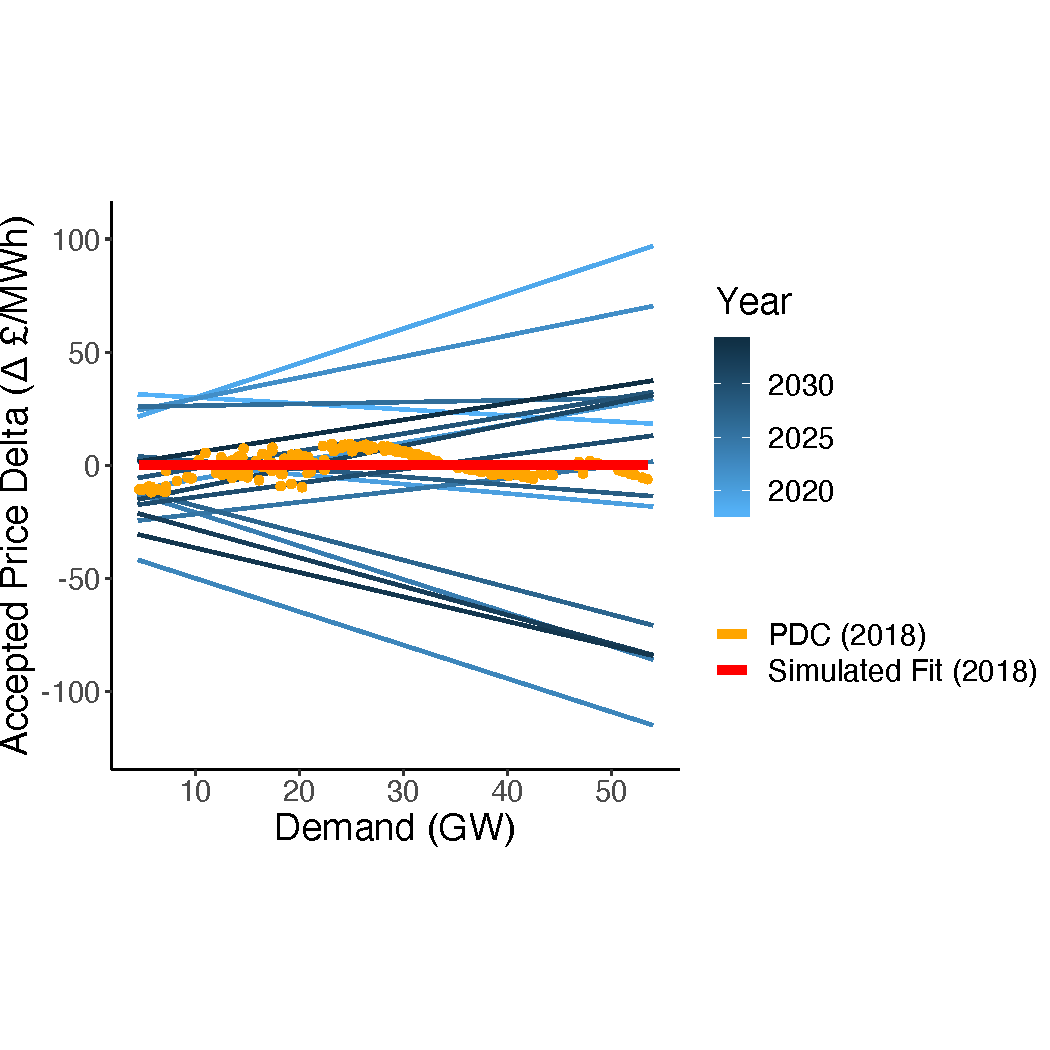
\includegraphics[width=0.49\textwidth, height=0.49\textwidth, keepaspectratio]{figures/results/scenario_analysis/optimal_pdc_prices_differences_delta.pdf}
%\caption{Comparison between optimal price duration curves and simulated price duration curve in 2018.}
%\label{fig:forward_scenario_best_pdcs}
%\end{figure}




\clearpage
\section{Scenario Testing}
\label{elecsim:sec:scenarios}

In this Section we display scenario runs of ElecSim using 20 time-steps per year and using representative days

\subsection{Scenarios for 20 time-steps}

In this section we present example scenario runs using ElecSim with 20 time-steps. We vary the carbon tax and grow or reduce total electricity demand. This enables us to observe the effects of carbon tax on investment. In this paper, we have presented scenarios where electricity demand decreases 1\% per year, due to the recent trend in the UK.

%ElecSim was built using python, this enabled us to lower barriers to entry and allow for users to integrate state-of-the-art machine learning and statistical packages in future work. We used project mesa as an open source agent based modelling framework for its ease of use \cite{Masad2015}.

% {\color{blue}
% We assume that carbon tax is set by the government, and not subject to market forces such as the EU Emissions Trading Scheme \cite{Council2016}.

% We run 16 different scenarios 8 times each, with demand increasing and decreasing by 1\% per year and  varying carbon prices. In this section we explore a decreasing demand of 1\% a year. We chose this due to the increasing efficiency of homes, industry and technology, and due to the recent trend in the UK. Demand, however, did not display a large effect on the optimum carbon price. We select a burn-in period of 6 years, due to the fact that the majority of power plants take 6 years to go from investment to operation.

% Table \ref{table:scenario_statistics}, in the appendix, displays the summary statistics of each run.

% It can be seen from Figure \ref{fig:demand99carbon10} that a carbon tax of \textsterling10 per year does little to influence investment in low-carbon, renewable technology. With traditional, fossil fuel based generation, providing the majority of supply in each year. However, there is an increase in renewable technology over the years, starting from mean 15.85\% market share in the year range 2019-2029, to 24.38\% in the year range 2039-2050. A similar increase of renewable energy with a carbon tax of \textsterling0 can be seen, albeit at a lower mean by the year range 2039-2050 (22.29\%).
% }

For the first scenario run displayed, we have approximated the predictions by the UK Government, where carbon tax increases linearly from \textsterling18 to \textsterling200 by 2050 \cite{Department2016}. Figure \ref{fig:demand99carbon18} demonstrates a significant increase in gas turbines in the first few years, followed by a decrease, with onshore wind increasing.

Figure \ref{fig:demand99carbon40} displays a run with a \textsterling40 carbon tax. This run demonstrates a higher share of onshore wind than in the previous scenario. 

We experimented with the following levels of carbon tax: \textsterling10 (\$13), \textsterling20 (\$26) and \textsterling70 (\$90) with demand decreasing 1\% per year. This was chosen due to the increasing efficiency of homes, industry and technology, and due to the recent trend in the UK. We run each scenario 8 times to capture the stochastic nature of the process. Via the observation of the emergent investment behaviour until 2050, an understanding of how real life investors may behave emerges.


Figure \ref{fig:demand99carbon10} shows that with a carbon tax of \textsterling10, whilst renewable technology does grow, gas power plants provide the majority of supply in each year. However, at a level of \textsterling20 the increase in wind turbines is enough to match gas turbines. A carbon tax of \textsterling70, however, shows a near 100\% uptake of wind turbines.

It is infeasible for the power supply to be provided solely by wind turbines today. This overestimation, however, is due to the low time granularity of the model \cite{Collins2017}. This scenario therefore assumes perfect storage capabilities.



These runs demonstrate that a consistent, but relatively low carbon tax can have a larger impact in the uptake of renewable energy than increasing carbon tax over a long time frame. We hypothesise that an early carbon tax affects the long-term dynamics of the market for many years. We, therefore, suggest early action on carbon tax to transition to a low-carbon energy supply


%The UK Government BEIS have predicted a carbon tax increasing from \textsterling18 to \textsterling200 by 2050, with carbon price increasingly linearly from 2030 to 2050 \cite{Department2016}. We have approximated these assumptions and modelled the results, shown by Figure \ref{fig:demand99carbon18}. The results show only a slight decrease in low-carbon supply over the \textsterling40 carbon tax energy mix. This demonstrates the importance of long-term modelling, and understanding the long-term impacts that can result. It is hypothesised that a lower carbon tax early on changes the market dynamics for years to come, due to certain price structures.
%
%Figure \ref{fig:demand99carbon40} shows that a carbon tax of \textsterling40 is sufficient in moving towards a low-carbon economy, with backup fossil fuel generators.

% {\color{blue}However, by referring to Figure \ref{fig:demand99carbon70} it can be seen that to have 100\% renewable, a carbon price of \textsterling70 is required.

% These results show the importance of making difficult decisions as soon as possible to have the biggest effect on the energy mix for years to come.}

% \begin{figure}
% \begin{center}
% 		\includegraphics[width=0.5\textwidth]{figures/scenarios/demand099-carbon70-datetime.png}
% 		\caption{{\color{blue}Demand decreasing by 1\% per year with a carbon tax of \textsterling70.}}
% 		\label{fig:demand99carbon70}
% 	\end{center}
% \end{figure}



% \begin{figure*}[h]
% 	\centering
% 	\begin{subfigure}[b]{0.475\textwidth}
% 		\centering
% 		\includegraphics[width=\textwidth]{figures/scenarios/demand099-carbon10-datetime.png}
% 		\caption[Network2]%
% 		{{{\color{blue}{\small \textsterling10 carbon tax.}}}}
% 		\label{fig:demand99carbon10}
% 	\end{subfigure}
% 	\hfill
% 	\begin{subfigure}[b]{0.475\textwidth}  
% 		\centering 
% 		\includegraphics[width=\textwidth]{figures/scenarios/demand099-carbon20-datetime.png}
% 		\caption[]%
% 		{{{\color{blue}\textsterling20 carbon tax.}}}
% 		\label{fig:demand99carbon20}
% 	\end{subfigure}
% 	\vskip\baselineskip

%
%	\begin{subfigure}[b]{0.475\textwidth}   
%		\centering 
%		\includegraphics[width=\textwidth]{figures/scenarios/demand099-carbon18-datetime.png}
%		\caption[]%
%		{{\textsterling26 to \textsterling150 linearly increasing carbon tax.}}    
%		\label{fig:demand99carbon18}
%	\end{subfigure}
%	\quad
%	\begin{subfigure}[b]{0.475\textwidth}   
%		\centering 
%		\includegraphics[width=\textwidth]{figures/scenarios/demand099-carbon40-datetime.png}
%		\caption[]%
%		{{\textsterling40 carbon tax.}}    
%		\label{fig:demand99carbon40}
%	\end{subfigure}
%	\caption[ Scenarios up to the year 2050 with varying carbon taxes and decreasing demand ]
%	{\small Scenarios up to the year 2050, with varying carbon taxes and electricity demand decreasing 1\% a year.} 
%	\label{fig:mean and std of nets}
%\end{figure*}
%\FloatBarrier

%\begin{figure}[b]{0.475\columnwidth}   
%	\centering 
%	\includegraphics{figures/scenarios/demand099-carbon18-datetime.png}
%	\caption[]%
%	{{\textsterling26 to \textsterling150 linearly increasing carbon tax.}}    
%	\label{fig:demand99carbon18}
%\end{figure}
%
%\begin{figure}[b]{0.475\columnwidth}   
%	\centering 
%	\includegraphics{figures/scenarios/demand099-carbon40-datetime.png}
%	\caption[]%
%	{{\textsterling40 carbon tax.}}    
%	\label{fig:demand99carbon40}
%\end{figure}

\begin{figure}
	\centering
	\begin{subfigure}{.7\linewidth}
		\includegraphics[width=0.6\linewidth]{Chapter4/figures/scenarios/demand099-carbon18-datetime.png}
		\caption{\textsterling26 to \textsterling150 linearly increasing carbon tax.}
		\label{fig:demand99carbon18}
	\end{subfigure}
	\begin{subfigure}{.7\linewidth}
		\includegraphics[width=0.6\linewidth]{Chapter4/figures/scenarios/demand099-carbon40-datetime.png}
		\caption{{\textsterling40 carbon tax}}
		\label{fig:demand99carbon40}
	\end{subfigure}
	\caption{Scenarios with varying carbon taxes and decreasing demand (-1\%/year)}
\end{figure}






%\begin{figure}[h]
%	\begin{center}
%		\includegraphics[width=0.5\textwidth]{figures/scenarios/demand099-carbon10-datetime.png}
%		\caption{Demand decreasing by 1\% per year and a carbon tax of \textsterling10}
%		\label{fig:demand99carbon10}
%	\end{center}
%\end{figure}
%
%\begin{figure}[h]
%	\begin{center}
%		\includegraphics[width=0.5\textwidth]{figures/scenarios/demand099-carbon20-datetime.png}
%		\caption{Demand decreasing by 1\% per year and a carbon tax of \textsterling20}
%		\label{fig:demand99carbon10}
%	\end{center}
%\end{figure}
%
%
%
%\begin{figure}[h]
%	\begin{center}
%		\includegraphics[width=0.5\textwidth]{figures/scenarios/demand099-carbon18-datetime.png}
%		\caption{Demand decreasing by 1\% per year and a carbon tax of \textsterling20}
%		\label{fig:demand99carbon10}
%	\end{center}
%\end{figure}
%
%
%
%\begin{figure}[h]
%	\begin{center}
%		\includegraphics[width=0.5\textwidth]{figures/scenarios/demand099-carbon40-datetime.png}
%		\caption{Demand decreasing by 1\% per year and a carbon tax of \textsterling20}
%		\label{fig:demand99carbon10}
%	\end{center}
%\end{figure}
%\begin{figure}
%	\centering
%	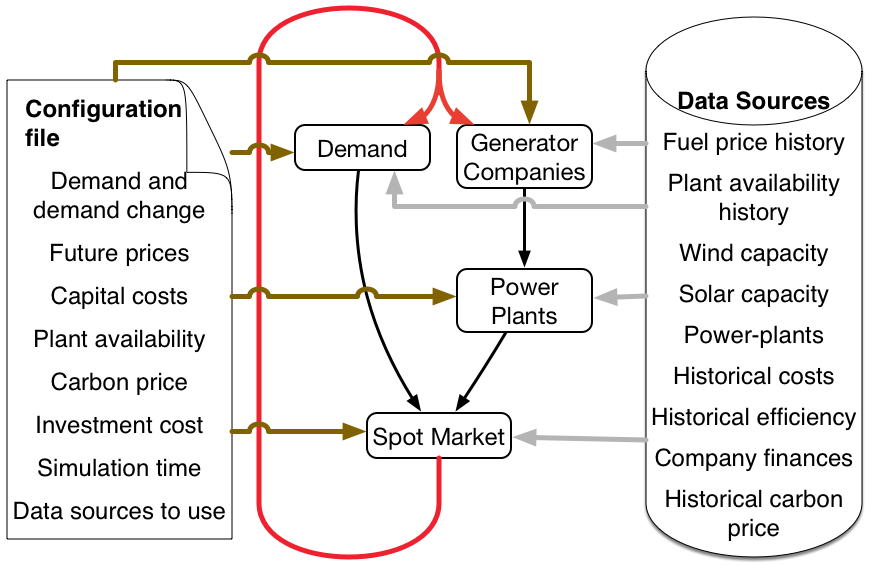
\includegraphics[width=0.85\linewidth]{Chapter4/figures/System_overview_large}
%	\caption{System overview of agent-based market model.}
%	\label{fig:systemoverview}
%	\vskip -6mm
%\end{figure}


\begin{figure}[h]
	\centering
	\begin{subfigure}[b]{0.6\textwidth}
		\centering
		\includegraphics[width=\textwidth]{Chapter4/figures/scenarios/demand099-carbon10-datetime.png}
		\caption[Network2]%
		{\small \textsterling10 carbon tax.}
		\label{fig:demand99carbon10}
	\end{subfigure}
	\hfill
	\begin{subfigure}[b]{0.6\textwidth}  
		\centering 
		\includegraphics[width=\textwidth]{Chapter4/figures/scenarios/demand099-carbon20-datetime.png}
		\caption[]%
		{\textsterling20 carbon tax.}
		\label{fig:demand99carbon20}
	\end{subfigure}
	\begin{subfigure}[b]{0.6\textwidth}
		\centering
		\includegraphics[width=\textwidth]{Chapter4/figures/scenarios/demand099-carbon70-datetime.png}
		\caption[Network2]%
		{\small \textsterling70 carbon tax.}
		\label{fig:demand99carbon70}
	\end{subfigure}
	\caption{Scenarios from 2020 to 2050 with varying carbon tax.}
\end{figure}









\subsection{Conclusion}


Agent-based models provide a method of simulating investor behaviour in an electricity market. We observed that an increase in carbon tax had a significant impact on investment. These findings enable policy makers to better understand the impact that their decisions may have. For a high uptake of renewable energy technology, rapid results can be seen after 10 years with a carbon tax of \textsterling70 (\$90).




\subsection{Scenarios for representative days}

In this section we discuss various scenarios under the model which uses representative days as time-steps. This work builds upon the work in Section \ref{architecture:sec:validation}; we used the same predicted price duration curves as modelled on BEIS' scenario. We selected an optimal carbon tax level which would reduce both electricity price and carbon emissions, as shown later in Chapter \ref{chapter:carbon}. The optimal carbon tax strategy found in Chapter \ref{chapter:carbon} is shown by Figure \ref{elecsim:fig:optimal_carbon_tax_strategy}. Each of the scenarios were run 10 times to display any variability in the results. We chose 10 runs to limit both computation time and cost.



\begin{figure}
	\centering
	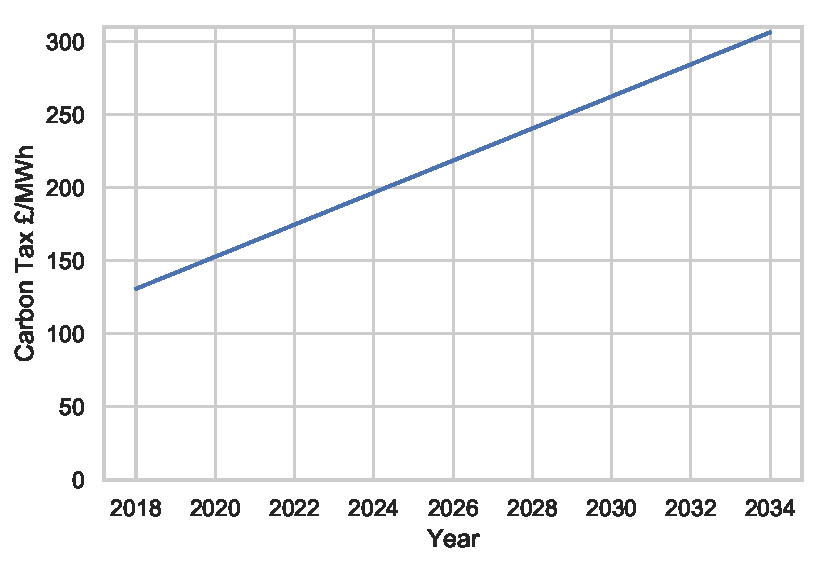
\includegraphics[width=0.7\textwidth, keepaspectratio]{Chapter4/figures/scenarios/representative-day-scenarios/optimal_carbon_strategy.pdf}
	\caption{Optimal carbon tax strategy to reduce both electricity cost and carbon emissions.}
	\label{elecsim:fig:optimal_carbon_tax_strategy}
\end{figure}

Figures \ref{elecsim:fig:increasing_demand} and \ref{elecsim:fig:decreasing_demand} show the electricity mixes of various demand scenarios. Figure \ref{elecsim:fig:increasing_demand} displays the scenarios in which demand either stays flat, or decreases by 1\% and 2\%. For these scenarios it can be seen that solar is the dominant electricity supply, supplying ${\sim}$50\%, with nuclear power in second supplying between 20\% and 30\%. With a decreasing demand scenario of 1\% per year, as shown by Figure \ref{fig:demand099}, nuclear provides a higher proportion by the year 2034, of ${\sim}$30\%, however before the year 2033, provides a similar proportion to the other scenarios as shown by Figures \ref{fig:demand10} and \ref{fig:demand098}.

For the scenarios shown in Figure \ref{elecsim:fig:increasing_demand}, CCGT, coal and onshore provide around ${\sim}$10\% each by 2034.  Coal and CCGT, however, progress towards 0\% whereas onshore wind increases. This is to be expected due to the high carbon price, as shown by Figure \ref{elecsim:fig:optimal_carbon_tax_strategy}. Offshore does not exhibit a high amount of investment. We believe this is the case as offshore wind is more expensive than onshore wind, and in our scenario subsidies other than for nuclear are not modelled.

\begin{figure}
	\centering
	\begin{subfigure}{0.6\textwidth}
		\centering
		
\includegraphics[width=\textwidth]{Chapter4/figures/scenarios/representative-day-scenarios/10_demand_mix.pdf}
		\caption{Demand does not increase or decrease.}
		\label{fig:demand10}
	\end{subfigure}
	\hfill
	\begin{subfigure}{0.6\textwidth}  
		\centering 
		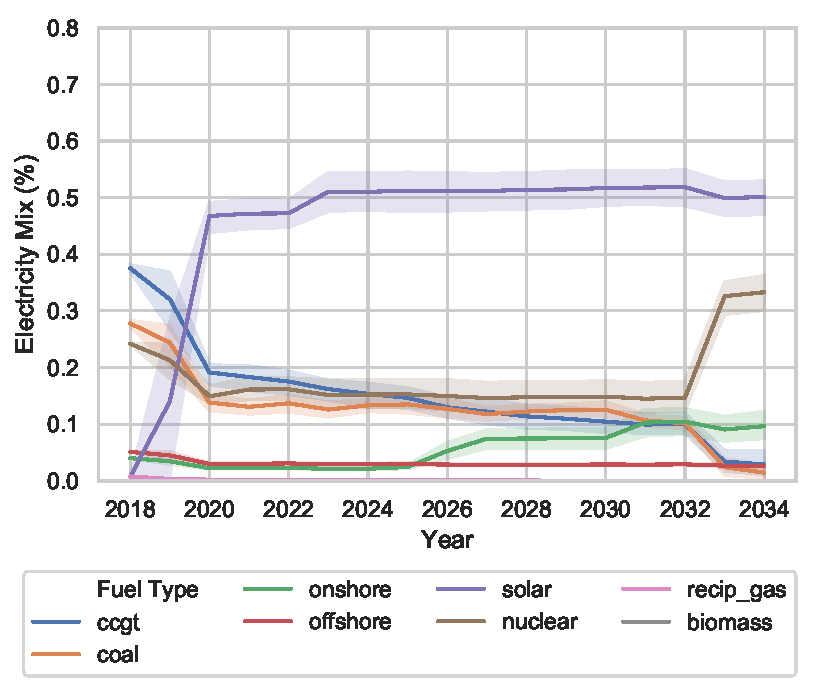
\includegraphics[width=\textwidth]{Chapter4/figures/scenarios/representative-day-scenarios/099_demand_mix.pdf}
		\caption{Demand reduces by 1\% per year.}
		\label{fig:demand099}
	\end{subfigure}
	\begin{subfigure}{0.6\textwidth}
		\centering
		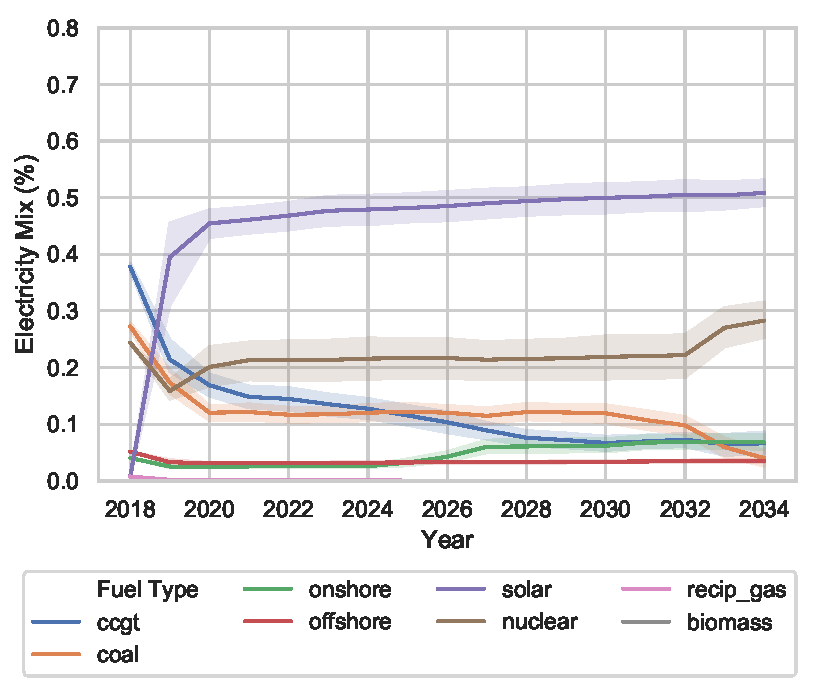
\includegraphics[width=\textwidth]{Chapter4/figures/scenarios/representative-day-scenarios/098_demand_mix.pdf}
		\caption{\small Demand reduces by 2\% per year}
		\label{fig:demand098}
	\end{subfigure}
	\caption{Scenarios from 2018 to 2035 with varying demand.}
	\label{elecsim:fig:increasing_demand}
\end{figure}


Figure \ref{elecsim:fig:decreasing_demand} shows scenarios where demand increases per year. Whilst electricity mix distribution is similar to the scenarios shown in Figure \ref{elecsim:fig:increasing_demand}, solar plays a significantly increased role than nuclear. This may be down to the large expense of nuclear, and the long time of deployment of this type of technology. Solar power, on the other hand, is able to be installed much more quickly to maintain the high demand. This is especially true for the scenarios shown in Figures \ref{fig:demand102} and \ref{fig:demand1025} where demand rises by 2\% and 2.5\% per year respectively. 



\begin{figure}
	\centering
	\begin{subfigure}{0.6\textwidth}
		\centering
		
\includegraphics[width=\textwidth]{Chapter4/figures/scenarios/representative-day-scenarios/101_demand_mix.pdf}
		\caption{\small Demand increases by 1\% per year.}
		\label{fig:demand101}
	\end{subfigure}
	\hfill
	\begin{subfigure}{0.6\textwidth}  
		\centering 
		
\includegraphics[width=\textwidth]{Chapter4/figures/scenarios/representative-day-scenarios/102_demand_mix.pdf}
		\caption{\small Demand increases by 2\% per year.}
		\label{fig:demand102}
	\end{subfigure}
	\begin{subfigure}{0.6\textwidth}
		\centering
		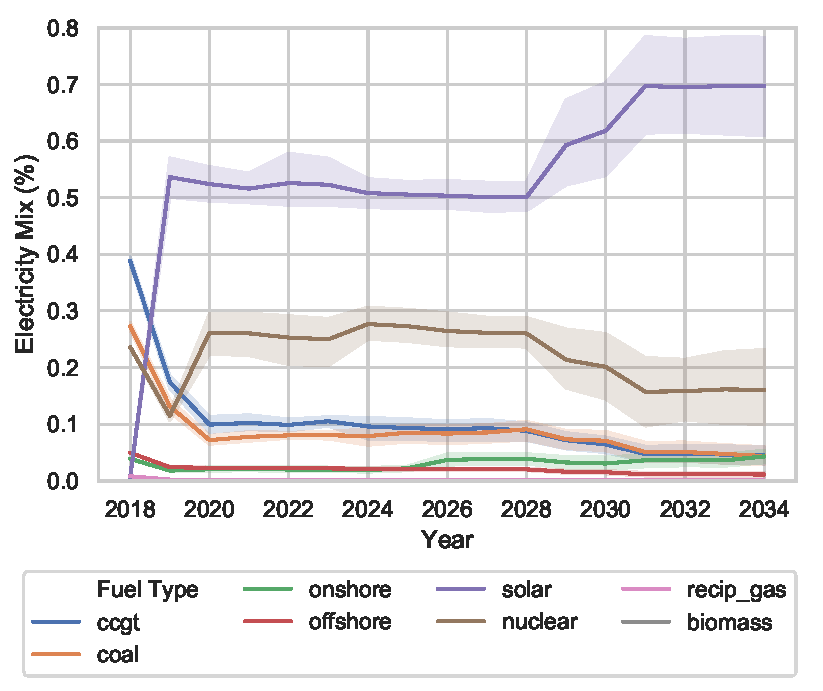
\includegraphics[width=\textwidth]{Chapter4/figures/scenarios/representative-day-scenarios/1025_demand_mix.pdf}
		\caption{\small Demand increases by 2.5\% per year}
		\label{fig:demand1025}
	\end{subfigure}
	\caption{Scenarios from 2018 to 2035 with varying demand.}
	\label{elecsim:fig:decreasing_demand}
\end{figure}























\subsection{Performance}


\begin{figure}
	\centering
	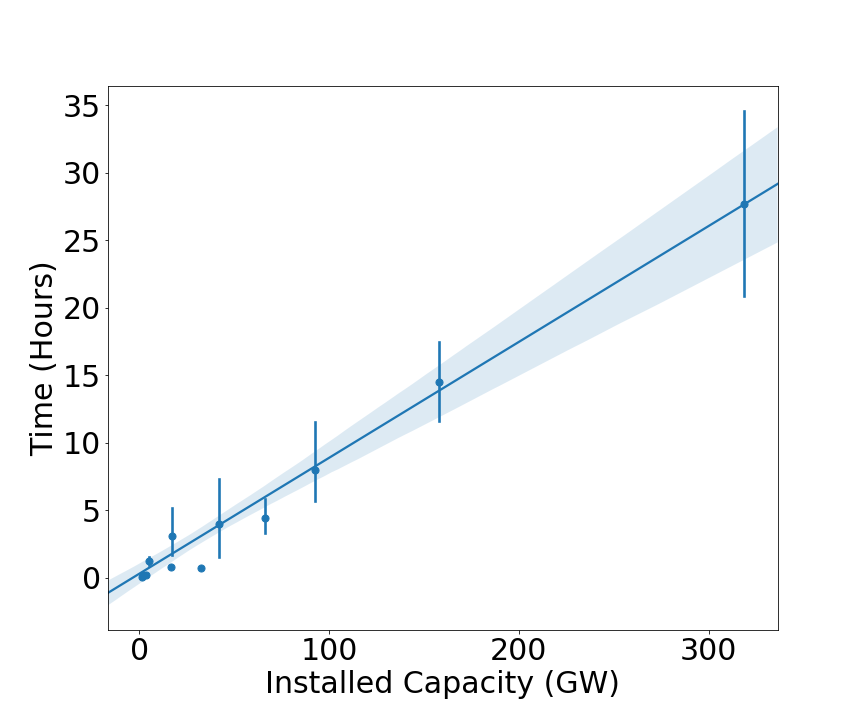
\includegraphics[width=0.6\linewidth]{Chapter4/figures/timing_plot.png}
	\caption{Run times of different sized countries.}
	\label{fig:timingplot}
	\vskip -0.5cm
\end{figure}


Figure \ref{fig:timingplot} shows the running time for ElecSim with varying installed capacity. We varied demand between 2GW and 320GW to see the effect of different sized countries on running time. The makeup of the electricity mix was achieve through stratified sampling of the UK electricity mix. The results show a linear time complexity. 


%\begin{itemize}
%	\item Validation of model 
%	\begin{itemize}
%		\item Compare price duration curve
%		\item Compare power plant costs and NPV calculations
%		\item Look number of steps ahead to compare electricity mix and compare to actual (cross-validation)
%	\end{itemize} 
%	\item Performance metrics - Comparison with EMLab, PowerACE (15 minute run time)
%	\begin{itemize}
%		\item Memory, disk size, runtime
%		\item Increase in time complexity with additional data.
%	\end{itemize}
%\end{itemize}



\clearpage
\section{Sensitivity Analysis}

In this section we investigate a sensitivity analysis of ElecSim, where we vary the weighted average cost of capital and the down payment required for investment. We used the reference scenario discussed in Section \ref{elecsim:sec:scenarios}, with the optimal carbon tax to reduce both emissions and electricity price.

We ran ten iterations per weighted average cost of capital and down payment element. We did this due to the monte-carlo nature of the simulation. We chose ten runs to give us sufficient variance in results, but reduce compute power, to reduce both time and cost of calculation.

\subsection{Results}

Figure \ref{elecsim:fig:wacc_sensitivity} displays the results of the sensitivity analysis for the \Gls{WACC} for non-nuclear power generators. For this, we trialled nine different \acrfull{wacc} values, where a value of 5.9\% is the reference case \cite{KincheloeStephenC1990TWAC}. 

It can be seen that the \acrshort{wacc} has an effect on the total investment in solar, nuclear and CCGT. With a \acrshort{wacc} equal to or greater than 7.4\%, nuclear increases significantly, whilst solar decreases. Nuclear has a \acrshort{wacc} of 10\%, therefore 7.4\% may be the point where nuclear becomes more competitive than solar in an environment where a low-carbon electricity supply is elicited from an optimal carbon tax.

Offshore and coal do not change significantly over different levels of \acrshort{wacc}. This may be due to the fact that CCGT and onshore are more competitive than coal and offshore respectively, without external subsidies. 

Onshore seems to play a larger role at the lowest \acrshort{wacc}, 3.9\%. This may be due to onshore wind's high competitiveness when compared to nuclear.



\begin{figure}
	\centering
	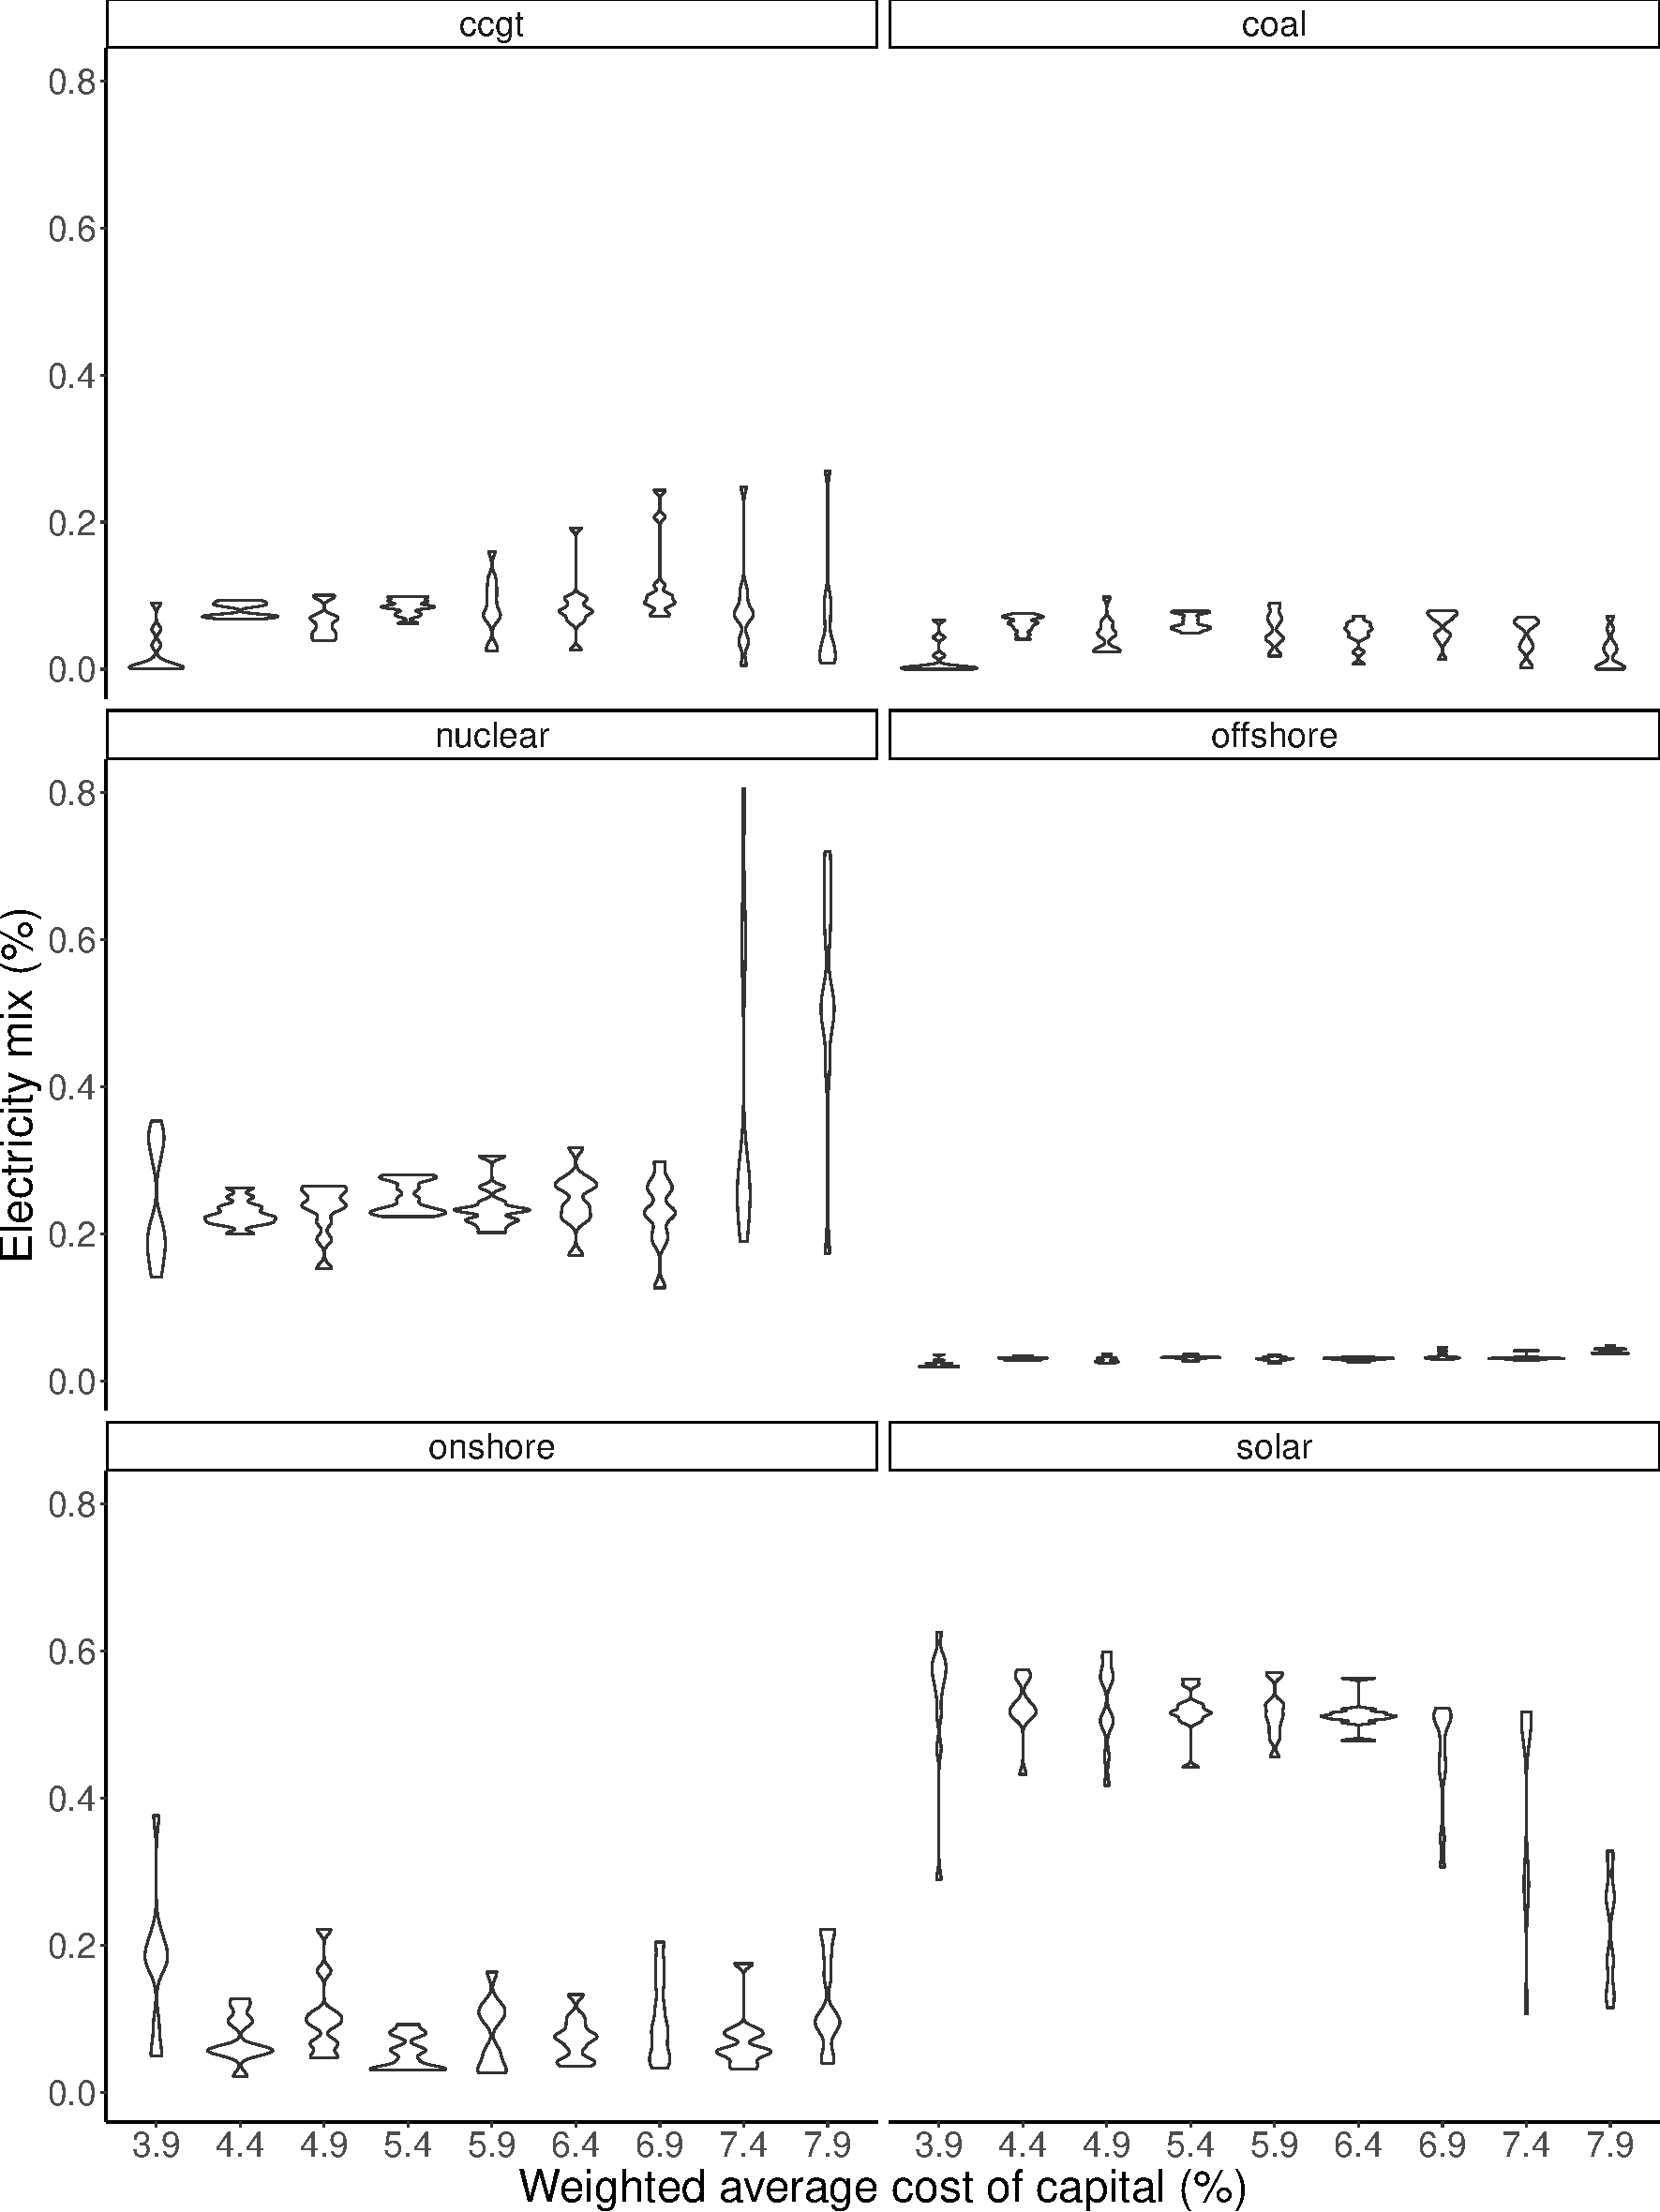
\includegraphics[width=0.9\linewidth]{Chapter4/figures/sensitvity_analysis/wacc_sensitivity_analysis.pdf}
	\caption{Sensitivity analysis where \acrfull{wacc} was varied. Results compare electricity mix in 2035.}
	\label{elecsim:fig:wacc_sensitivity}
\end{figure}

Figure \ref{elecsim:fig:wacc_carbon_sensitivity} displays the relative carbon emissions in 2035. With a low \acrshort{wacc} of 3.9\%, the relative carbon emissions falls, on average, to zero. This seems to be due to the high levels of solar, onshore and nuclear.  

As \acrshort{wacc} increases, so does carbon emissions, until there is a \acrshort{wacc} of 0.5, where it reduces slightly. This is seemingly due to the higher levels of CCGT and coal, which is able to displace solar. However, it must be noted, that in this scenario with the optimal carbon tax, the relative carbon emissions remains low. 


\begin{figure}
	\centering
	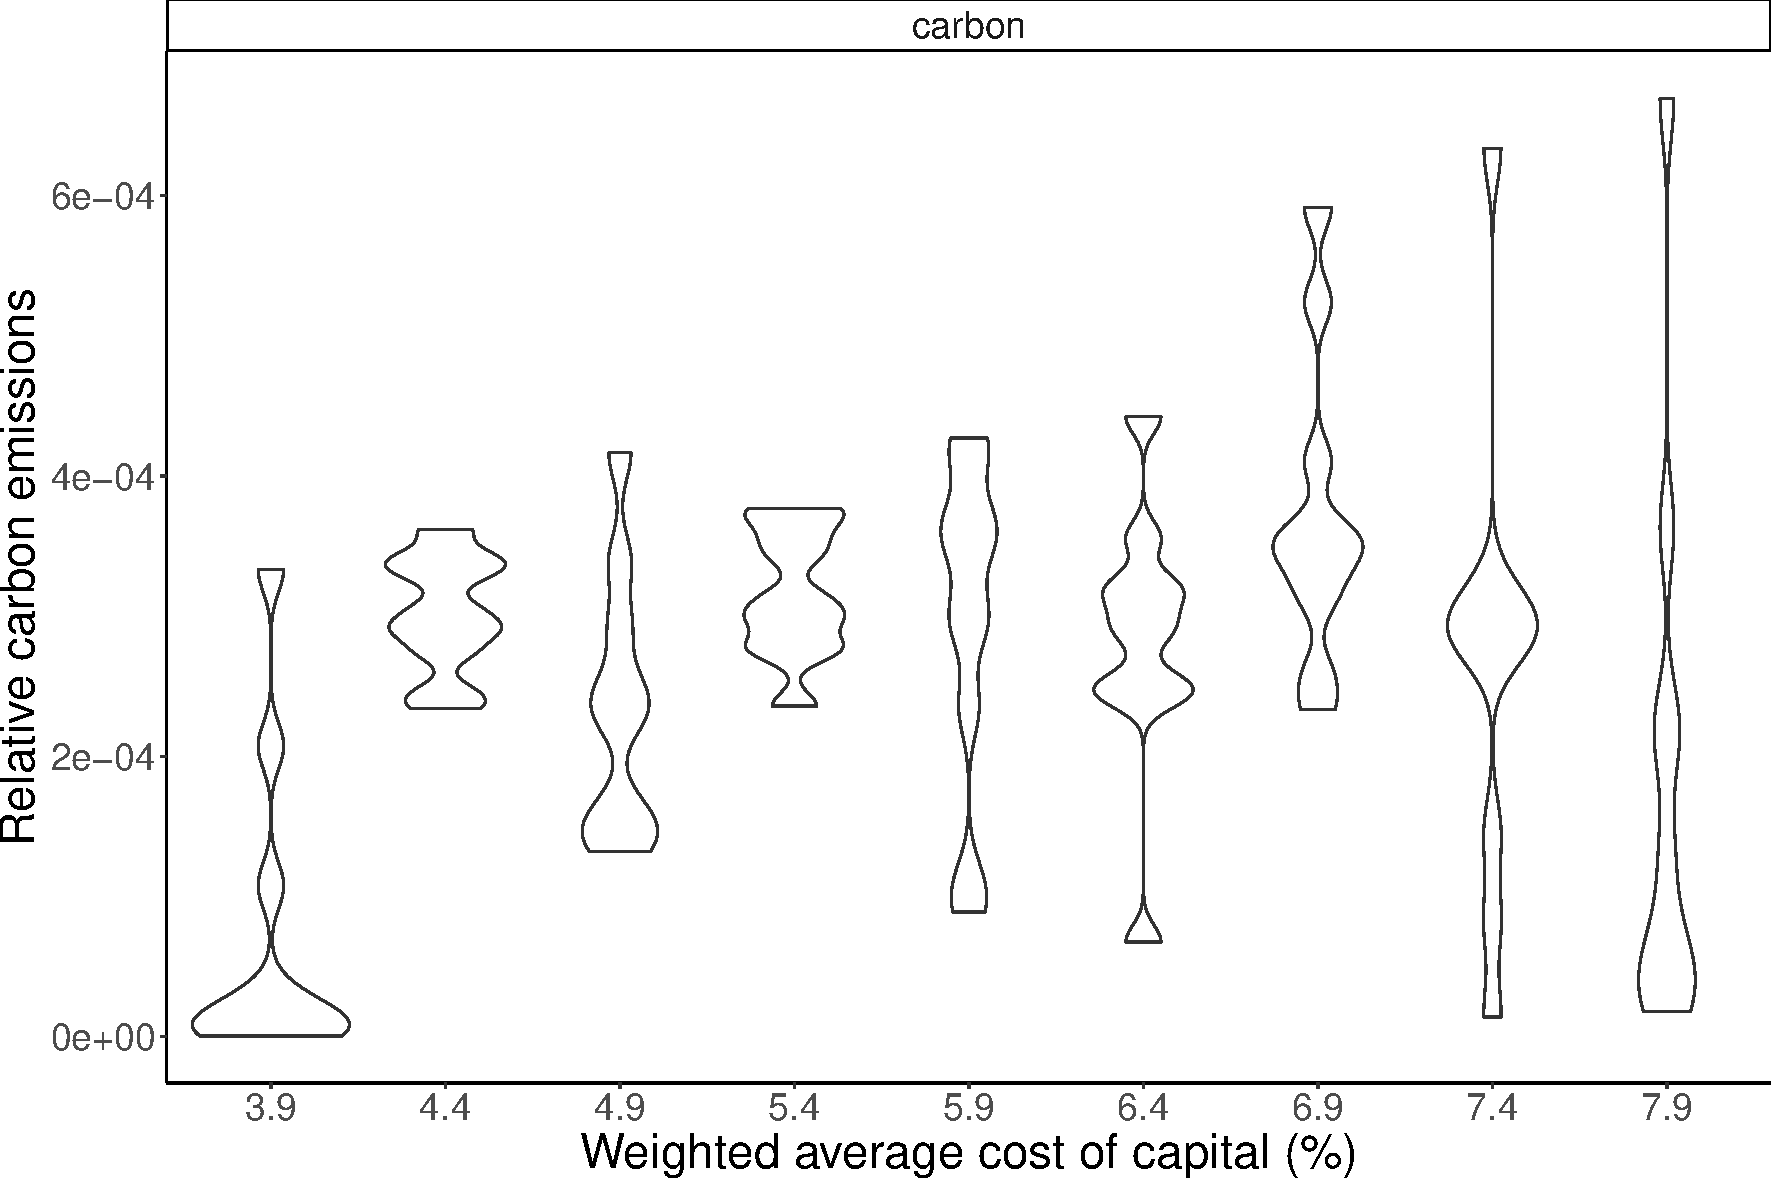
\includegraphics[width=0.9\linewidth]{Chapter4/figures/sensitvity_analysis/wacc_carbon_sensitivity_analysis.pdf}
	\caption{Sensitivity analysis where weighted average cost of capital (WACC) was varied. Results compare relative carbon emissions in 2035.}
	\label{elecsim:fig:wacc_carbon_sensitivity}
\end{figure}

Figure \ref{elecsim:fig:downpayment_sensitivity} displays the sensitivity analysis results for different levels of down payment required for all investments. We varied the down payment required between the values of 10\% and 40\%.

As down payment required increases, so does nuclear and onshore, whilst solar decreases. CCGT also shows an increase with down payment required. The increase in down payment may help nuclear, due to the high costs of \acrshort{wacc}. With a higher down payment, the total costs of the project will fall when compared to other, cheaper, generators. It is likely that nuclear displaces solar in this case. CCGT increases up until a 35\% down payment required. This may be due to the increased use of onshore wind, where CCGT and coal is required to fill for times of low wind speeds.

 

\begin{figure}
	\centering
	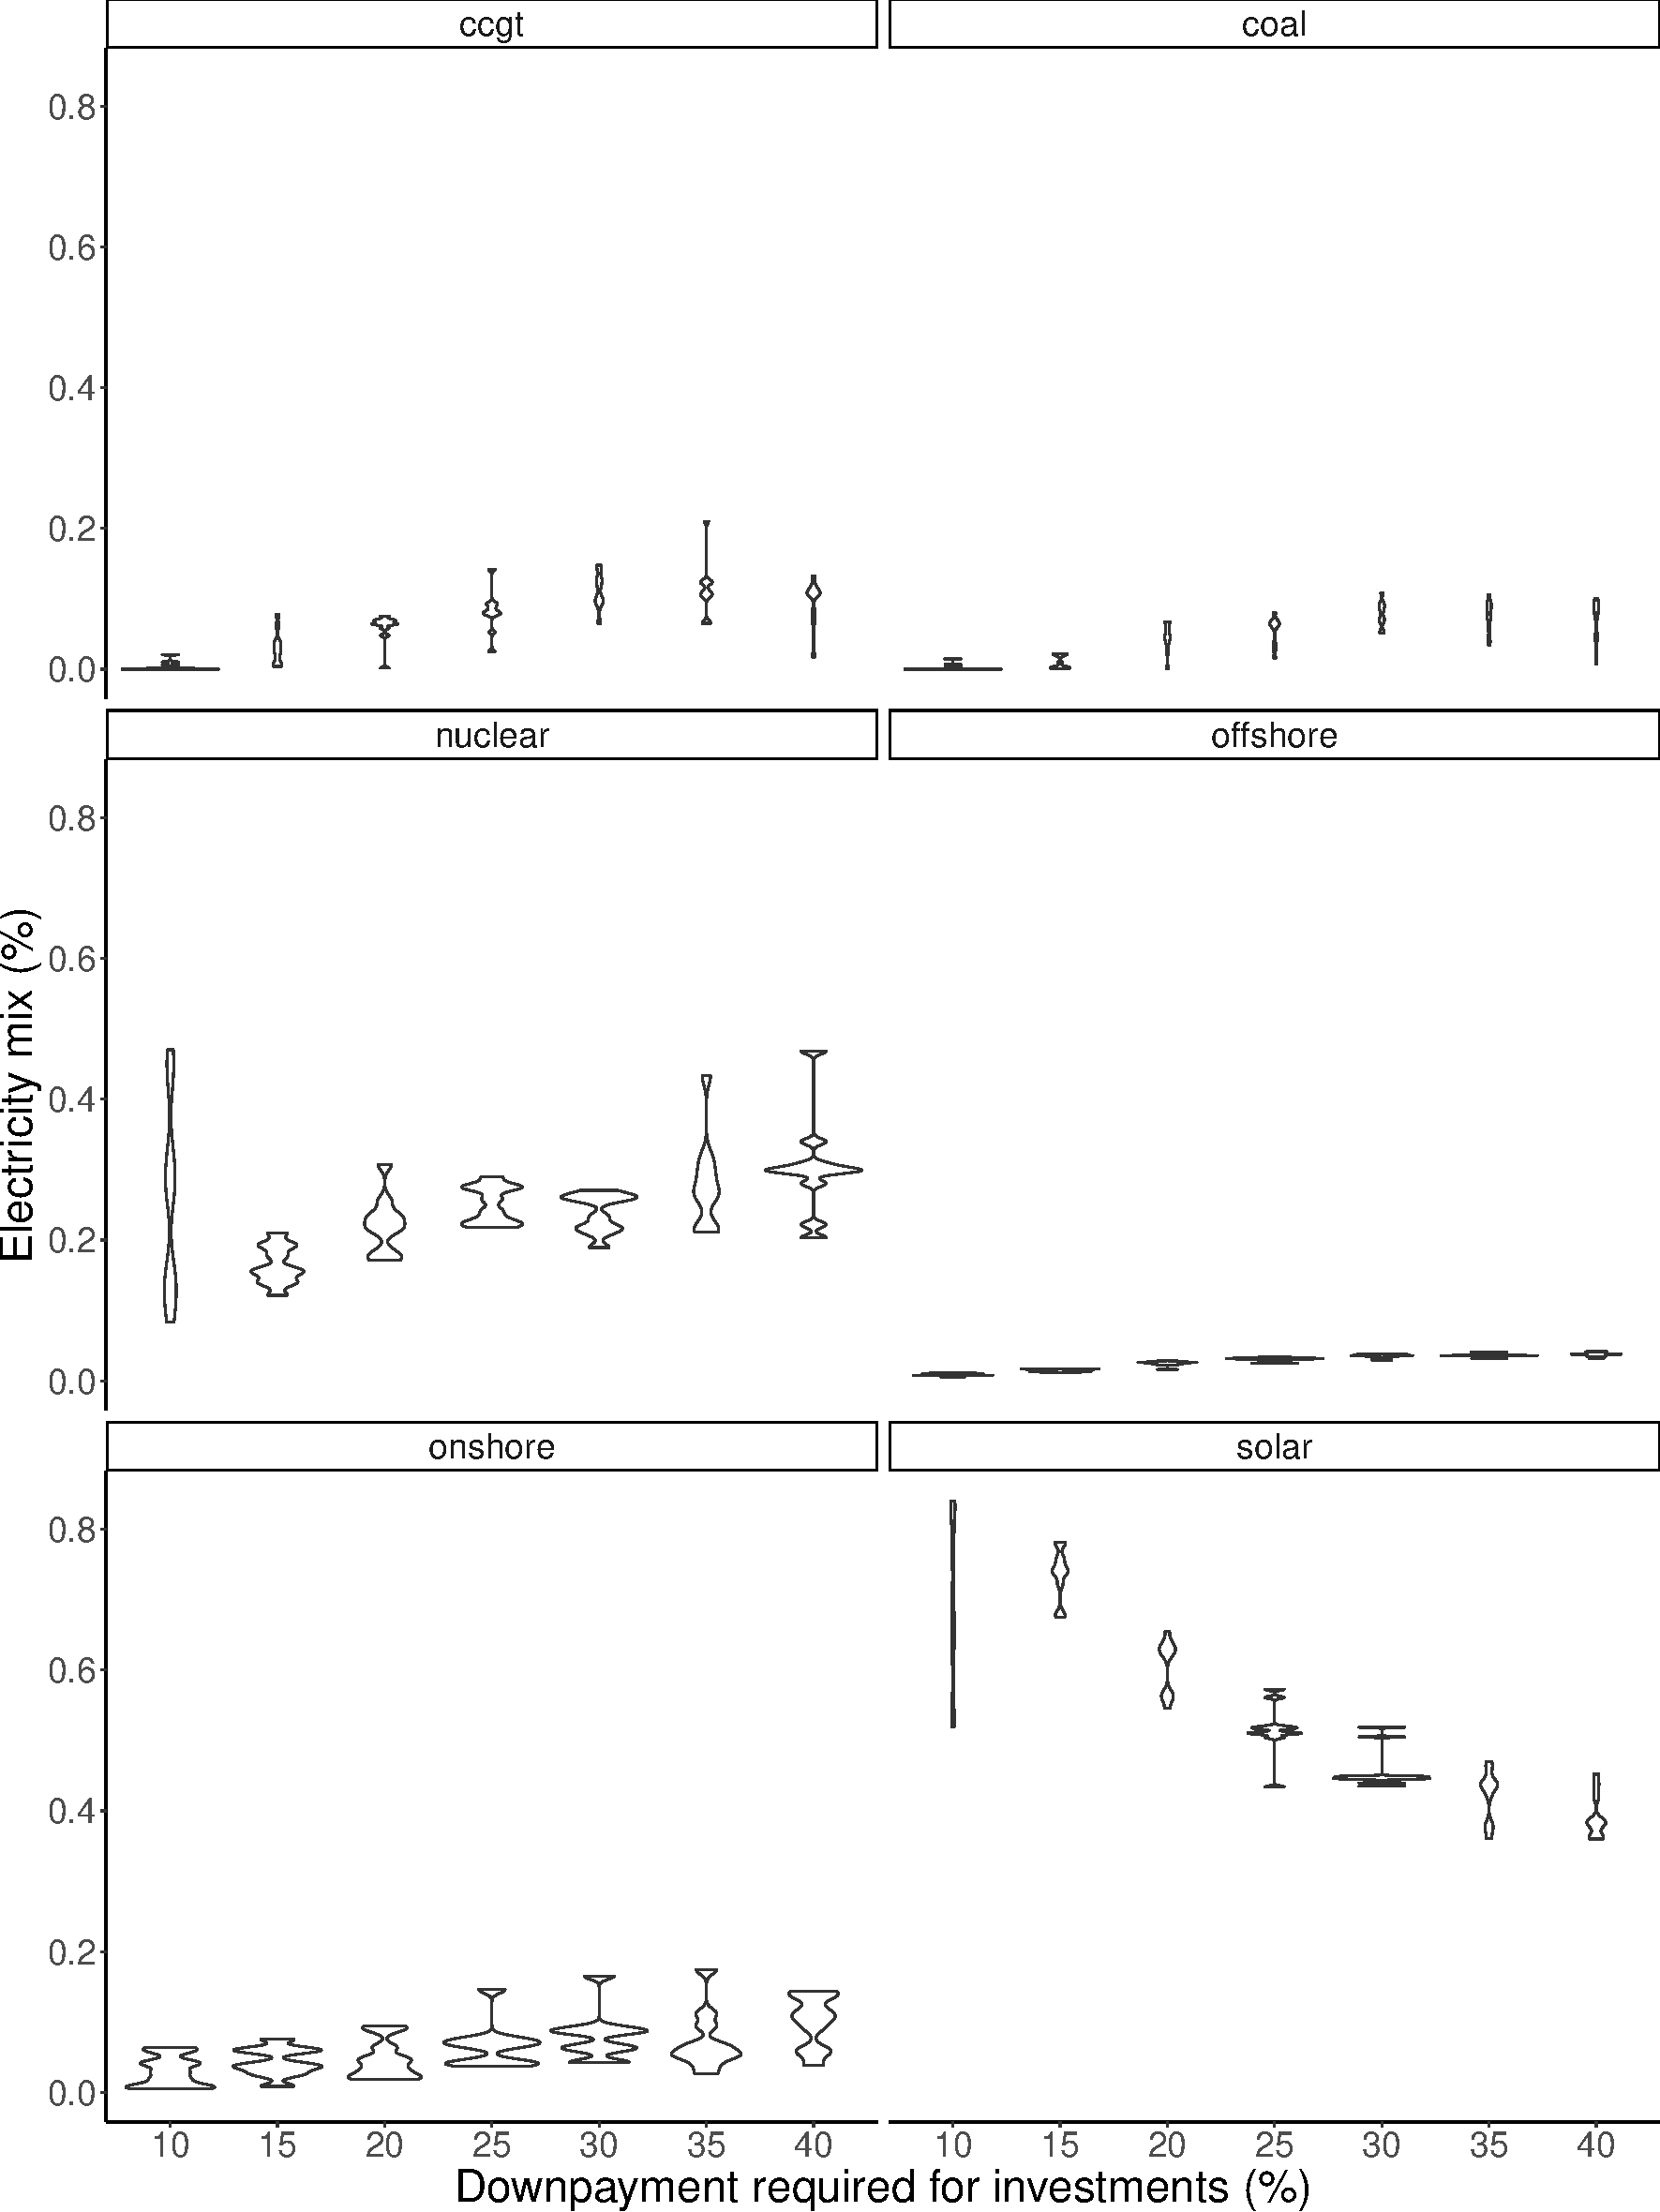
\includegraphics[width=0.9\linewidth]{Chapter4/figures/sensitvity_analysis/downpayment_sensitivity_analysis.pdf}
	\caption{Sensitivity analysis where percentage of down payment was varied. Results compare electricity mix in 2035.}
	\label{elecsim:fig:downpayment_sensitivity}
\end{figure}

Figure \ref{elecsim:fig:downpayment_carbon_sensitivity} displays the relative carbon emissions versus down payment required for investors. As down payment increases, so does relative carbon emissions. This is down to the increasing role that CCGT and coal play in the electricity mix, and decreasing solar capacity. 

A down-payment of 10\% seems to have the lowest carbon emissions. This is due to the high investment in solar, and low investment in CCGT and coal. 

\begin{figure}
	\centering
	\includegraphics[width=0.9\linewidth]{Chapter4/figures/sensitvity_analysis/downpayment_carbon_sensitivity_analysis.pdf}
	\caption{Sensitivity analysis where percentage of down payment was varied. Results compare relative carbon emissions in 2035.}
	\label{elecsim:fig:downpayment_carbon_sensitivity}
\end{figure}


\section{Limitations}

% Requirement of exogeneous price prediction curve
% Inability to validate on a long-term basis
% Lack of detailed supply curves (such as maximum wind and solar irradiance)
% Comparing to other models may not be correct as all models are wrong
% Future may change dramatically
% Lack of contracts for difference modelling and other subsidies (apart from nuclear)



\clearpage
\section{Conclusions}


%%%%%%%%%%%%%%%%%%%%%%%%%%%%%%%%%%%%%%%%%%%%%%%%
%%%%%%%%%%%%%%%%%%%%%%%%      Paper 1    %%%%%%%%%%%%%%%%
%%%%%%%%%%%%%%%%%%%%%%%%%%%%%%%%%%%%%%%%%%%%%%%%

Liberalised electricity markets with many heterogeneous players are suited to be modelled with ABMs. ABMs incorporate imperfect information as well as heterogeneous actors. ElecSim models imperfect information through forecasting of electricity demand and future fuel and electricity prices. This leads to agents taking risk on their investments, and model market conditions more realistically.

%We demonstrated that increasing carbon tax can lead to an increase in investment of low-carbon technologies. We showed that early decisions have a long-term impact on the energy mix. 

%Our future work includes comparing agent-learning techniques, using multi-agent reinforcement learning algorithms to allow agents to learn in a non-static environment. We propose the integration of a higher temporal and spatial resolution to model changes in daily demand, as well as capacity factors by region, and transmission effects. This will allow us to model that demand is met at all times and not just on average. 
%\begin{itemize}
%	\item Requirement for agent based models based on imperfect information, liberalised energy markets
%	\item Requirement for low barriers to entry open source model.
%	\item Discuss results
%	\item Future work:
%	\begin{itemize}
%		\item Embedding multi-agent intelligence such as Genetic Algorithms,  Q-learning and dynamic reinforcement learning
%		\item Raise spatial and temporal resolution.
%	\end{itemize}
%\end{itemize}



%%%%%%%%%%%%%%%%%%%%%%%%%%%%%%%%%%%%%%%%%%%%%%%%
%%%%%%%%%%%%%%%%%%%%%%%%      Poster    %%%%%%%%%%%%%%%%
%%%%%%%%%%%%%%%%%%%%%%%%%%%%%%%%%%%%%%%%%%%%%%%%





%%%%%%%%%%%%%%%%%%%%%%%%%%%%%%%%%%%%%%%%%%%%%%%%
%%%%%%%%%%%%%%%%%%%%%%%%      Paper 2    %%%%%%%%%%%%%%%%
%%%%%%%%%%%%%%%%%%%%%%%%%%%%%%%%%%%%%%%%%%%%%%%%




In this Chapter we have demonstrated that it is possible to use \acrshort{abm} to simulate liberalised electricity markets. Through validation, we are able to show that our model, ElecSim, is able to accurately mimic the observed, real-life scenario in the UK between 2013 and 2018. This provides confidence in the underlying dynamics of ElecSim, especially as we are able to model the fundamental transition between coal and natural gas observed between 2013 and 2018 in the UK.

In addition to this, we were able to compare our long-term scenario to that of the UK Government, Department for Business, Energy \& Industrial strategy. We show that we are able to mimic their reference scenario, however, demonstrate a more realistic increase in nuclear power. The parameters that were gained from optimisation show that the BEIS scenario is realistic, however a high nuclear subsidy may be required.

To improve the accuracy of our model, we used eight representative days of solar irradiance, offshore and onshore wind speed and demand to approximate an entire year. The particular days were chosen using a $k$-means clustering technique, and selecting the medoids. This enabled us to accurately model the daily fluctuations of demand and renewable energy resources. 

%We used a genetic algorithm to find the parameters that most closely matched the scenarios that we compared. The parameters found were realistic, providing confidence in the underlying dynamics of ElecSim.

%In future work we would like to evaluate further scenarios to provide advice to stakeholders, integrate multi-agent reinforcement learning techniques to better model agents in both investment and bidding strategies as well as model different countries. Further work could be to make predicted price duration curves endogenous to the model, however, this could require scenario analysis by each of the GenCos each time they wanted to make an investment.

In addition to this, a method of dealing with the non-validatable nature of electricity markets, as per the definition of Hodges \textit{et al.} is to vary input parameters over many simulations and look for general trends \cite{Hodges}. This could be achieved using ElecSim through the analysis of a reference case, and a limited set of scenarios which include the most important uncertainties in the model structure, parameters, and data, i.e. alternative scenarios which have both high plausibility and major impacts on the outcomes.

Additionally, we showed a number of scenarios, and shows that total demand has an effect on electricity mix. An increasing demand, year-on-year, can lead to an increase in solar to accommodate for this demand. However, if demand reduces, there is a higher investment in nuclear, which contributes to the electricity mix by 2034.

We ran a sensitivity analysis of \acrfull{wacc} and down payment required. We showed that these two variables have a large effect on total electricity mix by the year 2035, which in turn effects the total carbon emissions. We therefore show that the input assumptions have an effect on the simulation, which must be considered when analysing model outputs.


















